\documentclass[master=cws,masteroption=gs,english]{kulemt/kulemt}
\setup{title={Secure and protected data aggregation in the decentralized web},
  author={Jesse Geens},
  promotor={Prof. dr. ir. Wouter Joosen \and Dr. Bert Lagaisse \and Prof. dr. Vincent Naessens},
  assessor={Prof. dr. Bart Jacobs \and Dr. Emad Heydari Beni},
  assistant={Dr. Emad Heydari Beni \and Ir. Kristof Jannes}}
% De volgende \setup mag verwijderd worden als geen fiche gewenst is.
\setup{filingcard,
  translatedtitle={Veilige en beschermde gegevensaggregatie in het gedecentraliseerde web},
  udc=621.3,
  shortabstract={\begin{otherlanguage}{dutch}
{\small Solid is een W3C specificatie die tracht het web te decentraliseren met behulp van datakluizen. Datakluizen zijn gedecentraliseerde opslagplaatsen waar gegevens voor verschillende toepassingen worden bijgehouden. Een uitdaging hierbij is veilige en beschermde gegevensaggregatie over verschillende datakluizen heen. Dergelijke aggregaties brengen privacyrisico's met zich mee, net als schaalbaarheidsproblemen. Deze thesis introduceert een middleware die tracht deze problemen gedeeltelijk (op het niveau van de server) op te lossen, dankzij het introduceren van privacy filters en een nieuw mechanisme voor toegangstokens dat gedecentraliseerde tokenafvaardiging ondersteunt.
Privacy filters staan toe om meer granulariteit te bereiken in de privacy van gedeelde bronnen. De middleware selecteer hierbij automatisch transformaties die uitgevoerd worden wanneer een bron verzocht wordt, op basis van een aantal contextuele parameters. Om vervolgens een tokenmechanisme te bekomen dat gedecentraliseerde tokenafvaardiging ondersteunt onderzoekt deze thesis het gebruik van macaroons binnen Solid. Macaroons ondersteunen niet alleen gedecentraliseerde tokenafvaardiging, maar zijn ook effici{\"e}nter om te genereren en verifi{\"e}ren. Bovendien laten ze attesten van derde partijen toe, wat een nuttige eigenschap is voor datakluizen die gedeeld worden door een groep gebruikers.
De middleware die deze thesis voorstelt werd ge{\"e}valueerd op grond van drie gebruiksscenario's. Voor privacy filters hebben experimenten aangetoond dat de overhead van de middleware toelaatbaar is voor kleinere bronnen met een overhead van ongeveer 50\%. Echter, grotere bronnen (rond de 3MB) hebben een overhead die een vijfvoud wordt van de oorspronkelijke duur van het verzoek. 
Prestatietests die werden uitgevoerd op het genereren en verifi{\"e}ren van macaroons hebben aangetoond dat de doorvoer hiervan bij macaroons respectievelijk zeven en elf maal groter is dan het DPoP (ES256) systeem. Ten slotte zijn er ook theoretische winsten voor gedecentraliseerde tokenafvaardiging.}
\end{otherlanguage}
\\}}
% Verwijder de "%" op de volgende lijn als je de kaft wil afdrukken
%\setup{coverpageonly}
% Verwijder de "%" op de volgende lijn als je enkel de eerste pagina's wil
% afdrukken en de rest bv. via Word aanmaken.
%\setup{frontpagesonly}

% Kies de fonts voor de gewone tekst, bv. Latin Modern
\setup{font=lm}

%% TODO come up with name and insert it here
\newcommand{\mwprivacy}{PePSA}
\newcommand{\middleware}{MASS}

% PassOptionsToPackage fixes line breaks in URLs
\PassOptionsToPackage{hyphens}{url}\usepackage[pdfusetitle,colorlinks,plainpages=false]{hyperref}
\hypersetup{%
  citecolor=blue!70,
  linkcolor=black,
}

\usepackage{float}

% for formal definitions
\usepackage{framed}

% Fix "no room for new write" error
\usepackage{morewrites}

% Fancy quote in preface
\makeatletter
%\renewcommand{\@chapapp}{}% Not necessary...
\newenvironment{fancyquote}[2][2em]
  {\setlength{\@tempdima}{#1}%
   \def\fancyquote@author{#2}%
   \parshape 1 \@tempdima \dimexpr\textwidth-2\@tempdima\relax%
   \itshape}
  {\par\normalfont\hfill--\ \fancyquote@author\hspace*{\@tempdima}\par\bigskip}
\makeatother

% environment derived from framed.sty: see leftbar environment definition
%\newenvironment{formal}{%
%  \def\FrameCommand{%
%    \definecolor{formalshade}{rgb}{0.95,0.95,1}
%    \definecolor{darkblue}{rgb}{0.0, 0.0, 0.55}
%    \hspace{1pt}%
%    {\color{darkblue}\vrule width 2pt}%
%    {\color{formalshade}\vrule width 4pt}%
%    \colorbox{formalshade}%
%  }%
%  \MakeFramed{\advance\hsize-\width\FrameRestore}%
%  \noindent\hspace{-4.55pt}% disable indenting first paragraph
%  \begin{adjustwidth}{}{7pt}%
%  \vspace{2pt}\vspace{2pt}%
%}
%{%
%  \vspace{2pt}\end{adjustwidth}\endMakeFramed%
%}

\newcounter{futurework}
\newenvironment{futurework}[1][]{\refstepcounter{futurework}\par\medskip
   \noindent \textbf{FW~\thefuturework #1} \rmfamily}{\medskip}

% multi-column enumerate in evaluation
\usepackage{multicol}

% cite (author, year) style
\usepackage{natbib}
%\bibliographystyle{abbrvnat}
\bibliographystyle{unsrtnat}
\setcitestyle{authoryear,open={(},close={)}}
\newcommand{\citepjournal}[1]{(\citetalias{#1}, \citeyear{#1})}
\newcommand{\citetjournal}[1]{\citetalias{#1} (\citeyear{#1})}

% Set todos in text
\usepackage{todonotes}

% % For SAPlugin diagrams
\usepackage{rotating}
\usepackage{pdflscape}
\usepackage{amsmath}
\usepackage{minitoc}
\usepackage[sort]{cleveref}
\usepackage{xparse}
\usepackage{expl3}
\usepackage{enumitem}
\usepackage{minitoc}
\usepackage{advdate}
\usepackage{pdftexcmds,xparse}
\usepackage{totcount}
\usepackage{lcg}
\usepackage{fontawesome}
\usepackage{tikz,pgfplots}
\usetikzlibrary{positioning,fit}
\usetikzlibrary{arrows}

% item labels
\makeatletter
\def\vpeitemlabel#1#2{\begingroup
	#2%
	\def\@currentlabel{#2}%
	\phantomsection\label{#1}\endgroup
}
\makeatother

\newcommand*\vpejustify{%
	\fontdimen2\font=0.4em%
	\fontdimen3\font=0.8em%
	\fontdimen4\font=0.1em%
	\fontdimen7\font=1.0em%
	\hyphenchar\font=`\-\relax%
}
\newcommand{\vpett}[1]{\vpejustify{\texttt{#1}}}
% vpe operation
\newcommand{\vpeoperation}[1]{#1}

% vpe data type
\newcommand{\vpedatatype}[2]{\vpeitemlabel{#1}{\textbf{\textsf{#2}}}}

% vpe exception
\newcommand{\vpeexception}[2]{\vpeitemlabel{#1}{\textsl{#2}}}

\newcommand{\iconcomponent}{%
	\begin{tikzpicture}[scale=0.3,thin,baseline=-0.05ex]
	\draw (0,0) rectangle (0.4, 0.6);
	\draw [fill=white] (-0.1,0.40) rectangle +(0.25, 0.1);
	\draw [fill=white] (-0.1,0.22) rectangle +(0.25, 0.1);	
	\end{tikzpicture}%
}
\newcommand{\iconprovided}{%
	\begin{tikzpicture}[scale=0.25,thin,baseline=-0.25ex]
	\draw (0.60,0.25) circle [radius=0.25];
	\draw (0, 0.25) -- (0.35, 0.25);
	\end{tikzpicture}%
}
\newcommand{\iconrequired}{%
	\begin{tikzpicture}[scale=0.25,thin,baseline=-0.25ex]
	\draw (0.60,0) arc (270:90:0.25);
	\draw (0, 0.25) -- (0.35, 0.25);
	\end{tikzpicture}%
}
\newcommand{\iconinher}{%
	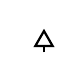
\begin{tikzpicture}[scale=0.3,thick,baseline=-0.5ex]
	\node (0,0) {};
	\draw[-open triangle 60] (.3,-.4) -- (.3, .6);
	\node (.9,0) {};
	\end{tikzpicture}%
}

%%%%%%%
% Custom code listings
\usepackage{listings}
\usepackage{color}
\usepackage{chngcntr}

% Enumerations with letters instead of numbers
\usepackage{enumitem}

% For optional reading section
\usepackage[most]{tcolorbox}
\definecolor{myblue}{RGB}{0, 151, 238}
\definecolor{accent}{RGB}{87, 255, 220}

% Subfigures
\usepackage{subcaption}

% Acronyms
\usepackage[acronym,smallcaps]{glossaries}
\glstoctrue
\loadglsentries{acronyms}
\makeglossaries
%\glsdisablehyper

% Default fixed font does not support bold face
\DeclareFixedFont{\ttb}{T1}{txtt}{bx}{n}{12} % for bold
\DeclareFixedFont{\ttm}{T1}{txtt}{m}{n}{12}  % for normal

% Support for source code listings
\usemintedstyle{autumn}

\newenvironment{code}{\captionsetup{type=listing}}{}
\renewcommand{\lstlistlistingname}{List of code fragments}
%\SetupFloatingEnvironment{listing}{name=Listing}




%%%%%%%%%
% Fix quotes, see https://tex.stackexchange.com/questions/356898/quote-with-author-reference-at-the-end
\let\oldquote\quote
\let\endoldquote\endquote
\renewenvironment{quote}[2][]
  {\if\relax\detokenize{#1}\relax
     \def\quoteauthor{#2}%
   \else
     \def\quoteauthor{#2~---~#1}%
   \fi
   \oldquote}
  {\par\nobreak\smallskip\hfill(\quoteauthor)%
   \endoldquote\addvspace{\bigskipamount}}

% No horizontal table overflows
\usepackage{tabulary}

% For drawing access tree structure with tikz
\usepackage{tikz-qtree}

%set default line width to 0.75pt     
\tikzset{every picture/.style={line width=0.75pt}} 

% Draw boxplots
\usepackage{pgfplots}
\pgfplotsset{compat=1.8}
\usepgfplotslibrary{statistics}

% Turn images 90 degrees
\usepackage{rotating}

% Remove capitalization
\addto\captionsenglish{%
  \renewcommand\listfigurename{List of figures}}
  
\addto\captionsenglish{%
  \renewcommand\listtablename{List of tables}}
  
%\includeonly{chap-n}
\begin{document}

% Include bibliography aliases for citing journals
\defcitealias{solid-sweden}{De Tijd}
\defcitealias{solid-flanders}{De Tijd}
\defcitealias{inrupt-seriesa}{TechCrunch}
\defcitealias{mckinsey-privacy}{McKinsey}


% Make listing numbers follow chapters
\counterwithin{lstlisting}{chapter}

\begin{preface}
\begin{fancyquote}{\textit{Sir Tim Berners-Lee}}
``I found myself answering the same questions asked frequently of me by different people. It would be so much easier if everyone could just read my database.''
\end{fancyquote}

\noindent Solid is an amazing technology that has the potential to change the web as we know it. The last year, I have witnessed amazing progress being made in this domain, and I am truly honored that I had the opportunity to be a part of it. It has been quite the roller coaster, combining my dissertation research with a semester spent abroad on an Erasmus exchange, but it was well worth the effort. There are an endless amount of people I want to thank for supporting me through this period, especially my friends and family.\\

\noindent First and foremost, my most sincere gratitude goes to my girlfriend Elise, who had to endure endless streams of complaints when I was stuck somewhere, and screams of joy when I made some progress. Without her support, this text would not be the same.\\

\noindent Secondly, I owe an immense amount of gratitude to my supervisors and assistant-supervisors. 
In particular, I want to thank Bert Lagaisse for allowing me to combine my dissertation while studying in Hungary, which was not a trivial task. Your feedback and guidance taught me a lot and greatly improved the quality of my work. I also want to thank Emad and Kristof for the great advice and encouragement every week. Your advice has inspired me many times and your kind words have always encouraged me. Finally, I also want to explicitly thank prof. Vincent Naessens, prof. Wouter Joosen and Dimitri Van Landuyt for their valuable feedback and suggestions.\\

\noindent Thirdly, I want to thank my family for supporting me not only through this dissertation, but throughout my whole study career. I owe a large part of my successes to their support. I especially want to thank my father and grandfather for inspiring me to study a technical domain, and for teaching me to always think critically.\\

\noindent Lastly, I want to thank my father and my friends Benjamin, Aram and Tobias for proofreading and improving this text. 

\end{preface}

\tableofcontents*

\begin{abstract}
  In recent years, the internet has become evermore centralized \citep{internet-report}. This has many negative side effects, such as decreased competition and a lack of access to personal data \citep{big-tech-innovation, platform-monopolies}. Solid \citep{solid} is a new draft W3C specification that aims to combat this by introducing pods. Pods are decentralized datastores where user data is kept for many different applications. In this manner, the user retains control over his personal data, and the same data can be used across different services.
  
  These pods provide a number of possibilities, but also come with technological challenges. One such challenge is secure and protected data aggregation across different pods. Such data aggregations impose privacy risks, as well as scalability issues. This dissertation presents a server-level middleware that aims to partially resolve these issues by presenting two novel technologies: privacy filters, and a new token mechanism that supports decentralized delegation.
  
  Privacy filters is a technology that enables more granularity in the privacy of shared resources. When a request is made, the middleware selects a number of transformations to perform on the requested resource, based on the user's settings and contextual parameters such as the requesting application and the resource's data type. To subsequently attain a token mechanism that supports decentralized delegation, this dissertation investigates the use of macaroons as a token mechanism in Solid. Macaroons not only provide decentralized token delegation, but are also much more efficient to generate and verify. Moreover, they allow third-party attestations, which is a useful property for realizing pods belonging to a group of agents.
  
  The middleware presented in this dissertation has been evaluated on the basis of three use cases. For privacy filters, a number of performance experiments have demonstrated that the overhead of the middleware is tolerable for smaller resources. Rewriting resources of around 300KB using three transformations causes an overhead of around 50\% in the request duration. However, larger resources (around 3MB) have overheads that become a five-fold of the original request duration. As such, a more efficient method for resource rewriting may be necessary here, although this issue can be lessened by making use of caching and precomputation. Performance experiments on the generation and verification of macaroons have illustrated that macaroons offer large performance benefits. The throughput of generating and verifying macaroons is seven and eleven times higher respectively, compared to \acrshort{DPoP} using the ES256 algorithm. Finally, there are also theoretical gains for decentralized delegation in a reduced number of needed interactions for realizing token delegation.
\end{abstract}

\begin{abstract*}
  De afgelopen jaren is het internet steeds meer gecentraliseerd geworden \citep{internet-report}. Dit heeft vele negatieve gevolgen, waaronder gedaalde concurrentie en een gebrek aan toegang tot persoonlijke gegevens \citep{big-tech-innovation, platform-monopolies}. Solid \citep{solid} is een nieuwe voorlopige W3C specificatie die dit probleem tracht op te lossen door het introduceren van datakluizen. Datakluizen zijn gedecentraliseerde opslagplaatsen voor data waar gegevens voor verschillende toepassingen worden bijgehouden. Op deze manier bewaart de gebruiker controle over zijn persoonlijke gegevens, en kan dezelfde data door verschillende diensten gebruikt worden.
  
  Deze datakluizen brengen een hoop mogelijkheden met zich mee, maar evenzeer technologische uitdagingen. Een van zo'n uitdagingen is de veilige en beschermde gegevensaggregatie over verschillende datakluizen heen. Dergelijke aggregaties brengen privacyrisico's met zich mee, net als schaalbaarheidsproblemen. Deze thesis introduceert een middleware op het niveau van de server, die tracht deze problemen gedeeltelijk op te lossen dankzij het introduceren van twee nieuwe technologie{\"e}n. Deze technologie{\"e}n zijn privacy filters en een nieuw mechanisme voor toegangstokens dat gedecentraliseerde tokenafvaardiging ondersteunt.

  Privacy filters is een technologie die toelaat om meer granulariteit te bereiken in de privacy van gedeelde bronnen. Wanneer een verzoek gemaakt wordt selecteert de middleware automatisch een aantal transformaties die uitgevoerd worden op de verzochte bron. Dit gebeurt gebaseerd op een aantal contextuele parameters, zoals welke toepassing het verzoek verzonden heeft of wat het data type is van de verzochte bron. Om een tokenmechanisme te bekomen dat gedecentraliseerde tokenafvaardiging ondersteunt onderzoekt deze thesis het gebruik van macaroons als nieuw tokenmechanisme binnen Solid. Macaroons ondersteunen niet alleen gedecentraliseerde tokenafvaardiging, maar zijn ook effici{\"e}nter om te genereren en verifi{\"e}n. Bovendien laten ze getuigenissen van derde partijen toe (\textit{third-party attestations}), wat een nuttige eigenschap is om datakluizen te bekomen die gedeeld worden door een groep gebruikers.
  
  De middleware die deze thesis voorstelt werd ge{\"e}valueerd op grond van drie gebruiksscenario's. Voor privacy filters hebben een aantal prestatie-experimenten aangetoond dat de overhead van de middleware toelaatbaar is voor kleinere bronnen. Het herschrijven van bronnen tot 300KB gebruikmakende van drie transformaties leidt tot een overhead van ongeveer 50\%. Echter, grotere bronnen (rond de 3MB) hebben een overhead die een vijfvoud wordt van de oorspronkelijke duur van het verzoek. Zodanig kan een effici{\"e}nter mechanisme voor het herschrijven van bronnen hier bruikbaar zijn, hoewel dit probleem kan verminderd worden door gebruik te maken van caches, of met behulp van voorberekeningen. Prestatie-experimenten die werden uitgevoerd op het genereren en verifi{\"e}ren van macaroons hebben aangetoond dat hier sterke prestatievoordelen aan vasthangen. De doorvoer voor het genereren en verifi{\"e}n van macaroons is respectievelijk zeven en elf maal groter dan het \acrshort{DPoP} systeem wanneer dit gebruik maakt van het ES256 algoritme. Ten slotte zijn er ook theoretische winsten voor gedecentraliseerde tokenafvaardiging, gezien dit mechanisme een verminderd aantal interacties nodig heeft voor het afvaardigen van een toegangstoken in vergelijking met een gecentraliseerd mechanisme zoals \acrshort{DPoP}.
\end{abstract*}

% Een lijst van figuren en tabellen is optioneel
%\listoffigures
%\listoftables
% Bij een beperkt aantal figuren en tabellen gebruik je liever het volgende:
%\renewcommand\listoflistingscaption{List of Source Codes}
\makeatletter\@openrightfalse
\listoffiguresandtables
%\lstlistoflistings
%\phantomsection
%\addcontentsline{toc}{chapter}{\lstlistlistingname}{
\lstlistoflistings%}

\addcontentsline{toc}{chapter}{List of code fragments and repositories}{
{\let\clearpage\relax \chapter*{List of repositories}}
\begin{tabularx}{\textwidth}{@{}p{37mm}X@{}}
    \texttt{pepsa-component}   & \url{https://github.com/jessegeens/pepsa-component} \\
    \texttt{groupvault-demo}   & \url{https://github.com/jessegeens/groupvault-demo} \\
    \texttt{data-generator}   & \url{https://github.com/jessegeens/data-generator} \\
    \texttt{thesis-experiments}   & \url{https://github.com/jessegeens/thesis-experiments} \\
    %All code (KU Leuven only)   & \url{https://github.com/jessegeens/pepsa-component} \\
  \end{tabularx}
}

 

\printglossary[type=\acronymtype,title={List of abbreviations}]
\@openrighttrue\makeatother



% De lijst van symbolen is eveneens optioneel.
% Deze lijst moet wel manueel aangemaakt worden, bv. als volgt:
%\chapter{List of Abbreviations}
%\section*{Abbreviations}
%\begin{flushleft}
%  \renewcommand{\arraystretch}{1.1}
%  \begin{tabularx}{\textwidth}{@{}p{20mm}X@{}}
%  \end{tabularx}
%\end{flushleft}
%\section*{Symbols}
%\begin{flushleft}
%  \renewcommand{\arraystretch}{1.1}
%  \begin{tabularx}{\textwidth}{@{}p{12mm}X@{}}
%    42    & ``The Answer to the Ultimate Question of Life, the Universe,
%            and Everything'' according to \cite{h2g2} \\
%    $c$   & Speed of light \\
%    $E$   & Energy \\
%    $m$   & Mass \\
%    $\pi$ & The number pi \\
%  \end{tabularx}
%\end{flushleft}

% Nu begint de eigenlijke tekst
\mainmatter

\chapter{Introduction}
\label{cha:intro}
%The first contains a general introduction to the work. The goals are
%defined and the modus operandi is explained.

\section{Problem Statement}

\section{Contributions}

\section{Thesis Outline}
\chapter{Background}
\label{cha:background}
This thesis investigates a middleware for de-identifying data exposed through the Solid protocol. Section \ref{sec:solid} introduces the basic concepts of Solid, while section \ref{sec:pets} introduces some necessary background knowledge on \gls{PETs}.

\section{Solid}
\label{sec:solid}

\subsection{Introduction}
\begin{quote}{Tim Berners-Lee}
    The Semantic Web is not a separate Web but an extension of the current one, in which information is given well-defined meaning, better enabling computers and people to work in cooperation.
\end{quote}

\noindent In 2001, Sir Tim Berners-Lee - the inventor of the world-wide web - published an article in \textit{Scientific American} entitled `The semantic Web' \citep{semantic-web}. It envisioned a future where the Web was not just a collection of pages with meaningless links to each other, but a smart Web, where objects have well-defined meanings.

Today, most resources accessible on the Web are meant for people to read, understand and process, but it is not adapted to automated processing by software agents. Computers can read information and format it correctly, but they lack a unified way to interpret the information: there is no way to process the \textit{semantics}. The Semantic Web tries to solve this problem by extending the current Web with new, compatible standards and protocols to attach computer-readable meaning to information available on the Web.

Currently, markup languages such as XML enable users to arbitrarily structure documents the way they want it (e.g. using a tag called \texttt{<book>} and a tag called \texttt{<isbn>}). They then write software that parses this by telling the software that \texttt{<book>} means "book" and \texttt{<isbn>} means "isbn". However, other users may use different terms (e.g. \texttt{<livre>}), making information not universally parsable. 

\noindent The Semantic Web introduces the \gls{RDF}, which encodes structure and information in sets of triples: a subject, a predicate and an object. These triples  then create a knowledge graph called an RDF graph, where predicates relate subjects to objects. The objects in one triple can then be the subjects in another one. The figure below illustrates an example, where Tokyo is the subject of a linked data triple, and two predicates relate it to its area and the country it resides in. The object, Japan, may then be the subject of other RDF graphs, relating it for example to its population.

\begin{figure}[H]
    \centering
    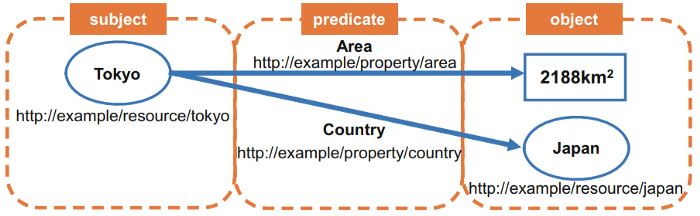
\includegraphics[width = 0.9\textwidth]{images/background/linked-data.png}
    \caption{\gls{RDF} representation of the city Tokyo, with predicates relating it to its area and its country. Source: \citet{generating-pva}}
    \label{fig:linked-data}
\end{figure}

\noindent Subjects, predicates and objects are all identified by a URI, making them universal, and allowing anyone to define new predicates\footnote{Unless they are literals, such as the area in the example}. Like this, webs of information are formed between related objects using definitions that can be found and understood by everyone.

This does not completely solve the problem, however. It is possible that multiple definitions exist for essentially the same object. To resolve this, the Semantic Web introduces a third component: ontologies. Ontologies are documents that formally define the relations among terms \citep{semantic-web}. A widely-used ontology is called \textit{foaf}\footnote{\url{ http://xmlns.com/foaf/spec/}} (friend-of-a-friend): it is used to describe relationships between people.

\gls{RDF}, however, is only something conceptual (a collection of subject, predicate and object). If we want to actually use it, we need to store \gls{RDF} in documents. This is possible in multiple ways, i.e., multiple representation formats exist. The most popular ones are Turtle \citep{turtle} and JSON-LD \citep{jsonld}. Turtle has the advantage that it allows you to define prefixes at the top of the file, which are aliases for the long URIs that you use to relate the subjects/predicates/objects. If you want to talk about the foaf ontology, you can define at the top of your file:

\texttt{@prefix foaf <http://xlmns.com/foaf/0.1/>}

\noindent You can then use \texttt{foaf} in the rest of your turtle file, instead of \texttt{<http://xlmns.com/\\foaf/0.1/>}. This makes it very human-readable compared to other formats. Additional existing formats are \gls{RDF}/XML and N-Triples, but they are less common.

\subsection{The Solid Protocol}
\begin{quote}{\href{https://solidproject.org}{solidproject.org}}
    Solid is a proposed set of conventions and tools for building \textit{decentralized applications} based on Linked Data principles.
\end{quote}
\noindent Solid \citep{solid} is a proposed W3C specification that wishes to decentralize the web by giving people control over their data. Solid aims to realize this by giving people an online datastore called a \textit{pod} (personal online datastore). Users can then login to applications using an authentication mechanism provided by Solid, and the application can in turn access data stored in the user's pod.

By storing all the data inside the user's pod instead of on the application server, the user retains complete control over his data. He can flexibly choose what data to share with what applications. Furthermore, storing the data in a pod reduces vendor lock-in: when the user wishes to switch from one service to another, he can simply give the new application access to the data he already possesses. 
In Solid, there are two types of resources: linked and non-linked data resources. Non-linked data resources are the usual kinds of data that we access on the web right now (binary, text, images, ...), while linked data follows the 
 \gls{RDF} specifications by using a content representation such as Turtle. These linked-data standards follow the principles of the Semantic Web.

\subsection{Authentication}
Authenticating a user is the act of verifying a user's claimed identity. Identities in solid (both for users and other agents) follow the WebID standard \citep{webid}: URIs act as universal identifiers. An example WebID is:

\begin{center}
   \texttt{https://jessegeens.solidcommunity.net/profile/card\#me}\\
\end{center}

\noindent These WebID URIs can identify several things: users, software agents, or other things (even if they do not exist on the web). The WebID URI references a WebID Profile Document. This document contains information about the agent who is the referent of the WebID URI. However, an important distinction must be made. When the \textit{\texttt{\#me}} is included in the URI (or more in general, the hashtag), this URI refers to an agent. When the hashtag is omitted, the URI refers to the document describing this agent.

While the WebID standard provides identities, it does not yet verify them. The actual authentication (or, verifying that the agent actually controls the WebID he claims to control) in Solid uses the WebID-OIDC protocol. This protocol draws inspiration from OAuth2 and from OpenID Connect. The below workflow, drawn from the WebID-OIDC repository, explains the basic mechanism of the protocol:

\todo{Also here, make sure this is not plagiarism, since it is copied from the repo}

\begin{quote}{\href{https://github.com/solid/webid-oidc-spec}{webid-oidc-spec repository}}

    1. \textbf{Initial Request}: Alice (unauthenticated) makes a request to bob.example, receives a \texttt{HTTP 401 Unauthorized} response, and is presented with a 'Sign In With...' screen.\\
    
    2. \textbf{Provider Selection}: She selects her WebID service provider by clicking on a logo, typing in a URI (for example, alice.solidtest.space), or entering her email.\\
    
    3. \textbf{Local Authentication}: Alice gets redirected towards her service provider's own Sign In page, thus requesting https://alice.solidtest.space/signin, and authenticates using her preferred method (password, WebID-TLS certificate, FIDO 2 / WebAuthn device, etc).\\
    
    4. \textbf{User Consent}: (Optional) She's presented with a user consent screen, along the lines of "Do you wish to sign in to bob.example?".\\
    
    5. \textbf{Authentication Response}: She then gets redirected back towards https://bob.example/resource1 (the resource she was originally trying to request). The server, bob.example, also receives a signed ID Token from alice.solidtest.space that was returned with the response in point 3, attesting that she has signed in.\\
    
    6. \textbf{Deriving a WebID URI}: bob.example (the server controlling the resource) validates the ID Token, and extracts Alice's WebID URI from inside it. She is now signed in to bob.example as user https://alice.solidtest.space/\#i.\\
    
    7. \textbf{WebID Provider Confirmation}: bob.example confirms that solidtest.space is indeed Alice's authorized OIDC provider (by matching the provider URI from the iss claim with Alice's WebID).

\end{quote}

\subsection{Authorization}
Authorization within the Solid project builds on the Web Access Control standard \citep{wac}. The WAC standard provides a method to define authorization conditions for resources in a Pod using an \gls{ACL}.\todo{Explain here what an access control list is?} Every resource is coupled with an \gls{ACL} resource - either directly, or by inheriting it from a parent container. These \gls{ACL} resources are using the ACL ontology, usually in a turtle file\footnote{Other \gls{RDF} representations are also allowed, but support for turtle files is mandatory}. Authorization conditions consist of three elements: access objects (the associated resource), access modes (\textit{read}, \textit{write}, \textit{append} or \textit{control}) and access subjects (the agents performing the request).

The access objects in an \gls{ACL} resource are the resources the \gls{ACL} resource refers to. This can be both a normal resource (LDP-RS or LDP-NR, see \ref{subsec:ldp}) as well as a container. It is not mandatory for resources to have an associated ACL resource, as these can be inherited. This mechanism ensures that there is no need to create duplicate ACL resources for similar resources, as well as ensuring proper protection for newly created resources. When a resource is accessed, the server will first look for a directly associated \gls{ACL} resource. When none is found, the server will walk up the container tree (starting from the current container the resource is located in, then the parents, up until the root container). Once an \gls{ACL} resource applying to one of the parent containers is found, this is applied to the requested resource.

Possible access modes, then, are either \textit{read}, \textit{write}, \textit{append} or \textit{control}. Reading and writing are the usual operations. Append is a subset of writing: data can be added to the resource, but not deleted. This is useful for, for example, logging applications, ensuring that logs cannot be removed. Since appending is a subset of writing, the writing authorization implies the appending authorization (no resource can allow writing but disallow appending). Finally, control means being able to modify the ACL of the resource. Being able to control a resource generally implies ownership of the resource.

Lastly, access subjects are those agents who request a certain operation on the resource. Generally, these can be divided into four categories. The first one is \textit{every agent}, i.e., the resource is publicly accessible. A second option is authenticated agents only (with no restrictions on who these agents are), which may be useful for auditing purposes. Thirdly, resource access can be restricted to agents with a specific WebID. Finally, this can also be extended to groups of agents (where the group has a single WebID). An example \gls{ACL} resource, taken from the Solid Community Server\footnote{See \url{https://github.com/solid/community-server}}, is presented below:
\lstinputlisting[style=turtle, title=.acl, caption=Access Control List Resource]{code/acl.ttl}

\subsection{Linked Data Platform and Containers}
\label{subsec:ldp}
Solid mainly relies on the \gls{LDP} protocol \citep{ldp} for resource management. The \gls{LDP} protocol uses HTTP for accessing and modifying resources on a server. LDP Resources, or LDPRs, are HTTP resources that conform to a number of conventions. There are multiple types of resources:
\begin{enumerate}
    \item \gls{RDF} Sources, also called LDP-RSs (LDP \gls{RDF} Source)
    \item Non-\gls{RDF} Sources, such as images or binary data, which are called LDP-NRs
    \item Containers, a concept for bundling related resources together. These are also called LDPCs (LDP Container). 
\end{enumerate}

\noindent To support the access and modification of these resources, \gls{LDP} servers must support a number of HTTP methods on the resources. The \texttt{GET} method is mandatory and returns the request resource, if certain conditions are met (e.g., does the agent have the correct authorizations to access the resource). The \texttt{POST} and \texttt{PUT} methods are optional, and allow agents to create new resources or modify existing ones. Similarly, the \texttt{DELETE} method is optional and allows agents to delete resources. The \texttt{HEAD} and \texttt{OPTIONS} methods are mandatory to be implemented by servers and are similar to the methods defined in the HTTP/1.1 protocol. Below is an example of a request for a basic container and the accompanying reply \citep[from][]{ldp-primer}:

\begin{verbatim}
GET /alice/ HTTP/1.1
Host: example.org
Accept: text/turtle
HTTP/1.1 200 OK 
Content-Type: text/turtle; charset=UTF-8
Link: <http://www.w3.org/ns/ldp#BasicContainer>; rel="type", 
      <http://www.w3.org/ns/ldp#Resource>; rel="type"
Allow: OPTIONS,HEAD,GET,POST,PUT,PATCH
Accept-Post: text/turtle, application/ld+json, image/bmp, image/jpeg
Accept-Patch: text/ldpatch
Content-Length: 250
ETag: W/'123456789'
	
@prefix dcterms: <http://purl.org/dc/terms/>.
@prefix ldp: <http://www.w3.org/ns/ldp#>.
	
<http://example.org/alice/> a ldp:Container, ldp:BasicContainer;
  dcterms:title 'Alice`s data storage on the Web' .	
\end{verbatim}

\newpage
\begin{formal}
\textbf{Optional reading} $ - $
\textit{LDP Containers}\\

\noindent LDP Containers are a specialization of a LDP \gls{RDF} Source, which represent a set of links to other LDPRs that are contained within the container. There are multiple types of LDPCs. The simplest one is the Basic Container or LDP-BC. It defines a basic notion of containment using a generic vocabulary and a \texttt{ldp:contains} relationship. In LDP-BCs, there are no restrictions on LDPRs contained within. The figure below illustrates a LDP Basic Container.\\
\phantom{kkkkkkkkk||||||}{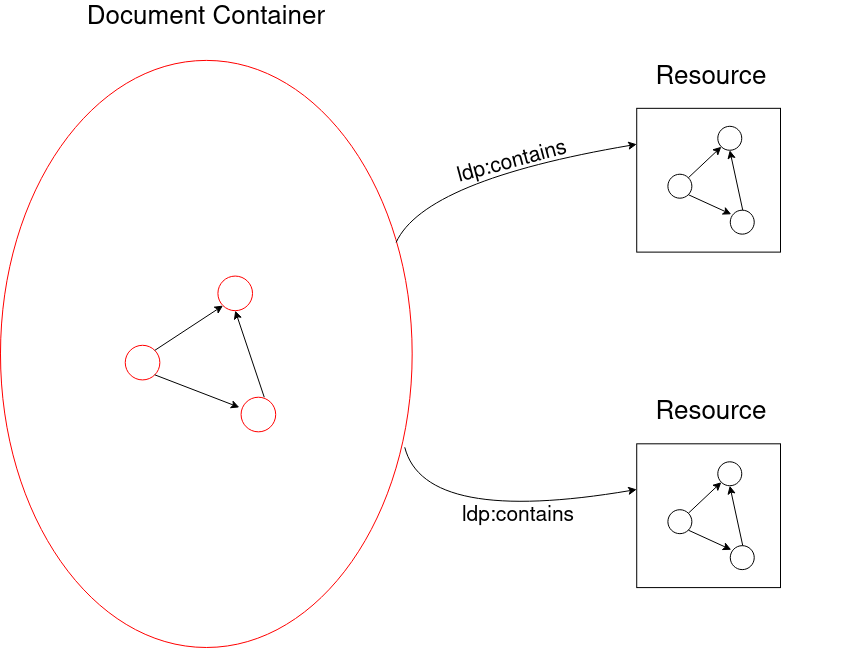
\includegraphics[width=0.60\textwidth]{images/background/ldp-bc.png}}\\
\noindent Direct Containers, or LDP-DCs, are a specialization of a Basic Container. The LDP-DC can make assertions, called membership triples, on resources withing the container. These assertions, which use domain-specific vocabulary, are made as part of the creation process for resources placed in the container. The membership triples do not need to refer to the container resource - these can refer to other resources as well. The figure below illustrates a LDP Basic Container containing movies, and a LDP Direct Container containing documents (images, movies, ..) where the actor is depicted, illustrated through the predicate \texttt{foaf:depicton}. \\
\phantom{kkk|||}{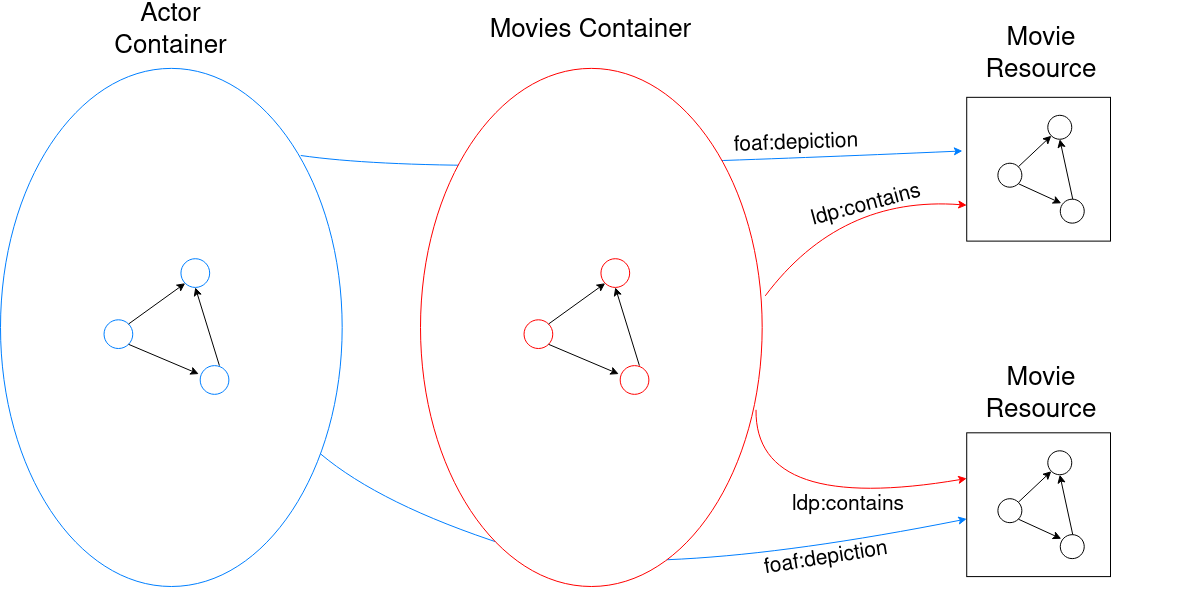
\includegraphics[width=0.9\textwidth]{images/background/ldp-dc.png}}\\

\noindent \textit{Source}: \url{https://www.w3.org/TR/ldp-primer/}
\end{formal}

\newpage
\section{Privacy-Enhancing Technologies}
\label{sec:pets}
\subsection{The need for Privacy-Enhancing Technologies}
The concept of privacy has been around for a long time. Even in the 14th century already, cases were brought before court for eavesdropping and opening letters \citep{privacy-history}. Initially, it was more understood in the context of being let alone, especially in one's house or personal properties. Since the dawn of the information age after the Second World War, the concept started to shift more towards privacy in the context of personal information and publications on the topic started to appear. The definition did not change much however, remaining very similar to the one introduced in 1891 by Warren and Brandeis \citep{privacy-history}:
\begin{quote}{Samuel Warren, Louis Brandeis}
    Privacy is described as a right to be let alone and a right of each individual  to  determine,  under  ordinary  circumstances,  what  his  or  her  thoughts, sentiments, and emotions shall be when in communication with others.
\end{quote}
\todo{Compare with definition of privacy in introduction to PETs, compare inward and outward definition}
\noindent The ubiquity of personal data collection in recent years has strengthened privacy concerns. Especially since the Web has become extremely centralized, with only six companies accounting for 43\% of global internet traffic \citep{internet-report}, there has been a growing demand for technologies that help protect user privacy.

Not only from the data subject's perspective is there a growing concern for data privacy. With the introduction of the \gls{GDPR} in 2018, companies have a legal obligation to take care of user data, especially if it is sensitive. This clashes with the rise of the Saas/PaaS business models, where companies outsource data storage and management. However, this is not always possible and comes with risks. If a Data Processor (a third party that processes data on behalf of a Data Controller) leaks data, the Data Controller risks violating the user's trust (and legal sanctions). \todo{Optional reading or subsection about GDPR to explain basics and terminology?}

In both cases, Privacy-Enhancing Technologies play a big role in reducing the risk of data leaks and preserving user privacy. \citeauthor{pets-handbook} introduced the following definition, which was later adopted by the European Commission\footnote{\url{https://eur-lex.europa.eu/LexUriServ/LexUriServ.do?uri=COM:2007:0228:FIN:EN:PDF}}:
\begin{quote}{\citeauthor{pets-handbook}}
    Privacy-Enhancing Technologies is a system of ICT measures protecting informational privacy by eliminating or minimising personal data thereby preventing unnecessary or unwanted processing of personal data, without the loss of the functionality of the information system.
\end{quote} 
The following sections will introduce a number of widely used \gls{PETs}, some of which will be used in \middleware{}.

\subsection{Data (de-)identification}
\label{sec:data-deid}
The previous section gave an introduction to the concept of privacy. In IT systems, this applies to personal data. But when is data personal? In the context of ePrivacy, the term \textit{\gls{PII}}, is used widely. The term applies to data elements that contain references to attributes that can, either directly or indirectly, disclose someone's identity. A distinction can then be made between three types of data \citep{de-id-taxonomy}:
\begin{itemize}
    \item \textbf{Direct identifiers}: data attributes that directly identify an individual. Examples are national identification numbers, home addresses, e-mail addresses, full names, etc.
    \item \textbf{Indirect identifiers}: data attributes that can be combined with other data attributes to identify an individual, but do not disclose an identity on their own. Examples are birth dates, family names, IP addresses etc.
    \item \textbf{Non-PII elements}: data attributes that contain no reference at all to a person's identity.
\end{itemize}
\noindent \citeauthor{privacy-design-strategies} notes that much like security, privacy is a core property of software systems, and is heavily architecture-dependent. It is therefore of paramount importance that privacy considerations are taken into account from the outset and through the whole development cycle. This design philosophy is named \textit{privacy by design} and it is one of the requirements listed in the GDPR. For regular software design, software developers have used software design patterns to solve common architectural problems. Likewise, \citet{privacy-design-strategies} and \citet{de-id-taxonomy} propose a number of \textit{privacy design strategies}.

\subsection{Transformation-based Approaches}
\label{sec:transformation-approaches}
Transformation-based approaches are approaches that modify datasets in a uniform way, such that the resulting dataset contains less \gls{PII}. Since data transformations \textit{modify} the dataset, it is important to note that this has an impact on the utility of the data. Some transformations may be more powerful at anonymizing the data, but at the same time make the data less valuable or even unusable. A balance must be struck between data privacy and utility, where the choice for a certain data transformation is very context-dependent. This section introduces a number of data transformations.

For an overview of common architectural tactics for data de-identification, we look at the literature study by \citeauthor{de-id-taxonomy}. This study includes 163 investigated articles and builds a taxonomy for data de-identification architectural tactics, mostly consisting of transformation-based approaches. Table \ref{table:de-id-taxonomy} presents their proposed data transformation tactics.
\newpage
\begin{table}[H]
\begin{center}
\begin{tabulary}{\textwidth}{p{0.17\textwidth}p{0.83\textwidth}}
\textbf{Tactic name} & \textbf{Description}                                                                                                                                                          \\ \hline
Remove               & The targeted and deliberate omission of PII from the data record or data set.                                                                                                 \\
Select / Filter      & Same as Remove applied to a copy of the data while keeping the original data.                                                                                                 \\
Transform            & The application of a holistic transformation (not targeted on PII elements only) on data elements that is destructive in terms of ability to distinguish these data elements. \\
Mask                 & Overwriting data elements with other values for the purpose of obfuscating the content.                                                                                       \\
Encrypt              & Using cryptographic means to encode the PII attribute values / records / datasets.                                                                                            \\
Randomize            & Tactics that involve the modification of PII attribute values/records by injecting artificial random elements.                                                                \\
Aggregate            & Generalize, combine and group data elements.                                                                                                                                  \\
Blur                 & Reduce the accuracy of the data so that distinguishing characteristics become indiscernible.                                                                                  \\
Pseudonym            & The systematic replacement of direct identifiers with surrogates, whereby the mapping between surrogate and identity is kept separately.                                      \\
Placeholder          & The systematic replacement of direct identifiers with a surrogate that is the same for all members of the population.                                                         \\
Interchange          & The targeted mingling of data elements across members of the population.                                                                                                      \\
Synthetic            & The replacement of data elements with a synthetic placeholder which is a constructed representation specifically aimed at conveying discriminatory features.                 
\end{tabulary}
\caption{Overview of architectural tactics involving data transformations, by \citet{de-id-taxonomy}}
\label{table:de-id-taxonomy}
\end{center}
\end{table}

\subsection{Encrypted Database Systems}\todo{Can I just import table like this (plagiarism/copyright)?}\todo{Do generalisations, such as going from city to province, fall under aggregate?}
Encrypted Database Systems are database systems that store encrypted data, while maintaining some functionality. It is a vast research field, with \citet{sok-cryptdb} being a formative work. The need for encrypted database systems arises from the rise of the PaaS\footnote{Platform-as-a-Service} model, whereby software and database deployment is outsourced to third parties such as Amazon Web Services and others. \todo{Finish paragraph, explain things like leakage}

Many types of encryption exist for these database systems, ranging from very secure to less secure, but in turn providing more functionality. Popular encryption schemes, sorted from least to most leakage, are \citep{cryptdice}:
\begin{itemize}
    \item \textbf{Random/probabilistic encryption}: Random encryption is an encryption scheme in which encrypting the same plaintext results in a different ciphertext. This is usually achieved by making use of the AES encryption scheme, and using a randomly generated Initialization Vector (IV). This scheme provides the strongest data protection, but it offers no useful operations on the data.
    \item \textbf{Deterministic encryption}: Deterministic encryption works similar to random encryption, but now the IV is kept constant. This results in a scheme which gives the same ciphertext for the same plaintext input. This is less secure, but allows for equality comparisons.
    \item \textbf{Order-preserving encryption}: In the order-preserving encryption scheme, the order relationship between plaintext is preserved in the ciphertext. Therefore, it is possible to do order-comparisons between encrypted data elements, allowing functionality such as range queries.
    \item \textbf{Order-revealing encryption}: Order-revealing encryption is an outdated form of order-preserving encryption. Its usage is discouraged, since it has a larger leakage then order-revealing encryption while providing the same level of functionality. \todo{Add citation here}
\end{itemize}
A new type of encryption scheme that has recently started to become popular is \textit{homomorphic encryption}: it allows processing on encrypted data by supporting mathematical operations on the encrypted data, such as multiplication and addition. It has become popular over the last decade, with \citet{fhe} being a breakthrough work and Google recently releasing a open-source library\footnote{\url{https://github.com/google/fully-homomorphic-encryption}} supporting fully homomorphic encryption. While Somewhat Homomorphic Encryption already has practical applications, this is less the case for Fully Homomorphic Encryption, with the main hurdle being that it is very computationally intensive.
\begin{itemize}
    \item \textbf{Somewhat Homomorphic Encryption}: Somewhat homomorphic encryption schemes, also called partially homomorphic encryption schemes, are homomorphic encryption schemes that support either addition or multiplication, but not both \citep{she}. An example of a additive homomorphic encryption scheme is the Paillier Cryptosystem \citep{paillier}. A widely used multiplicative homomorphic encryption scheme is the ElGamal CryptoSystem \citep{elgamal}.
    \item \textbf{Fully Homomorphic Encryption}: Fully homomorphic encryption schemes are homomorphic encryption schemes that support both addition and multiplication on encrypted data. This is incredibly powerful, since any function can be represented as a circuit consisting of multiplication and addition gates. It can, theoretically, thus compute any function over encrypted data. However, it is still too computationally intensive for a number of practical applications \citep{he-practical, pragmatic-mpc}. Despite that hurdle it remains a promising technology, allowing applications such as encrypted search queries \citep{fhe}, and every year more efficient implementations are proposed.
\end{itemize}
\subsection{Other Approaches}
\subsubsection{Secure Multi-Party Computation}
\label{sec:mpc}
\gls{MPC} is an exciting research field that has seen a large amount of research over the last few decades, while the techniques and modern computers have only recently evolved enough to allow practical applications. It is a technique that allows any number of parties to secretly compute any function over some encrypted input data, while only revealing the requested output to the parties. The basic techniques for Multi-Party Computation stem from a groundbreaking paper by \citet{yao} (for two-party computation), which was later extended to the multi-party case by \citet{mpc}.

\gls{MPC} has a somewhat unusual security model, since the adversary can be a party to the computation instead of being an outsider. The adversary model thus considers some adversarial entity, which manages to exert control over a subset of the parties partaking in the computation. Such a controlled party is called \textit{corrupted}. Often, a \textit{monolithic adversary} is considered: if there are multiple corrupted parties, it is assumed they work together \citep{mpc-good-practice}. When an adversary controls multiple corrupted parties, several \textit{corruptions strategies} are possible \citep{secure-mpc}. In the \textit{static corruption model}, the set of corrupted parties is fixed from the onset and does not change during execution of the protocol. In the \textit{adaptive corruption model}, the adversary can corrupt parties during the execution, but once a party has been corrupted it remains corrupted until the end of the protocol. Finally, there is the \textit{proactive security model} \citep{sec-transient-failures}, where corrupted parties can become honest again (for example, because a breach has been detected and the systems are recovered).\todo{Too detailed?}

Of course, many protocols exist for facilitating computation between multiple parties, even HTTP would support that. The goal of \gls{MPC} is to provide a \textit{secure} protocol. Often, the \textit{real-ideal}\footnote{In the real-ideal security definition, an adversary can not harm the real protocol more than what would be possible in an ideal protocol \citep{mpc}} definition of security is taken to define when such a system is secure. However, this does not provide many practical guidelines. \citet{secure-mpc} lists a number of minimal (but not exhaustive) requirements, which every secure protocol should fulfill:

\begin{quote}{\citet[p.2]{secure-mpc}}
\begin{enumerate}
    \item \textbf{Privacy}: No party should learn anything more than its prescribed output.
    \item \textbf{Correctness}: Each party is guaranteed that the output it receives is correct.
    \item \textbf{Independence of Inputs}: Corrupted parties must choose their inputs independently of the honest parties' inputs.
    \item \textbf{Guaranteed Output Delivery}: Corrupted parties should not be able to prevent honest parties from receiving their output.
    \item \textbf{Fairness}: Corrupted parties should receive their outputs if and only if the honest parties also receive their outputs.
\end{enumerate}
\end{quote}
The actual computation, then, is usually based on something called a \textit{garbled circuit}, introduced by \citeauthor{yao}\todo{add citation for garbled circuits}. The function to be computed is represented as a boolean circuit where the gates are encrypted. \todo{source}The explanation of the complete protocol is out of the scope for this thesis, but it is described in \citet{secure-mpc, pragmatic-mpc} and uses techniques such as Oblivious Transfer\todo{cite}. For some use-cases, generic \gls{MPC} protocols may not be the most efficient and specific protocols that are much faster may exist. A very common example is Private Set Intersection\todo{cite, add acronym}.

\subsubsection{Differential Privacy \& \textit{k}-Anonymity}
Differential privacy and \textit{k}-Anonymity are both types of \textit{statistical} privacy. 

In differential privacy, participating in a database does not substantially increase the risk to the user's privacy \citep{diff-privacy}. \todo{Look later at this paper, it provides some references to proofs that non-interactive (ie data transformations) work less well than interactive approaches, because at the time of the sanitization the future utility is not always known yet. Then discuss that statistical methods cannot be used since we only have data from one user.} This definition follows from \citeauthor{diff-privacy}'s impossibility proof of absolute disclosure prevention. She proved that even if a database has very little information (such as the average height of a person for every country), even that information can lead to a privacy breach in the presence of side information. Imagine that a person's height is sensitive information, and that it is known that Alice's height is 2cm less than the average height. Then the database containing average heights discloses Alice's height, leading to a privacy breach. Because this is impossible to circumvent, \citeauthor{Dwork} introduces the relative notion: a disclosure is just as likely whether the individual takes part in the database or not. In short, the technique works by adding specifically chosen random noise to the answer of a query, to statistically provide the \textit{$\epsilon$}-differential privacy guarantees. A more rigorous explanation can be found in \citet[p9-11]{diff-privacy}.

\textit{k}-Anonymity was introduced by \citet{k-anonymity}, who defined it in terms of de-identifying persons from so-called \textit{quasi-identifiers} (i.e. indirect identifiers) in released data sets. \citet{demographics-identify-unique} notes that 53\% of the U.S. population can be uniquely identified with only the following attributes: place, gender and date of birth. In this context, it is very difficult to correctly identify indirect identifiers, since it is not known beforehand with which data this can be combined to determine unique identities. If a dataset is \textit{k}-anonymous, however, it is impossible (even when combining with another dataset), to uniquely identify individuals. A data release is \textit{k}-anonymous if "the information for each person contained in the release cannot be distinguished from at least \textit{k}-1 individuals whose information also appears in the release" \citep{k-anonymity}. Thus, every unique combination of identifiers maps to at least \textit{k} individuals, making individual identification unlikely\footnote{There exist attacks on \textit{k}-anonymity, but most can be resisted by following the accompanying policies stipulated in \citet{k-anonymity}.}.

\subsection{Related works}\todo{Is this section useful? Or does the general text already give enough references to related works?}
\noindent \textbf{CryptDB} \citep{cryptdb} is a seminal work in the research field of encrypted database systems. It is a SQL database that allows queries over encrypted data. Its main contributions are the demonstration of two new techniques, \textit{adjustable query-based encryption} and \textit{encryption key chaining}. 

Adjustable query-based encryption is a technique that dynamically adapts the the encryption scheme of columns based on queries: it automatically selects the highest possible security given the queries that need to be executed on that column. It does this in a two-fold manner. Firstly, different columns (and tables) have different encryption keys, so that the encryption level can be varied on data fields (some columns might be more sensitive and thus require stronger encryption). Secondly, CryptDB encrypts columns in an \textit{onion}: when the database is initialized, every column is encrypted several times, each time with a stronger encryption mechanism. When a query is then executed against a column whose strong encryption scheme is not compatible with the query, layers are removed until a compatible encryption scheme is reached. 

Encryption key chaining then, is a method to cryptographically enforce access control policies. In CryptDB, principals (either users or groups of users) all have their own key. \citeauthor{cryptdb} developed a novel way to encrypt data such that only the correct principals have access to the data, by making use of both symmetric and asymmetric keys: they use symmetric keys when both users are online, so an interim key can be stored in memory, or asymmetric encryption when one of the users is not online. This strikes a balance between security (only current keys of online users can be leaked in case of an attack) and performance (as symmetric encryption is much more performant). The technique itself requires some background information and can thus be found in the paper itself.\todo{This paragraph does not bring over the idea well, so should be rewritten later}\\

\noindent \textbf{DataBlinder}, by \citet{datablinder}, presents ... \todo{Write more about related works}\\

\noindent \textbf{Cryptdice} \citep{cryptdice} illustrate ...\\

\noindent \textbf{Secure Multi-Party Computation} \citep{secure-mpc} gives a good overview of\\


\chapter{Use cases, requirements and system overview}
\label{cha:solution-overview}
This chapter starts by introducing three use cases that illustrate the problem statement. To illustrate the problems that occur in these use cases more clearly, a generic data aggregation architecture is subsequently presented. This architecture will highlight a number of problems that currently exist and, together with the use cases, will serve to derive a number of 
requirements and an adversary model.

Thereupon, based on all these requirements, a high-level overview of the middleware system is given. This middleware, called the Middleware for Aggregation Security in Solid (MASS), is partially implemented as a prototype on top op the \acrlong{CSS}. The next chapters then start by studying a number of \gls{PETs} in order to determine which technologies are usable in \middleware{}. The chapters following this finally discuss the components of the solution in detail.

\section{Use cases: health and finance}
\label{sec:usecases}
This section describes three use cases which highlight the need for a middleware for secure and protected data aggregation in Solid. These use cases illustrate the complexities and challenges that come with developing such a middleware, and will serve as a guide throughout the development of the solution. The use cases are located in the domains of health and finance, since these traditionally come with sensitive data. Furthermore, data in these domains can also lead to interesting insights, forming ideal candidates for data aggregation.

\subsection{Exercise data}
\label{usecase:ex-data}
In this use case a user stores her exercise data, from an application such as Strava, on her Solid pod. She wishes to export this data to a ranking board application to see which of her friends runs the fastest. However, she does not wish to share her exact heart rate since this is sensitive data and might leak information about her fitness. This data is stored in the TCX file format\footnote{Schema: \url{https://www8.garmin.com/xmlschemas/TrainingCenterDatabasev2.xsd}}. An advantage of this format is that it is supported by popular tools such as Strava and can be imported/exported by exercise trackers such as Garmin devices.

\subsection{Personal finance}
\label{usecase:personal-finance}
This use case describes a scenario wherein a user has stored all his transactions on his Solid pod. He wishes to see some trends and statistics about his spending, and compare this to similar households. An example of such a statistic is ``how much do I spend on groceries every week?''.  However, expenses are very sensitive data, especially when these are exact numbers and store locations. Therefore, the middleware should filter out the most sensitive information yet still receive relevant statistics. This can be done, for example, by removing direct identifiers and perturbing exact spending at individual transactions. For example, for entries of the type ``Bob spent \texteuro 5,82 at Colruyt Leuven on 8/11/2021 16:53'', the user wishes that this is modified into something similar to ``User87532 spent \texteuro 5 at Supermarket on 8/11/2021''. This way, trends in the spending are kept (by perturbing exact amounts to nearby integers, and replacing exact stores with store types). Information such as ``you spent \texteuro 400 in supermarkets this month'' will still be available (and relatively accurate), without giving away exact details. For this use case a custom data format is used, since most standard data schemes for financial information are overly complex for a proof-of-concept.

\subsection{Aggregated view on personal health data streams}
The third use case is taken from one of the SolidLab\footnote{A research project initiated by the Flemish government \citepjournal{solid-flanders}} challenges. Concretely, the challenge \textit{aggregated view on sensitive personal health data streams} is studied\footnote{See \url{https://github.com/SolidLabResearch/Challenges/issues/16}}.

This use case describes a scenario wherein a caretaker wishes to gain insights on all her patients, without knowing exact patient details. These insights are provided through a dashboard, which shows some key statistics about the patient population. Examples of such statistics are average heart rates, average number of steps taken throughout the day, what percentage of the population woke up before 9 am, etc. Of course, the collection and aggregation of such data does not come without issues. Data is derived from activity trackers and IoT sensors, which regularly update data in the user's pod. A secure aggregator must then collect data from all these pods, combine these into aggregate statistics, and write this to a new pod accessible to the caretaker.

\newpage

\section{A generic data aggregation architecture in Solid}
\label{sec:generic-agg-arch}
An aggregation system in Solid will necessarily consist of a number of components, each with their own responsibility. Figure \ref{fig:reference-architecture} illustrates a reference architecture of such a data aggregation system in Solid. 

\begin{figure}[h]
    \centering
    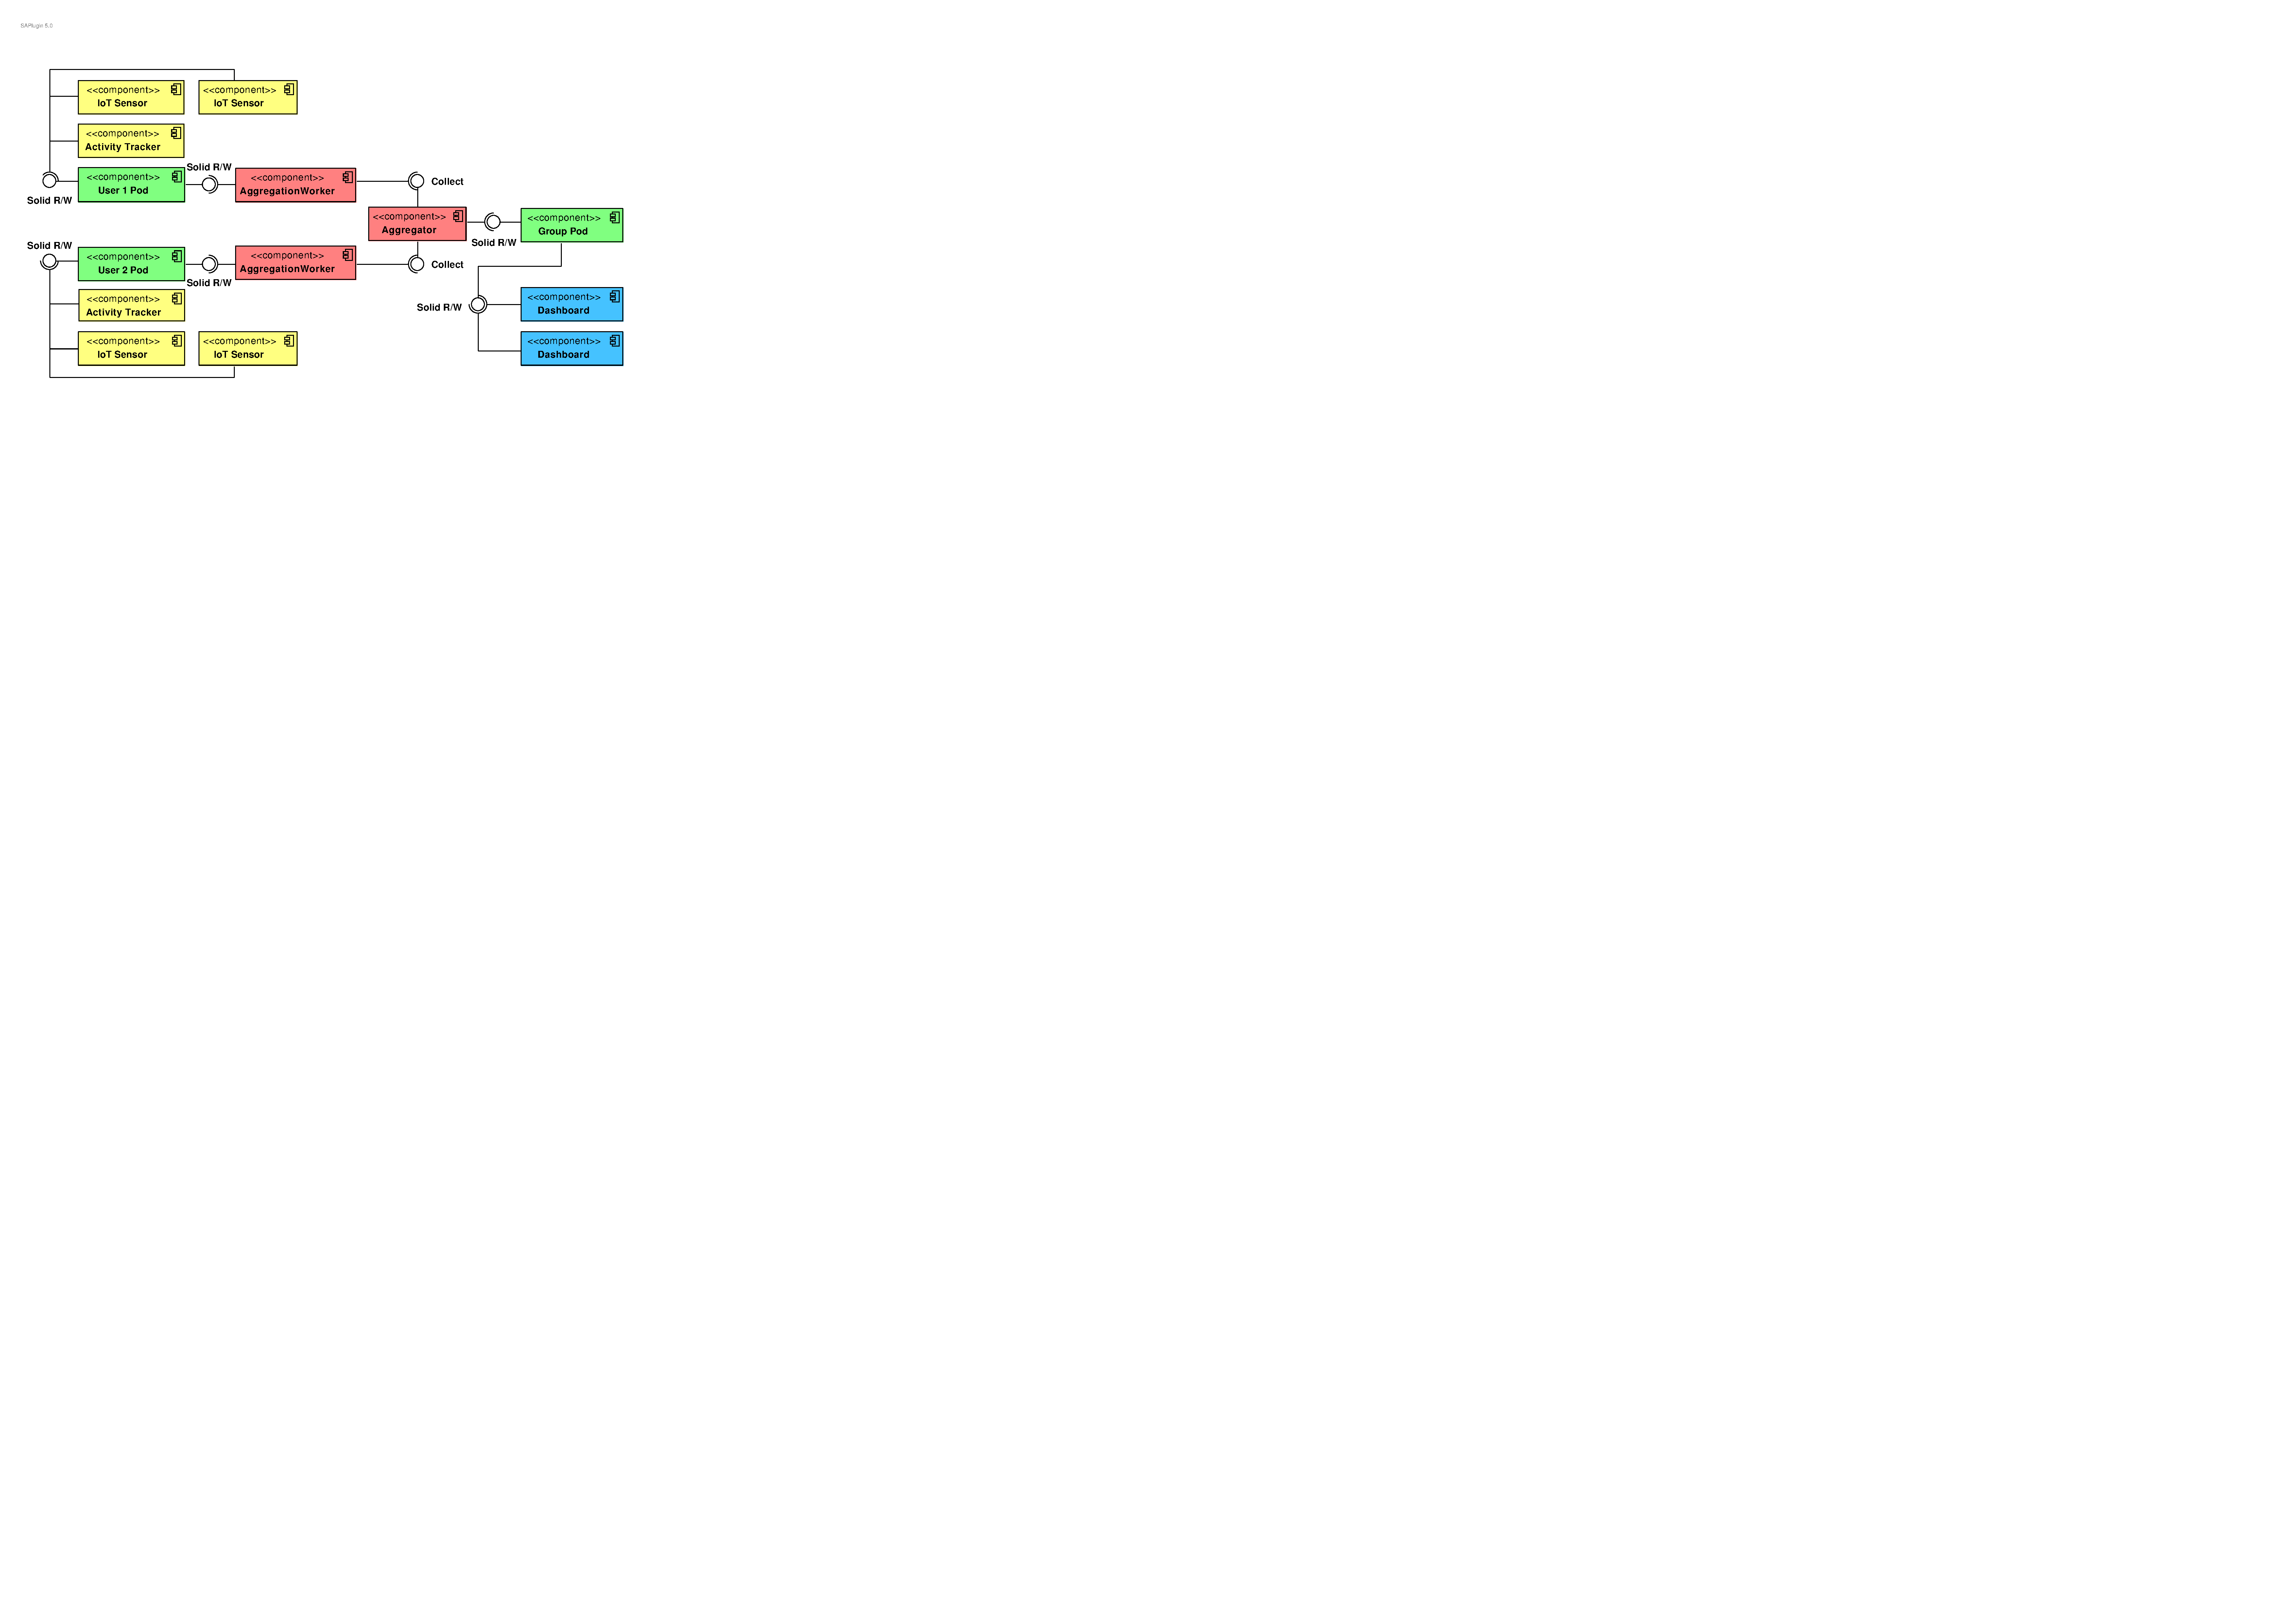
\includegraphics[width=1.0\textwidth]{images/architecture/Reference-Architecture-Aggregator.pdf}
    \caption{Reference architecture for data aggregation in Solid}
    \label{fig:reference-architecture}
\end{figure}

\noindent This reference architecture highlights a number of challenges that make aggregation insecure, unscalable or privacy-invasive. Concretely, the following issues are remarked:

\begin{enumerate}
    \item IoT Sensors and activity trackers are embedded devices that very regularly write data to a Solid pod. As these are resource-constrained devices, those write operations must be very efficient. As section \ref{sec:dpop} explains, the currently used mechanism uses public-key cryptography, which is very computationally expensive.
    \item The aggregator component (illustrated in red on the figure) reads complete resources directly from the user's pod. Privacy-wise, this is unsafe and unnecessary, as not all data present in the resource may be necessary for performing the aggregation. Some method of restricting the data exposed to the aggregator must be devised.
    \item The aggregator component can consist of multiple worker nodes in different networks. Similarly, services can require data from a Solid Pod but also depend on other services that also need access to this data. This is currently not supported in Solid, and existing flows (such as OAuth On-Behalf-Of) impose bottlenecks on the token endpoint. 
    \item Group pods holding data of users from different pod providers are not supported as of yet. This comes with challenges in the authentication domain.
\end{enumerate}

\noindent All of these problems can be mitigated (at least partially) in the domain of the Solid server, which provides the user's pods. A number of improvements here could help alleviate the problems listed above. These problems can be divided in two categories: resource management and authentication management. To solve these problems, a solution will need to consist of two parts: one focused on rendering exposed resources more private, the other focused on improving the authentication mechanism. In the next section, requirements for the needed solution will be derived based on the problems that have been illustrated in this section.

\section{Requirements}
\label{sec:requirements}
This section introduces a number of requirements, based on the use cases and architecture presented in the previous sections. First, functional requirements with a major impact on the architecture are discussed. The second subsection then discusses a number of non-functional requirements. These requirements will help designing an effective solution, and their realization will also be evaluated later.

\subsection{Functional requirements}
\noindent \textbf{Flexibility for the supported data scheme} Solid builds further upon the principles of Linked Data, and Solid servers can store nearly any type of data. As \middleware{} aims to be a general solution, it should work with any type of structured data, i.e., it must provide a way to anonymize \textit{any} type of textually represented structured data. Thus, flexibility for the supported data scheme is an essential part of \middleware{}. Concretely, \middleware{} should not hardcode any supported data schemes nor which \gls{PETs} should be applied to them: these should be able to be plugged in flexibly and selected automatically, to ensure that any data scheme can be supported. This provides a technical challenge, as a sufficient level of abstraction must be developed to be able to support any data scheme, while ensuring that the leakage requirements are not violated. \\

\noindent \textbf{Automatically select \gls{PETs}} Different applications may be trusted differently, just as different data types may contain more or less sensitive data elements. An important aspect to solve is thus being able to distinguish different \textit{privacy levels}: required levels of anonymization. \middleware{} must therefore not only be able to adapt to different data schemes, but must also support different privacy levels for every data scheme. The selected PET is highly dependent on the data scheme and required level of privacy, therefore \middleware{} must automatically select \gls{PETs} based on the data type of the requested resource and the requested privacy level. This privacy level must be automatically determined by \middleware{} based on the context of the request, i.e., what data type is requested and by which application. \\

\noindent \textbf{Extensibility} The Solid project is still very much a work in progress. This implies that the specification will likely be modified many times in the future, and additional features will be added. If \middleware{} wants to successfully keep interacting with Solid servers, the architecture should be designed such that it can easily be extended in order to support newly released features and modifications. \\

\noindent \textbf{Decentralized access token delegation} As aggregators may consists of multiple worker nodes, or may be dependent of other services, the middleware solution must also enable a mechanism for decentralized access token delegation. In other words, an application must be able to delegate its access token without having to request a new token at the token endpoint. The user should explicitly give access for this.

\subsection{Non-functional requirements}
\textbf{Intuitive to use} Solid aims to become the de facto standard for web applications in the future. Consequently, it must be intuitive for non-technical users to use this technology. There can be no technical jargon, and it must be easy to set-up. Since \middleware{} aims to follow this philosophy, the proposed solution must be intuitive to use for non-technical users.  Concretely, this means that it should be opaque to the users which concrete PET is applied for which use case. On that account, a number of \textit{privacy levels} should be created and presented to the user in a simple manner: a higher privacy level means more data protection but less utility. The user will then be able to select between a number of privacy levels, without needing to understand the technical details behind the scenes. Examples of concrete transformations can be given, to make the effects of selecting a certain level more comprehensible. \\

\noindent \textbf{Testability} Since \middleware{} operates so dynamically, there is a lot of opportunity for bugs to sneak in that will go unnoticed. Some bugs may only appear under the presence of a specific combination of transformations in the configuration files. Therefore, testability is an important aspect. Increased testability gives stronger guarantees of the correct behavior of \middleware{}, which is essential in the context of a privacy-enhancing technology. \\

\noindent \textbf{Minimal overhead} Since \middleware{} operates as a middleware, it will be called on every resource request. The overhead associated with this should be minimized, such that the used Solid server does not become unusable due to running the middleware.

\section{Adversary model}
\label{sec:attacker-model}
The attacker model considered in the design and development of \middleware{} is an honest-but-curious attacker, i.e., an attacker that follows the protocol but will try to read as much information as possible within this confinement. This model is considered since the middleware handles the case of untrusted aggregators and applications. Untrusted in this case means that the user wishes to use the aggregator or application, but wants to minimize the amount of data exposed to it. Thus, the adversary is a Solid application to which the user grants access and that can thus access any data to which the \gls{ACL}s give it access. However, there is no fine-grained privacy control, i.e., on the level of a single resource. 

It is important to note the goal of \middleware{} in terms of disclosure prevention here. As will be explained in section \ref{sec:statistical-privacy}, many \gls{PETs} try to prevent identity disclosure (in datasets containing data from many different users). However, since every Solid pod is linked to a WebID, the main goal of this middleware is to prevent attribute disclosure. Accordingly, the attackers considered try to gain knowledge of \textit{data attributes}. Handling identity disclosure is also an important aspect of a privacy-aware software system, but in the case of data aggregators this must be handled by the aggregators themselves.

\section{System overview}
To solve the problems and fulfill the requirements stipulated above, \middleware{} consists of two main components. The first component is called \textit{privacy filters} and focuses on improving data privacy for data exposed to aggregators (or other applications). The second component is an implementation of macaroons in Solid, i.e. a new access token mechanism. This mechanism supports decentralized delegation, group vaults, and is computationally very efficient (to support data writes by IoT sensors, ...).

Privacy filters are a mechanism to dynamically modify requested resources by restricting sensitive data attributes. When a resource is requested for aggregation, it often contains a lot of unnecessary and private information. To resolve this, privacy filters dynamically modify certain attributes of the resource. This is realized by loading a number of configuration files on to the server (or the user's pod), which describe what \textit{privacy tactics} ought to be applied to a certain data scheme, for a given \textit{privacy level}. Privacy levels are a granular way to select how much to trust a certain application or aggregator (i.e., how private should the resource be rendered). The next chapter studies a number of \gls{PETs} to determine which are usable in \middleware{}. Privacy filters are then discussed in detail in chapter \ref{cha:privacy-filters}. 

To alleviate the authentication and authorization problems that come with data aggregation in Solid, this dissertation further investigates the use of macaroons in Solid. Some background information on macaroons has been given in section \ref{sec:macaroons}. Macaroons support decentralized delegation out-of-the-box, and also support \textit{caveats} (requirements which must be fulfilled for a token to be valid), as well as third-party attestations. These properties can improve aggregation security, for example by embedding the required privacy level inside the access token, as well as providing a natural mechanism for realizing group vault using the third-party attestations. Lastly, macaroons use \acrlong{HMAC} instead of public-key cryptography. This creates performance improvements that enable IoT devices or activity trackers to more efficiently write to Solid pods. The integration of macaroons in Solid is discussed in detail in chapter \ref{cha:macaroons-solid}. The combination of these two components can enable better and more secure data aggregation in Solid. Figure \ref{fig:aggregation-flow} illustrates more concretely the flow of data aggregation using these two new mechanisms.

\begin{sidewaysfigure}[h]
    \centering
    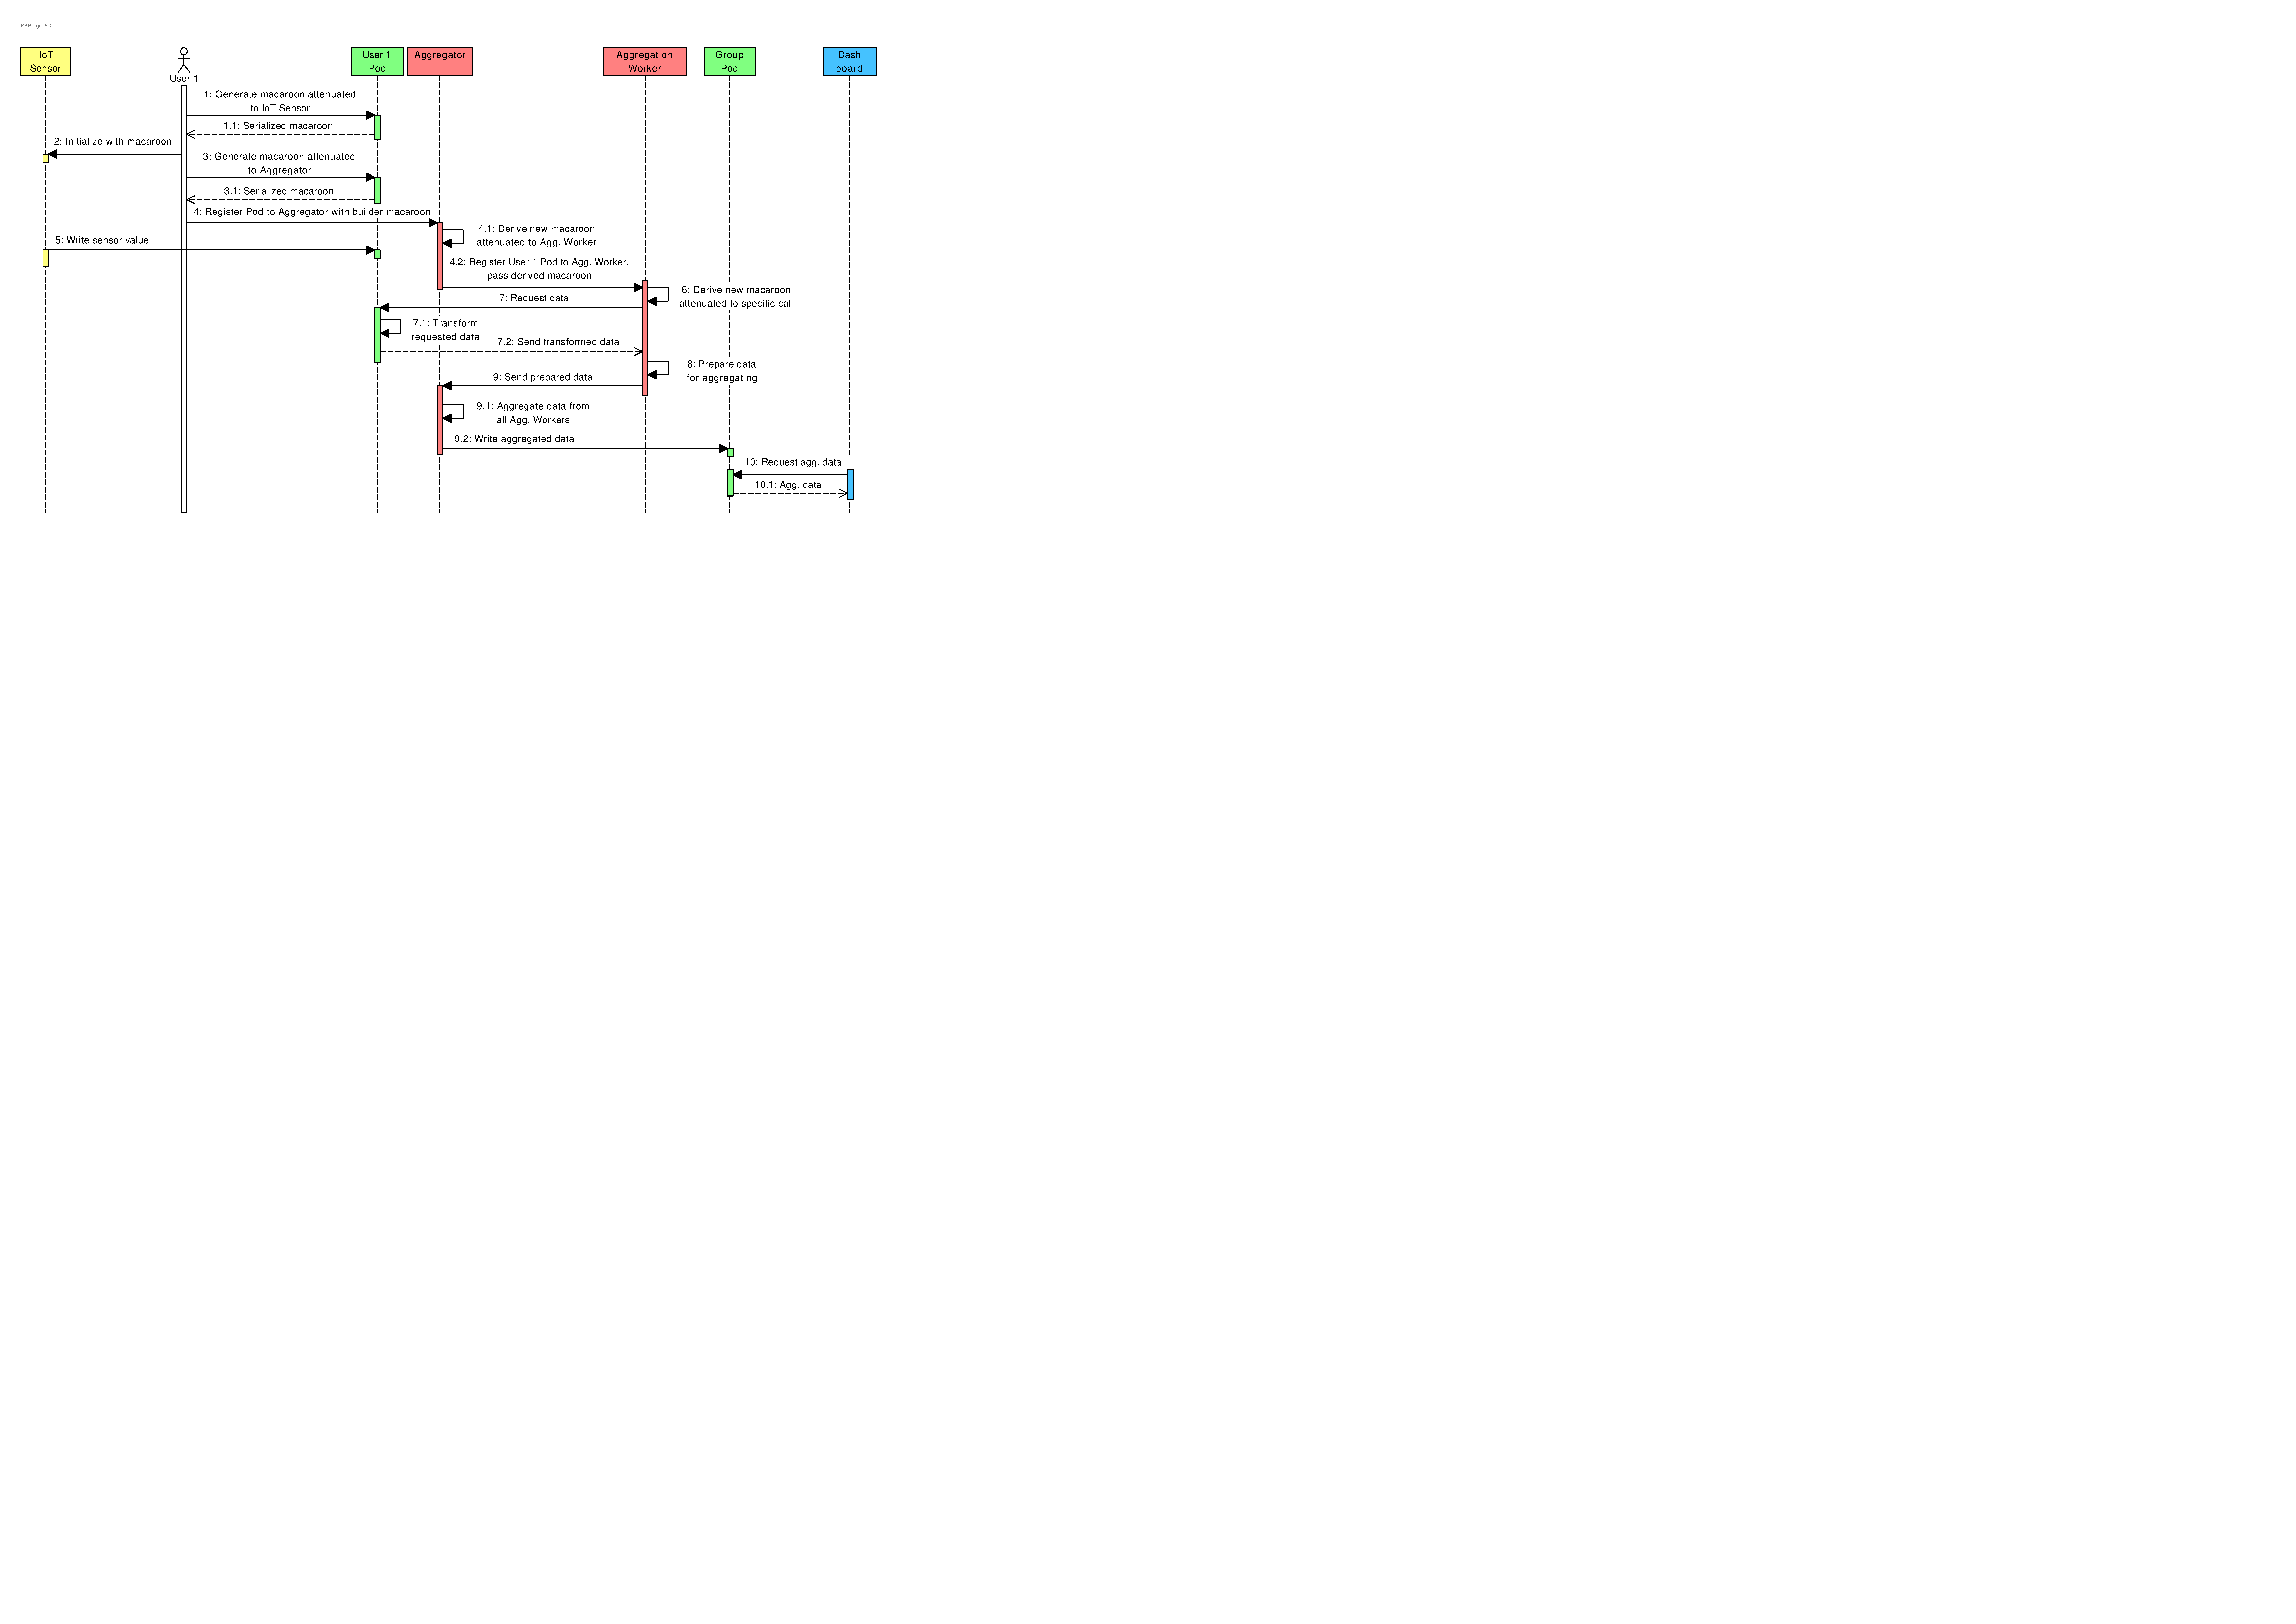
\includegraphics[width=1.0\textwidth]{images/architecture/InteractionDiagram-Aggregation-flow.pdf}
    \caption{Aggregation flow}
    \label{fig:aggregation-flow}
\end{sidewaysfigure}

\chapter{Study of Privacy-enhancing Technologies}
\label{cha:analysis}
This chapter studies a wide range of \gls{PETs}, discussing how they work and analyzing whether they are applicable in the context of enhancing data privacy in Solid. As explained in section \ref{sec:outline}, a component for enhancing privacy is first studied and developed. 
This analysis forms the basis for selecting a number of \gls{PETs} that will be supported in the privacy-enhancing component of \middleware{}, the developed aggregation middleware. 

\section{Introduction}
\label{sec:pets}
\subsection{The need for Privacy-Enhancing Technologies}
The concept of privacy has been around for a long time. Even in the 14th century already, cases were brought before court for eavesdropping and opening letters \citep{privacy-history}. Initially, it was more understood in the context of being let alone, especially in one's house or personal properties. Since the dawn of the information age after the Second World War, the concept started to shift more towards privacy in the context of personal information and publications on the topic started to appear. The definition did not change much however, remaining very similar to the one introduced in 1891 by Warren and Brandeis \citep{privacy-history}:
\begin{quote}{Samuel Warren, Louis Brandeis}
    Privacy is described as a right to be let alone and a right of each individual  to  determine,  under  ordinary  circumstances,  what  his  or  her  thoughts, sentiments, and emotions shall be when in communication with others.
\end{quote}
\noindent The ubiquity of personal data collection in recent years has strengthened privacy concerns. Especially since the Web has become extremely centralized, with only six companies accounting for 43\% of global internet traffic \citep{internet-report}, there has been a growing demand for technologies that help protect user privacy.

Not only from the \textit{Data Subject}'s perspective is there a growing concern for data privacy. With the introduction of the \gls{GDPR} in 2018, companies have a legal obligation to take care of user data, especially if it is sensitive. This clashes with the rise of the Saas/PaaS business models, where companies outsource data storage and management. However, this is not always possible and comes with risks. If a \textit{Data Processor}\footnote{Data Subject, Data Processor and Data Controller are roles defined in the \gls{GDPR}. For a concise but correct definition, please refer to \url{https://ec.europa.eu/info/law/law-topic/data-protection/reform/rules-business-and-organisations/obligations/controller-processor/what-data-controller-or-data-processor_en}} (a third party that processes data on behalf of a Data Controller) leaks data, the \textit{Data Controller} risks violating the user's trust (and legal sanctions). \todo{Optional reading or subsection about GDPR to explain basics and terminology?}

In both cases, Privacy-Enhancing Technologies play a big role in reducing the risk of data leaks and preserving user privacy. \citeauthor{pets-handbook} introduced the following definition, which was later adopted by the European Commission\footnote{\url{https://eur-lex.europa.eu/LexUriServ/LexUriServ.do?uri=COM:2007:0228:FIN:EN:PDF}}:
\begin{quote}{\citeauthor{pets-handbook}}
    Privacy-Enhancing Technologies is a system of ICT measures protecting informational privacy by eliminating or minimising personal data thereby preventing unnecessary or unwanted processing of personal data, without the loss of the functionality of the information system.
\end{quote} 
%The rest of this chapter will introduce a number of widely used \gls{PETs}, some of which will be used in \middleware{}.

\subsection{Data (de-)identification}
\label{sec:data-deid}
The previous section gave an introduction to the concept of privacy. In IT systems, this applies to personal data. But when is data personal? In the context of ePrivacy, the term \textit{\gls{PII}}, is used widely. The term applies to data elements that contain references to attributes that can, either directly or indirectly, disclose someone's identity. A distinction can then be made between three types of data \citep{de-id-taxonomy}:
\begin{itemize}
    \item \textbf{Direct identifiers}: data attributes that directly identify an individual. Examples are national identification numbers, home addresses, e-mail addresses, full names, etc.
    \item \textbf{Indirect identifiers}: also called quasi-identifiers, these are data attributes that can be combined with other data attributes to identify an individual, but do not disclose an identity on their own. Examples are birth dates, family names, IP addresses etc.
    \item \textbf{Non-PII elements}: data attributes that contain no reference at all to a person's identity.
\end{itemize}
\noindent \citeauthor{privacy-design-strategies} notes that much like security, privacy is a core property of software systems, and is heavily architecture-dependent. It is therefore of paramount importance that privacy considerations are taken into account from the outset and through the whole development cycle. This design philosophy is named \textit{privacy by design} and it is one of the requirements listed in the GDPR. For regular software design, software developers have used software design patterns to solve common architectural problems. Likewise, \citet{privacy-design-strategies} and \citet{de-id-taxonomy} propose a number of \textit{privacy design strategies}, which will be used extensively.

\section{Transformation-based Approaches}
\label{sec:transformation-approaches}
Transformation-based approaches are approaches that modify datasets in a way such that the resulting dataset contains less \gls{PII}. The transformation-based approaches studied  in this section all happen on a row-by-row basis. Since data transformations \textit{modify} the dataset, it is important to note that this has an impact on the utility of the data. Some transformations may be more powerful at anonymizing the data, but at the same time make the data less valuable or even unusable. A balance must be struck between data privacy and utility, where the choice for a certain data transformation is very context-dependent. This section introduces a number of data transformations.

For an overview of common architectural tactics for data de-identification, we look at a literature study by \citeauthor{de-id-taxonomy}. This study includes 163 investigated articles and builds a taxonomy for data de-identification architectural tactics, mostly consisting of transformation-based approaches. Table \ref{table:de-id-taxonomy} presents their proposed data transformation tactics.

Such transformations seem very usable in the context of a middleware that anonymizes data. They are often fairly simple transformations, that can range in privacy strength and resulting utility. Because these transformations are so dynamic, they are perfect to adapt to different trust levels of applications, allowing more impactful transformations on data sent to applications that are less trusted. Another big advantage of an approach taking advantage of data transformations is that this can be realised statelessly. As the data is sanitized on a row-by-row or record-by-record basis, independently of the other records, there is no need to keep track of state. This heavily simplifies possible architectural designs.
\newpage
\begin{table}[H]
\begin{center}
\begin{tabulary}{\textwidth}{p{0.17\textwidth}p{0.83\textwidth}}
\textbf{Tactic name} & \textbf{Description}                                                                                                                                                          \\ \hline
Remove               & The targeted and deliberate omission of PII from the data record or data set.                                                                                                 \\
Select / Filter      & Same as Remove applied to a copy of the data while keeping the original data.                                                                                                 \\
Transform            & The application of a holistic transformation (not targeted on PII elements only) on data elements that is destructive in terms of ability to distinguish these data elements. \\
Mask                 & Overwriting data elements with other values for the purpose of obfuscating the content.                                                                                       \\
Encrypt              & Using cryptographic means to encode the PII attribute values / records / datasets.                                                                                            \\
Randomize            & Tactics that involve the modification of PII attribute values/records by injecting artificial random elements.                                                                \\
Aggregate            & Generalize, combine and group data elements.                                                                                                                                  \\
Blur                 & Reduce the accuracy of the data so that distinguishing characteristics become indiscernible.                                                                                  \\
Pseudonym            & The systematic replacement of direct identifiers with surrogates, whereby the mapping between surrogate and identity is kept separately.                                      \\
Placeholder          & The systematic replacement of direct identifiers with a surrogate that is the same for all members of the population.                                                         \\
Interchange          & The targeted mingling of data elements across members of the population.                                                                                                      \\
Synthetic            & The replacement of data elements with a synthetic placeholder which is a constructed representation specifically aimed at conveying discriminatory features.                 
\end{tabulary}
\caption{Overview of architectural tactics involving data transformations, by \citet{de-id-taxonomy}}
\label{table:de-id-taxonomy}
\end{center}
\end{table}

\section{Encrypted Database Systems}
\label{sec:enc-db}
\noindent Encrypted Database Systems are database systems that store encrypted data, while maintaining some functionality over this data. It is a vast research field, with \citet{sok-cryptdb} being a formative work. The need for encrypted database systems arises from the rise of the PaaS\footnote{Platform-as-a-Service} model, whereby software and database deployment is outsourced to third parties such as Amazon Web Services and others. Since these cloud platforms store sensitive data (customer data, economically valuable information, ...), it is important for certain users to guarantee that these providers are unable to access their stored data. This is realized by encrypting the data, but this brings along problems. As these databases are often very large, information is retrieved through complex queries. These queries may not support operating on encrypted data by default, so some new techniques are necessary.

Many types of encryption exist for these database systems, ranging from very secure to less secure, but in turn providing more functionality. Popular encryption schemes, sorted from least to most leakage, are \citep{cryptdice}:
\begin{itemize}
    \item \textbf{Random/probabilistic encryption}: Random encryption is an encryption scheme in which encrypting the same plaintext results in a different ciphertext. This is usually achieved by making use of the AES encryption scheme, and using a randomly generated \gls{IV}. This scheme provides the strongest data protection, but it offers no useful operations on the data.
    \item \textbf{Deterministic encryption}: Deterministic encryption works similar to random encryption, but now the \gls{IV} is kept constant. This results in a scheme which gives the same ciphertext for the same plaintext input. This is less secure, but allows for equality comparisons.
    \item \textbf{Order-revealing encryption}: In the order-revealing encryption scheme, the order relationship between plaintext is preserved in the ciphertext. Therefore, it is possible to do order-comparisons between encrypted data elements, allowing functionality such as range queries.
    \item \textbf{Order-preserving encryption}: Order-preserving encryption is an outdated form of order-preserving encryption. Its usage is discouraged, since it has a larger leakage than order-preserving encryption while providing the same level of functionality \citep{stanford-ore}.
\end{itemize}
A new type of encryption scheme that has recently started to become popular is \textit{homomorphic encryption}: it allows processing on encrypted data by supporting mathematical operations on the encrypted data, such as multiplication and addition. It has become popular over the last decade, with \citet{fhe} being a breakthrough work and Google recently releasing an open-source library\footnote{\url{https://github.com/google/fully-homomorphic-encryption}} supporting fully homomorphic encryption. While Somewhat Homomorphic Encryption already has practical applications, this is less the case for Fully Homomorphic Encryption, with the main hurdle being that it is very computationally intensive.
\begin{itemize}
    \item \textbf{Somewhat Homomorphic Encryption}: Somewhat homomorphic encryption schemes, also called partially homomorphic encryption schemes, are homomorphic encryption schemes that support either addition or multiplication, but not both \citep{she}. An example of a additive homomorphic encryption scheme is the Paillier Cryptosystem \citep{paillier}. A widely used multiplicative homomorphic encryption scheme is the ElGamal Cryptosystem \citep{elgamal}.
    \item \textbf{Fully Homomorphic Encryption}: Fully homomorphic encryption schemes are homomorphic encryption schemes that support both addition and multiplication on encrypted data. This is incredibly powerful, since any function can be represented as a circuit consisting of multiplication and addition gates. It can, theoretically, thus compute any function over encrypted data. However, it is still too computationally intensive for a number of practical applications \citep{he-practical, pragmatic-mpc}. Despite that hurdle it remains a promising technology, allowing applications such as encrypted search queries \citep{fhe}, and every year more efficient implementations are proposed.
\end{itemize}

\noindent While Encrypted Database Systems form a very active research domain, their possible applications within Solid are rather limited for a number of reasons. First and foremost, Solid is not a database system and does not provide data with support for queries (at the moment). Instead, data fetched through the Solid protocol is in the form of resources, which map to files on a filesystem. In the future, Solid may support RDF queries on the resources, but since this is rather specialized implementing such a system would also be a complex task. The second and most important point is that these encryption systems are ideal for when a single client needs access to a database. However, this maps badly to Solid's decentralized nature, where multiple clients (which are trusted differently and have different access control rights) access multiple Solid pods. This complicates the encryption possibilities substantially, especially regarding key management. 

Homomorphic encryption does have some interesting properties that would benefit from being researched in the context of Solid. Homomorphic encryption could be used to give some encrypted data to an application that then performs computations on it. In this way, a client application could aggregate data from a number of different pods, performing some calculation on it, and then returning this data to the clients, giving them insights. This scenario is further developed as future work in FW \ref{fw:homomorphic-encryption}. This fits well in the goals of this thesis, but then focused on the software that performs the aggregation instead of the middleware.

\section{Secure Multi-Party Computation}
\label{sec:mpc}
\gls{MPC} is an exciting research field that has seen a large amount of research over the last few decades, while the techniques and modern computers have only recently evolved enough to allow practical applications. It is a technique that allows any number of parties to secretly compute any function over some encrypted input data, while only revealing the requested output to the parties. The basic techniques for Multi-Party Computation stem from a groundbreaking paper by \citet{yao} (for two-party computation), which was later improved to support the multi-party case by \citet{mpc}.

\gls{MPC} has a somewhat unusual security model, since the adversary can be a party to the computation instead of being an outsider. The adversary model thus considers some adversarial entity, which manages to exert control over a subset of the parties partaking in the computation. Such a controlled party is called \textit{corrupted}. Often, a \textit{monolithic adversary} is considered: if there are multiple corrupted parties, it is assumed they work together \citep{mpc-good-practice}. When an adversary controls multiple corrupted parties, several \textit{corruptions strategies} are possible \citep{secure-mpc}. In the \textit{static corruption model}, the set of corrupted parties is fixed from the onset and does not change during execution of the protocol. In the \textit{adaptive corruption model}, the adversary can corrupt parties during the execution, but once a party has been corrupted it remains corrupted until the end of the protocol. Finally, there is the \textit{proactive security model} \citep{sec-transient-failures}, where corrupted parties can become honest again (for example, because a breach has been detected and the systems are recovered).\todo{Too detailed?}

Of course, many protocols exist for facilitating computation between multiple parties, even HTTP would support that. The goal of \gls{MPC} is to provide a \textit{secure} protocol. Often, the \textit{real-ideal}\footnote{In the real-ideal security definition, an adversary can not harm the real protocol more than what would be possible in an ideal protocol \citep{mpc}} definition of security is taken to define when such a system is secure. However, this does not provide many practical guidelines. \citet{secure-mpc} lists a number of minimal (but not exhaustive) requirements, which every secure protocol should fulfill:

\begin{quote}{\citet[p.2]{secure-mpc}}
\begin{enumerate}
    \item \textbf{Privacy}: No party should learn anything more than its prescribed output.
    \item \textbf{Correctness}: Each party is guaranteed that the output it receives is correct.
    \item \textbf{Independence of Inputs}: Corrupted parties must choose their inputs independently of the honest parties' inputs.
    \item \textbf{Guaranteed Output Delivery}: Corrupted parties should not be able to prevent honest parties from receiving their output.
    \item \textbf{Fairness}: Corrupted parties should receive their outputs if and only if the honest parties also receive their outputs.
\end{enumerate}
\end{quote}
The actual computation, then, is usually based on something called a \textit{garbled circuit} \citep{garbled-circuit}. The function to be computed is represented as a boolean circuit whose gates are encrypted. The explanation of the complete protocol is out of scope for this dissertation, but it is described in \citet{secure-mpc, pragmatic-mpc}. For some use-cases, generic \gls{MPC} protocols may not be the most efficient and specific protocols that are much faster may exist. A very common example is Private Set Intersection.

Because of the decentralized nature of \gls{MPC}, this forms a very interesting technique to research in Solid. It could be used to securely compute insights over data stored in multiple pods, without even needing to hand out an encrypted version of the data. Computations are performed on the pods itself, and only \textit{secret shares} are sent out\footnote{A secret share is a part of the data that is indistinguishable from a random string. It is used in \gls{MPC} to perform the computations. When $x$ is a confidential piece of data, you could build two secret shares by generating a random $p$ and handing out $x + p$ and $p$. Only by combining the two secret shares can the original secret $x$ be reconstructed}. While this is very interesting, it also entails a very large extension of the Solid protocol or a Solid server. Moreover, this redefines the concept of a pod, making it also a compute engine instead of just a storage space. This scenario is also considered future research and is elaborated in FW \ref{fw:mpc}.

\section{Differential Privacy \& \textit{k}-Anonymity}
\label{sec:statistical-privacy}
Differential privacy and \textit{k}-Anonymity are both types of \textit{statistical} privacy. 

In differential privacy, \textit{"participating in a database does not substantially increase the risk to the user's privacy"} \citep{diff-privacy}.  This definition follows from \citeauthor{diff-privacy}'s impossibility proof of absolute disclosure prevention. She proved that even if a database has very little information (such as the average height of a person for every country), even that information can lead to a privacy breach in the presence of side information. Imagine that a person's height is sensitive information, and that it is known that Alice's height is 2cm less than the average height. Then the database containing average heights discloses Alice's height, leading to a privacy breach. Because this is impossible to circumvent, \citeauthor{diff-privacy} introduces the relative notion: a disclosure is just as likely whether the individual takes part in the database or not. In short, the technique works by adding specifically chosen random noise to the answer of a query, to statistically provide the \textit{$\epsilon$}-differential privacy guarantees. A more rigorous explanation can be found in \citet[p9-11]{diff-privacy}.

\textit{k}-Anonymity was introduced by \citet{k-anonymity}, who defined it in terms of de-identifying persons from so-called \textit{quasi-identifiers} (i.e. indirect identifiers) in released data sets. \citet{demographics-identify-unique} notes that 53\% of the U.S. population can be uniquely identified with only the following attributes: place, gender and date of birth. In this context, it is very difficult to correctly identify indirect identifiers, since it is not known beforehand with which data this can be combined to determine unique identities. If a dataset is \textit{k}-anonymous, however, it is very hard to uniquely identify individuals (given that no other dataset is released - see footnote). A data release is \textit{k}-anonymous if "the information for each person contained in the release cannot be distinguished from at least \textit{k}-1 individuals whose information also appears in the release" \citep{k-anonymity}. Thus, every unique combination of identifiers maps to at least \textit{k} individuals, making individual identification unlikely\footnote{There exist attacks on \textit{k}-anonymity, but most can be resisted by following the accompanying policies stipulated in \citet{k-anonymity}. Most of these attacks stem from the fact that $k$-Anonymity does not compose: combining multiple $k$-Anonymous datasets does not lead to a combined dataset that is also $k$-Anonymous.}.

While both technologies are very interesting, there are a number of crucial aspects that stop them from being usable in the privacy-enhancing middleware this thesis aims to develop. First of all, both methods are applicable in datasets with \textit{multiple} users. There is no point in using these methods on data originating from a single user. For differential privacy, this is because it is defined as your participation in the database having a negligible impact (defined by $\epsilon$). However, when the database only consists of records belonging to a single user, this is impossible. On the other hand, \textit{k}-Anonymity lacks that it focuses on a different aspect than what the middleware tries to achieve. This is because \textit{k}-Anonymity focuses on preventing \textit{identity disclosure}, while in the middleware itself the goals are to lower the risks of \textit{attribute disclosure}. However, \textit{k}-Anonymity may be an interesting approach to prevent identity disclosure on an aggregation system (i.e. the component that collects data across many pods).

\section{Attribute-based Encryption}
\Gls{ABE} is an encryption scheme that was introduced by \citet*{fuzzy-ibe}. In their paper, the authors developed a new type of \gls{IBE}. Traditional \gls{IBE} systems typically use a single string to represent a user's identity; \citeauthor*{fuzzy-ibe} developed a scheme where the identity is not represented by a string but by a set of descriptive attributes. In their scheme, encrypting documents happens with a set of required attributes included. Decryption can then only happen by users whose identity contains all the attributes (or, where there is a big enough set overlap, in their original scheme). However, \citeauthor*{fuzzy-ibe}'s development focused mostly on using \gls{IBE} with biometric identities. A number of follow-up papers extended this idea to make it more suitable for \gls{ABE}, using systems such as \gls{KP-ABE} and \gls{CP-ABE}.

\citet{kp-abe} extends the original paper with \gls{KP-ABE} and makes it more suitable for fine-grained access control. They do this by introducing a new access structure based on a tree consisting of \texttt{AND} and \texttt{OR} gates\footnote{Actually, the tree consists of nodes that act as threshold gates. \texttt{AND} gates are realised as n-out-of-n threshold gates, while \texttt{OR} gates are realised as 1-out-of-n threshold gates}, and the leaves containing attributes. Decryption of the message is then allowed when the attributes satisfy the tree. This access structure, called the policy, is stored in the private key. In the original model, \textit{all} attributes had to match approximately (within the predefined set distance), so this new access structure is much more expressive. \Gls{KP-ABE} associates the ciphertexts with these descriptive attributes, and the user's keys with the policy.

\begin{figure}[h]
\centering
\tikzset{every tree node/.style={minimum width=2em,draw,sibling distance=1em,rectangle,rounded corners,align=center},
         blank/.style={draw=none},
         edge from parent/.style=
         {draw,edge from parent path={(\tikzparentnode) -- (\tikzchildnode)}},
         level distance=1.5cm}
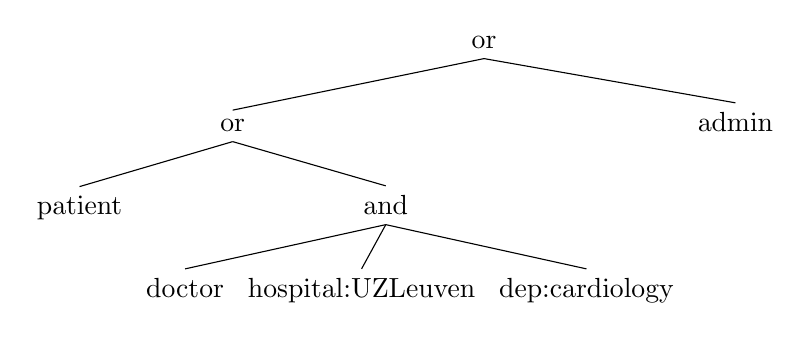
\begin{tikzpicture}
\Tree
[.or     
    [.or 
    \edge[]; [.patient ]
    \edge[]; [.and
             \edge[]; {doctor}
             \edge[]; {hospital:UZLeuven}
             \edge[]; {dep:cardiology}
         ]
    ]
    [.admin ]
]
\end{tikzpicture}
\caption{Example \acrshort{ABE} policy}
\end{figure}

\noindent This scheme works similar to secret sharing schemes, where a number of parties (respectively, attributes) must collude to be able to reconstruct the secret. The main difference is that secret sharing allows cooperation between different parties, but \gls{KP-ABE} does not. If this were allowed, some security requirements could be bypassed. This property is called \textit{collusion resistance}, and is an essential property of \gls{ABE} systems \citep{cp-abe}. 

As an example, take the case of government health data that is encrypted with the attributes \texttt{government} \texttt{AND} \texttt{health}. You would not want a government worker with attribute \texttt{government} be able to collude with a nurse with attribute \texttt{health} to decrypt this data.

\acrlong{CP-ABE} then, is introduced by \citet{cp-abe}. \Gls{CP-ABE} reverses the situation of \gls{KP-ABE}, by associating the private keys with descriptive attributes, and the ciphertexts with the access structure also called the policy). Because of this, the secret sharing technique can no longer be used and \citeauthor{cp-abe} introduce a new private key randomization technique. 

The table below highlights the main conceptual differences between \gls{KP-ABE} and \gls{CP-ABE}:
\begin{table}[H]
\begin{center}
\begin{tabular}{l|ll}
\textbf{associates-with} & KP-ABE                         & CP-ABE                         \\ \hline
Ciphertext               & sets of descriptive attributes & policies                       \\
Key                      & policies                       & sets of descriptive attributes
\end{tabular}
\caption{Conceptual differences between \acrshort{KP-ABE} and \acrshort{CP-ABE}}
\label{table:abe-comparison}
\end{center}
\end{table}

\noindent In the context of Solid and a privacy-enhancing middleware, \gls{ABE} provides a number of useful applications. The transformation-based approaches in section \ref{sec:transformation-approaches} protect against the threat of untrusted applications. \Gls{ABE}, on the other hand, could be interesting to use when the Solid pod is not trusted completely. Extremely sensitive data (such as doctors reports or police case files) could then be stored on Solid pods, guaranteeing data security even when the Pod is compromised or access control systems are bypassed.

Conceptually, the user in \gls{ABE} schemes then maps to a Solid application, while the encrypted data is stored at the Solid pod. The (Solid) user can then specify which applications map to which attributes, while simultaneously deciding which access structures should be associated with a Solid resource. Because of this association, \gls{CP-ABE} is the most suitable type of \gls{ABE} to use in such a middleware.

\todo{ABE as future work?}
%A possible, conceptual solution is proposed in FW \ref{fw:abe}. A full solution and evaluation is out of scope for this thesis, so researching possible (attribute-based) encryption techniques in the context of Solid pods may be interesting future research.

\chapter{Privacy filters}
\label{cha:privacy-filters}
As discussed chapter \ref{cha:solution-overview}, the goal of this chapter is to find a solution to the information leakage problems that come with data aggregation in Solid, and with requesting resources in general. This problem arises due to the fact no distinction is made between the trust level given to client applications. These applications either get the full resource (when they have the necessary authorization), or they don't get the resource at all. However, since mostly structured data is handled by Solid, it should be possible to restrict which parts of a resource are exposed and allow more granular access control (i.e., within a resource).

As illustrated by figure \ref{fig:privacy-utility-tradeoff}, improved privacy always comes with a trade-off regarding data utility. Evidently, data with less or less precise attribute values will be more private, but this same property also renders the data less useful. Making this trade-off is very context-dependent (how much is the application trusted, what kind of data is requested etc.). As such, rendering data more private must happen dynamically, at the time of a request, such that details of the request can be taken into account when determining what transformations ought to happen.
\begin{figure}[H]
    \centering
    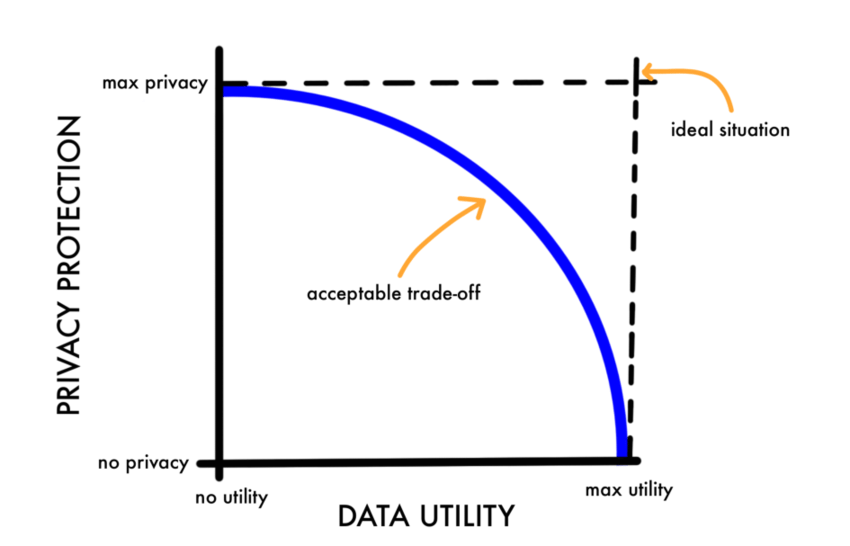
\includegraphics[width=0.75\textwidth]{images/privacy-filter/Data-Privacy-Protection-versus-Data-Utility.png}
    \caption{Illustration of the privacy-utility trade-off, from \citet{datasharing-implications}}
    \label{fig:privacy-utility-tradeoff}
\end{figure}

\noindent This chapter introduces the concept of \textit{privacy filters}, which dynamically strip away attributes of exposed data in accordance with some predefined rules. A prototype that implements privacy filters is developed for the \gls{CSS}\footnote{\url{https://github.com/CommunitySolidServer/CommunitySolidServer}} as a part of \middleware{}. The concrete implemenation of privacy filters as a software component was originally named \mwprivacy{} (short for Privacy-enhancing Plugin for Solid Applications). However, since it forms a part of the complete middleware, the specific implementation will hereafter also be referenced to as \middleware{}. This implementation provides a middleware in the Solid server which provides more fine-grained privacy control options. 

\begin{figure}[H]
\centering
\begin{subfigure}{.5\textwidth}
  \centering
  \begin{minted}[linenos,tabsize=2,breaklines]{json}
{
"accountOwner": "Jesse Geens",
"IBAN": "BE66123456783456",
"saldo": 665.53,
"currency": "EUR",
"history": [
    {
    "from": "BE17954824458821",
    "to": "BE66123456783456",
    "from_name": "Mark Jansen",
    "to_name": "Jesse Geens",
    "amount": 33.7,
    "timestamp": 1645447425,
    "description": "Payback borrowed money"
    }, {
    "from": "BE66123456783456",
    "to": "BE15954347627130",
    "from_name": "Jesse Geens",
    "to_name": "Steffie Smits",
    "amount": 10.0,
    "timestamp": 1645440365,
    "description": "Drinks"
    }
]}
  \end{minted}
  \caption{Data before applying privacy filter}
  \label{fig:data-before-privacy-filter}
\end{subfigure}%
\begin{subfigure}{.5\textwidth}
  \centering
  \begin{minted}[linenos,tabsize=2,breaklines]{json}
{
"accountOwner": "J.G.",
"IBAN": "BE42429824824354",
"saldo": 712.1171,
"currency": "EUR",
"history": [
    {
    "from": "BE17954824458821",
    "to": "BE42429824824354",
    "from_name": "Mark Jansen",
    "to_name": "J.G.",
    "amount": 34.8,
    "timestamp": 1645440000,
    "description": "Payback borrowed money"
    }, {
    "from": "BE42429824824354",
    "to": "BE15954347627130",
    "from_name": "J.G.",
    "to_name": "Steffie Smits",
    "amount": 9.45,
    "timestamp": 1645440000,
    "description": "Drinks"
    }
]}
  \end{minted}
  \caption{Data after applying privacy filter}
  \label{fig:data-after-privacy-filter}
\end{subfigure}
\caption{Example of data treatment by privacy filter, applied to financial transactions data}
\label{fig:example-treatment-privacy-filter}
\end{figure}

\newpage
\noindent In the developed prototype privacy filters are represented by a JSON document (per data scheme), describing which transformations ought to happen to which data attribute. An example of such a configuration file can be found in the appendix, in listing \ref{listing:privacy-filter-kbc}. Users can then specify how much privacy they want (in general, or for specific data types) in an abstract way using privacy levels, which are introduced in the next section. When a request is received, \middleware{} checks what data type it is, which application requested the data and what level of privacy the user has requested. Subsequently, a number of transformations are applied to the data (as specified by the configuration file), after which the transformed data is returned to the application. 

An example of what such a rewrite can look like is provided in figure \ref{fig:example-treatment-privacy-filter}. In this example, transformations such as \textit{pseudonym} (on the \texttt{accountOwner}, \texttt{name}, \texttt{IBAN} and \texttt{from}/\texttt{to} fields) and \textit{perturbation} (on the \texttt{saldo} and \texttt{amount} fields) are applied. A complete list of supported transformations is discussed in section \ref{sec:design-decisions}. The next section first discusses the earlier introduced concept of privacy levels, which provide granularity in the performed transformations. The subsequent sections then discuss how privacy filters were implemented as a part of \middleware{} by giving a detailed description of some important design decisions, followed by an overview of the architecture. Evaluation of the developed prototype is discussed in chapter \ref{cha:evaluation}.



\section{Privacy levels}
\label{sec:privacylevels}
\noindent In order to provide an intuitive mechanism for selecting which data is transformed, the concept of privacy levels is introduced. Privacy levels form an abstraction above the concrete data transformations and \gls{PETs} that are applied to the data before it is passed on to the application. This ensures that non-technical users can use a privacy-enhancing middleware, without needing to understand the technical details of the technologies and tactics that are employed. 

\middleware{} is configured with a default privacy level, but also supports specific privacy levels for certain data schemes. For example, a user could configure \middleware{} to use privacy level 2 by default, but privacy level 4 on bank transactions, since he does not want to expose this data. This makes the middleware more context-sensitive and allows for strong configurability. The privacy-utility trade-off can then also be taken into account for specific applications that need data with very high utility to deliver usable results. To make clear to the user what data is exposed an explanation should also be included (for every data type) which specifies concretely what will happen to the data under a certain privacy level.

Another important aspect is that the developers of privacy filters for specific data schemes must be aware of what privacy levels map to what leakage or tactics. This is best determined by privacy experts as it is a very complex topic. However, appendix \ref{appendix:privacy-levels} shows an example of such a mapping that was used to guide the development of configuration files for the prototype of \middleware{}.

\section{Architecture}
\label{sec:implementation}
\middleware{} is implemented as an extension of the \acrlong{CSS}. The complete code and instructions can be found at \url{https://github.com/jessegeens/pepsa-component}. First, a number of important design decisions are discussed in this section. Afterwards, the concrete implementation of privacy filters as an extension of the \gls{CSS} is reviewed.

\subsection{Design decisions}
\label{sec:design-decisions}
In every architectural design, important decisions have to be made based on some sort of cost-benefit analysis: there is no free lunch. Similarly, this is the case with the design of \middleware{}. This section describes the reasoning behind a number of important design decisions that have been made during the modelling and development.

\subsubsection{Positioning}
A first important aspect of the design of \middleware{} is where it is logically positioned. The choice was made to position the middleware as an extension of an existing Solid server (in our case, the \gls{CSS}). In this regard it is a true middleware. Furthermore, this results in significantly sped up development, as well as much better performance. A disadvantage of this approach is that it leads to more centralization: if a user is using a pod provided by a third-party not running \middleware{}, there is no way to enable this. Extending an existing solid server also means choosing one specific server to support, making the solution incompatible with other servers. However, developing the middleware as an extension of a Solid server makes it such that it does not really interact with the Solid protocol itself. As such, the middleware becomes much easier to keep up-to-date with the quickly evolving Solid specification. 
%Lastly, developing \middleware{} as an extension of a Solid server also enables it to form a complete middleware when combined with the new access token mechanism.

The other possibility that was considered would be to build \middleware{} as a proxy. Requests from the Solid application would be directed to \middleware{} instead, which fetches the data, sanitizes it, and then replies with the sanitized data. This is a much less centralized option, but comes at a big performance cost. There are is more network usage and double the number of HTTP requests, for example. However, there is also a very important technical limitation. As was discussed in section \ref{sec:solid-oidc}, Solid uses \gls{DPoP} tokens. As can be seen in listing \ref{listing:dpop}, the \texttt{htu} parameter of the \gls{DPoP} token body prevents this token from being used in another pod, essentially making the proxy solution impractical when communicating with a Solid server using this authentication mechanism.


\subsubsection{Supporting multiple data schemes}
Solid supports storing nearly any type of resource, both linked and non-linked. The data that is most prone to leakage in the context of a data aggregator is structured data. Structured data can take many forms, and any good middleware should be independent of the types of structured data that are requested or passing through it. However, \middleware{} needs to perform operations on the data that passes through it, and should thus have some context as to how it should handle a specific data scheme.

This is realized by providing \middleware{} with an internal library of parsers for each content representation, which support a predefined set of transformations. For example, there is a component that performs pseudonymization on data that is represented in JSON. At startup, the software reads a number of configuration files, one for every supported data scheme. These files then specify how a data scheme should be detected, and what transformations ought to be applied to it. Some disadvantages of this approach are that this requires more up-front coding to support this library of transformations for content representations. There is also a computational cost associated with having to parse all these configuration files and apply the rules expressed in them, instead of directly executing code. Despite these drawbacks, there is also a very large advantage to this approach: supporting new data schemes becomes a much easier and faster task. The only work that needs to be performed to support a new data scheme would be to write a scheme configuration file, something that can be done in a few hundred lines of JSON. The appendix contains the JSON Schema used to describe such configuration files (see listing \ref{listing:privacy-filter-jsonschema}) as well as an example of such a scheme configuration file (see listing \ref{listing:privacy-filter-kbc}). This configuration file is aimed specifically at use case \ref{usecase:personal-finance}.

\noindent Another possibility that was considered would be to have separate components, where each component is responsible for performing transformations on the input data of a specific data scheme. The components would be loaded dynamically at run-time, using dependency injection technology such as \textit{components.js}\footnote{\url{https://componentsjs.readthedocs.io/en/latest/}}. This would result in great flexibility: the transformation component can perform virtually any transformation. However, a first big disadvantage of this strategy is that it results in a significant development time for each component (and thus, for every supported data scheme). This can result in a lack of support for many (popular) data schemes, making \middleware{} significantly less useful. Another major downside is that this imposes new weaknesses from a security point-of-view, as untrusted code is imported in and executed on the Solid server. The main reason for not using this technique is that the cost of writing new components specifically for one data scheme is too high for the relatively meager advantages it gives over the other approach. 


\begin{table}[H]
\begin{center}
\begin{tabulary}{\textwidth}{p{0.20\textwidth}p{0.8\textwidth}}
\textbf{Transformation name} & \textbf{Description}                                                                                                                                                          \\ \hline
Remove               & The targeted and deliberate omission of PII from the data record or data set.                                                                                                 \\
Pseudonym            & The systematic replacement of direct identifiers with surrogates, whereby the mapping between surrogate and identity is kept separately.                                      \\
Perturbation         & The insertion of randomized noise into the values of the data to hide exact values                                                                                 \\
Random               & Tactics that involve the modification of PII attribute values/records by injecting artificial random elements.                                                                \\
Encrypt              & Using cryptographic means to encode the PII attribute values / records / datasets.                                                                                            \\
Hash                 & Using cryptographic hash functions to obfuscate the PII attribute values / records / datasets in a deterministic fashion.                                                                                            \\
\end{tabulary}
\caption{Overview of data transformations supported in \middleware{}}
\label{table:supported-transformations}
\end{center}
\end{table}

\subsubsection{Supported transformations}
Table \ref{table:supported-transformations} gives an overview of which transformations are currently supported. The choice for supported transformations is mostly based on the discussion from section \ref{sec:transformation-approaches}, which described a taxonomy of architectural tactics involving data transformations. Some tactics could, however, not be mapped to an equivalent tactic in our middleware. An example of this is the \textit{Aggregate} tactic as \middleware{} does not support grouping data elements, since data is treated on a per-attribute basis. Similar arguments hold for other tactics that are not supported. The \textit{Perturbation} tactic is based on the \textit{Blur} tactic from table \ref{table:de-id-taxonomy}, but renamed to convey its applicability to numeric values. Similarly, \textit{Encrypt} is supported along with the similar \textit{Hash} tactic.

\subsection{Implementation in CSS}
The implementation of \middleware{} is realised as an extension of the \acrlong{CSS}, leveraging components.js to substitute a component of the \gls{CSS} with a component provided by \middleware{}. An overview of the architecture of the \gls{CSS} is presented in figure \ref{fig:solid-arch}.

Concretely, the main component of \middleware{} is the \texttt{AnonymizingHTTPHandler}, which extends the \texttt{OperationHttpHandler} class provided by the \gls{CSS}. Using a custom components.js configuration, this new class is injected into the \gls{CSS} by giving it as an argument to the \texttt{ParsingHttpHandler}. On diagram \ref{fig:solid-arch} in the appendix, this is located under \texttt{AuthenticatedLdpHandler}. A configuration file for the \gls{CSS} specifying the dependency injection of the \texttt{AnonymizingHTTPHandler} can also be found in the appendix, under listing \ref{listing:css-config}.

Figure \ref{fig:arch-overview} gives an overview of the system architecture of \middleware{}. Components that are part of a vanilla version of the \gls{CSS} are colored in blue. The red component, \texttt{AnonymizingHTTPHandler}, is the main component of the middleware and is the component that is injected into the \gls{CSS}. The parsers (in yellow) are also included dynamically through the configuration file (listing \ref{listing:css-config}), such that other content representations can also easily be supported. The \texttt{ParserSelector} can then, based on the content representation that is defined in the detected data scheme, select the correct parser to perform the execution of all specified transformations. 
Figure \ref{fig:pepsa-sequence} illustrates the flow of how a privacy filter is applied to an incoming request in the \gls{CSS}.

\begin{sidewaysfigure}[h]
    \centering
    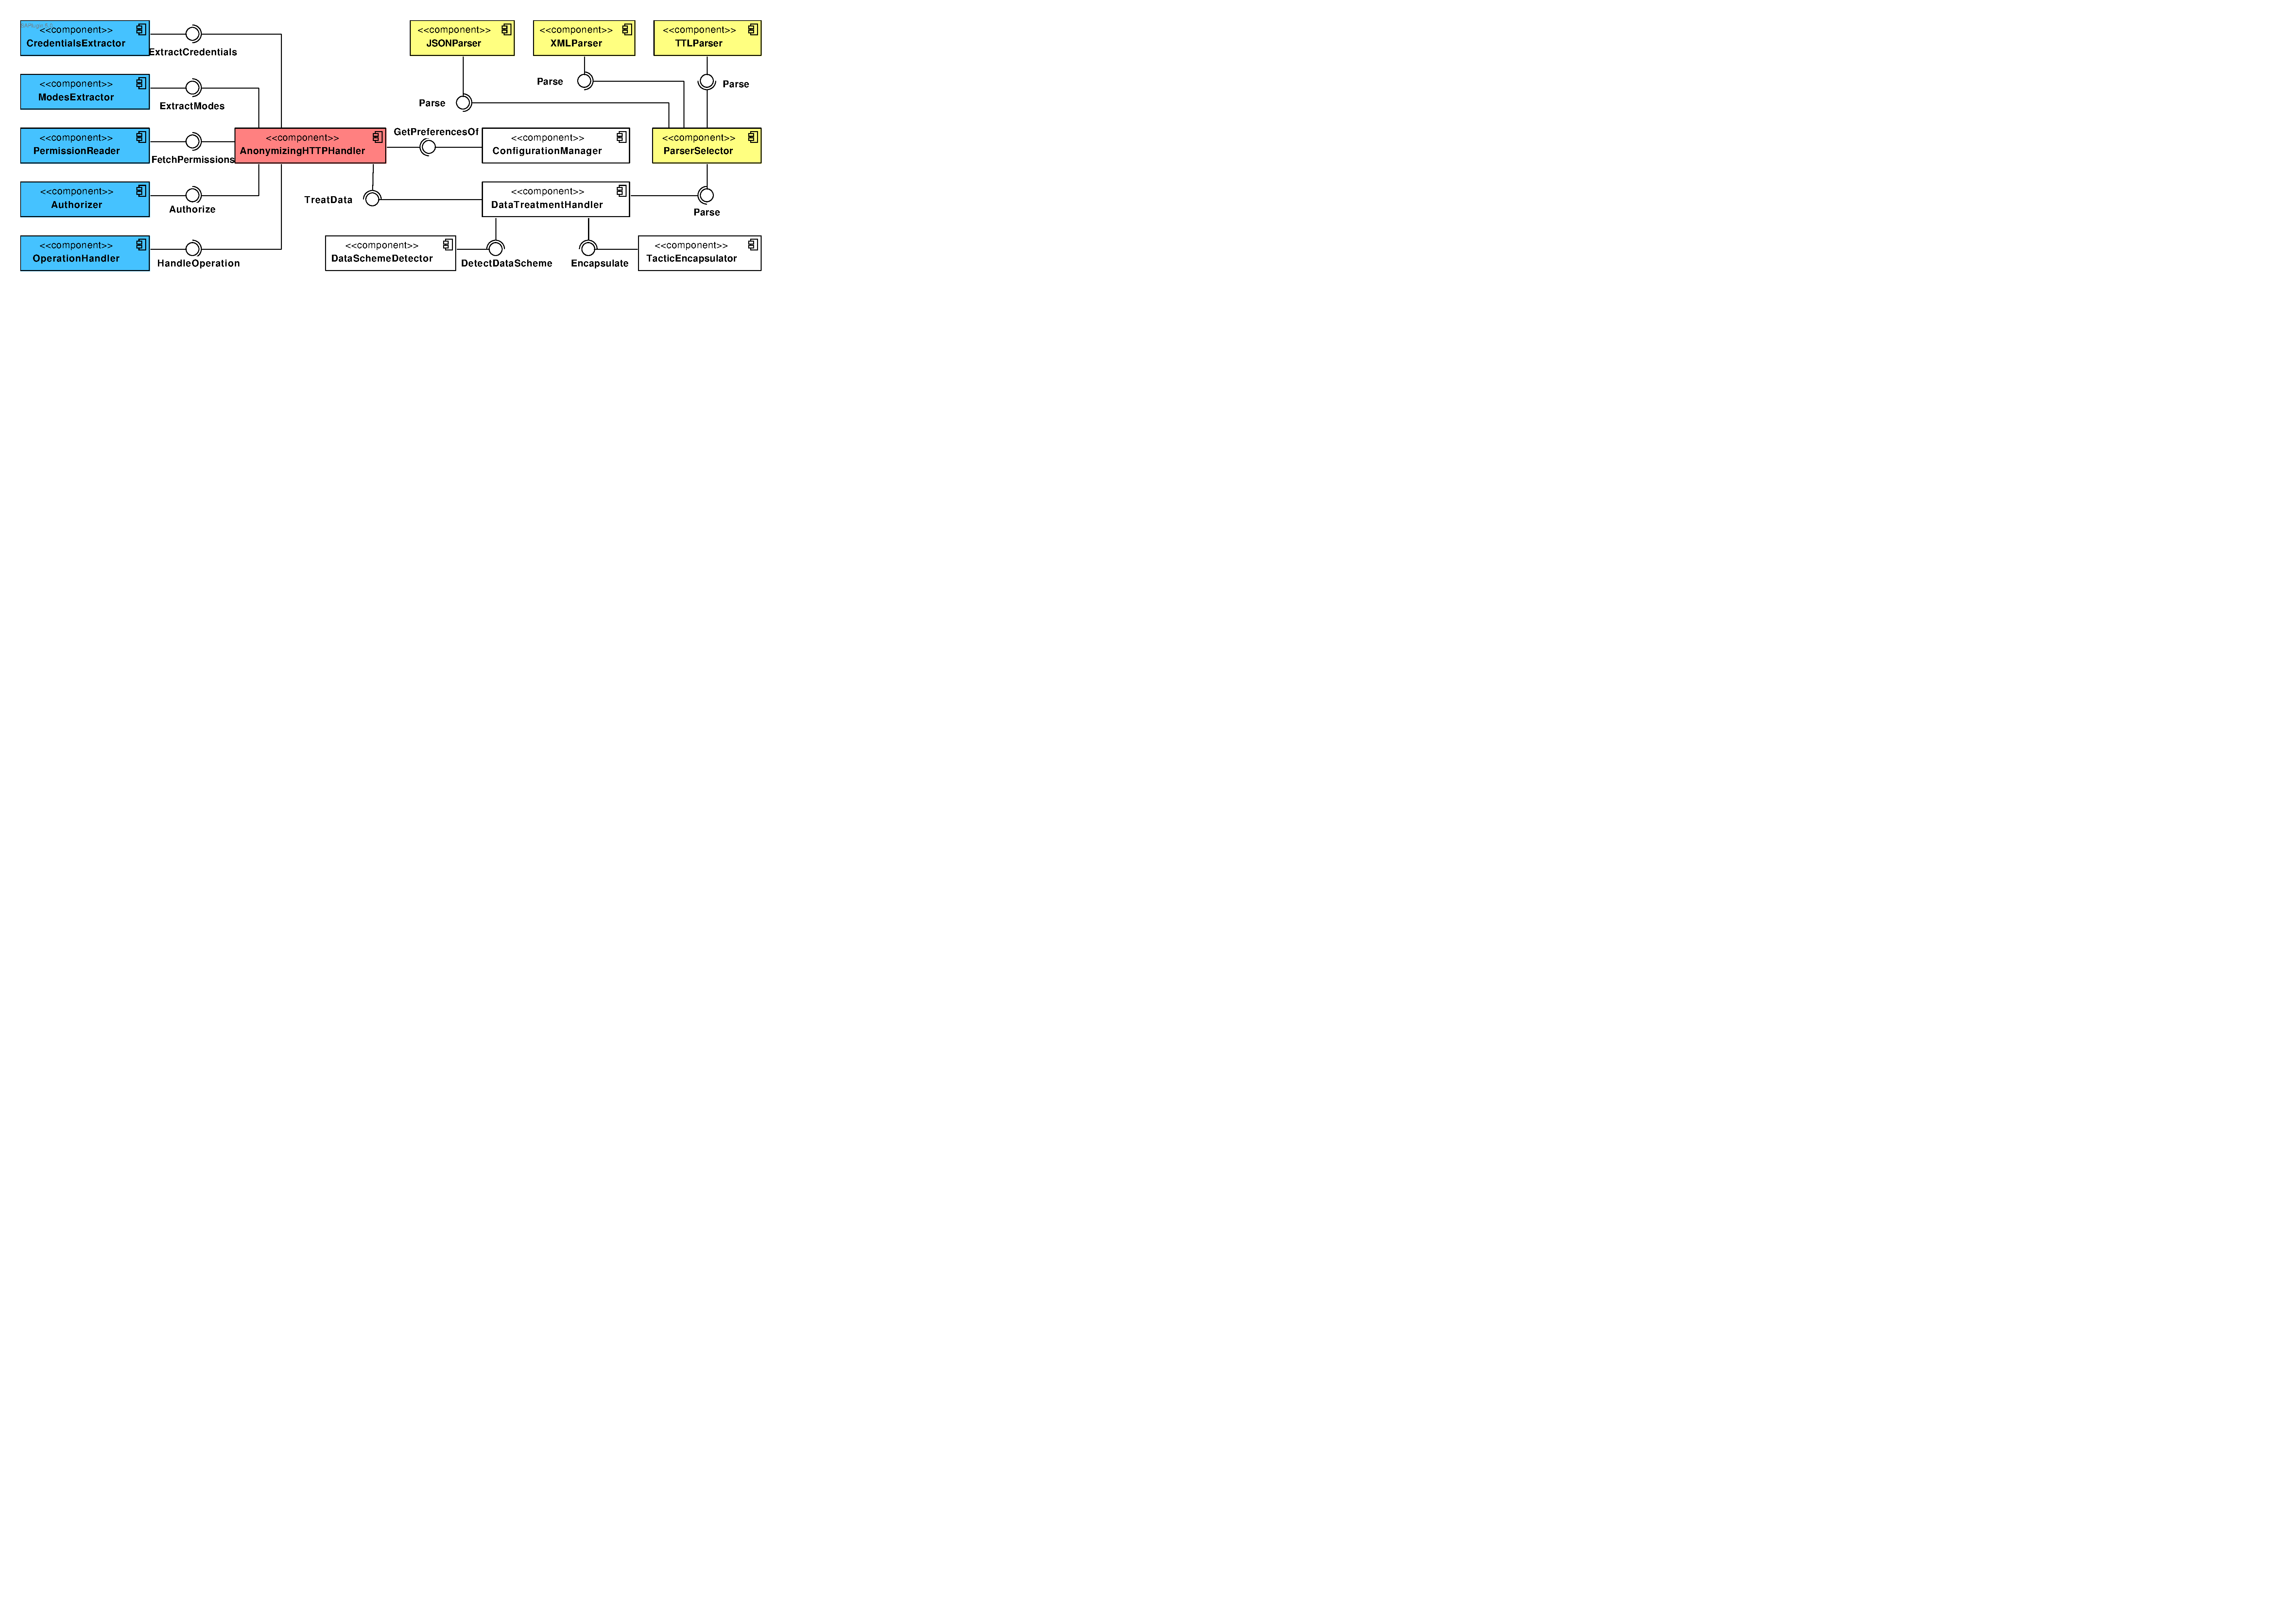
\includegraphics[width=1.0\textwidth]{images/architecture/PePSA-System-Overview.pdf}
    \caption{Overview of \middleware{} privacy filter architecture}
    \label{fig:arch-overview}
\end{sidewaysfigure}



\begin{sidewaysfigure}[h]
    \centering
    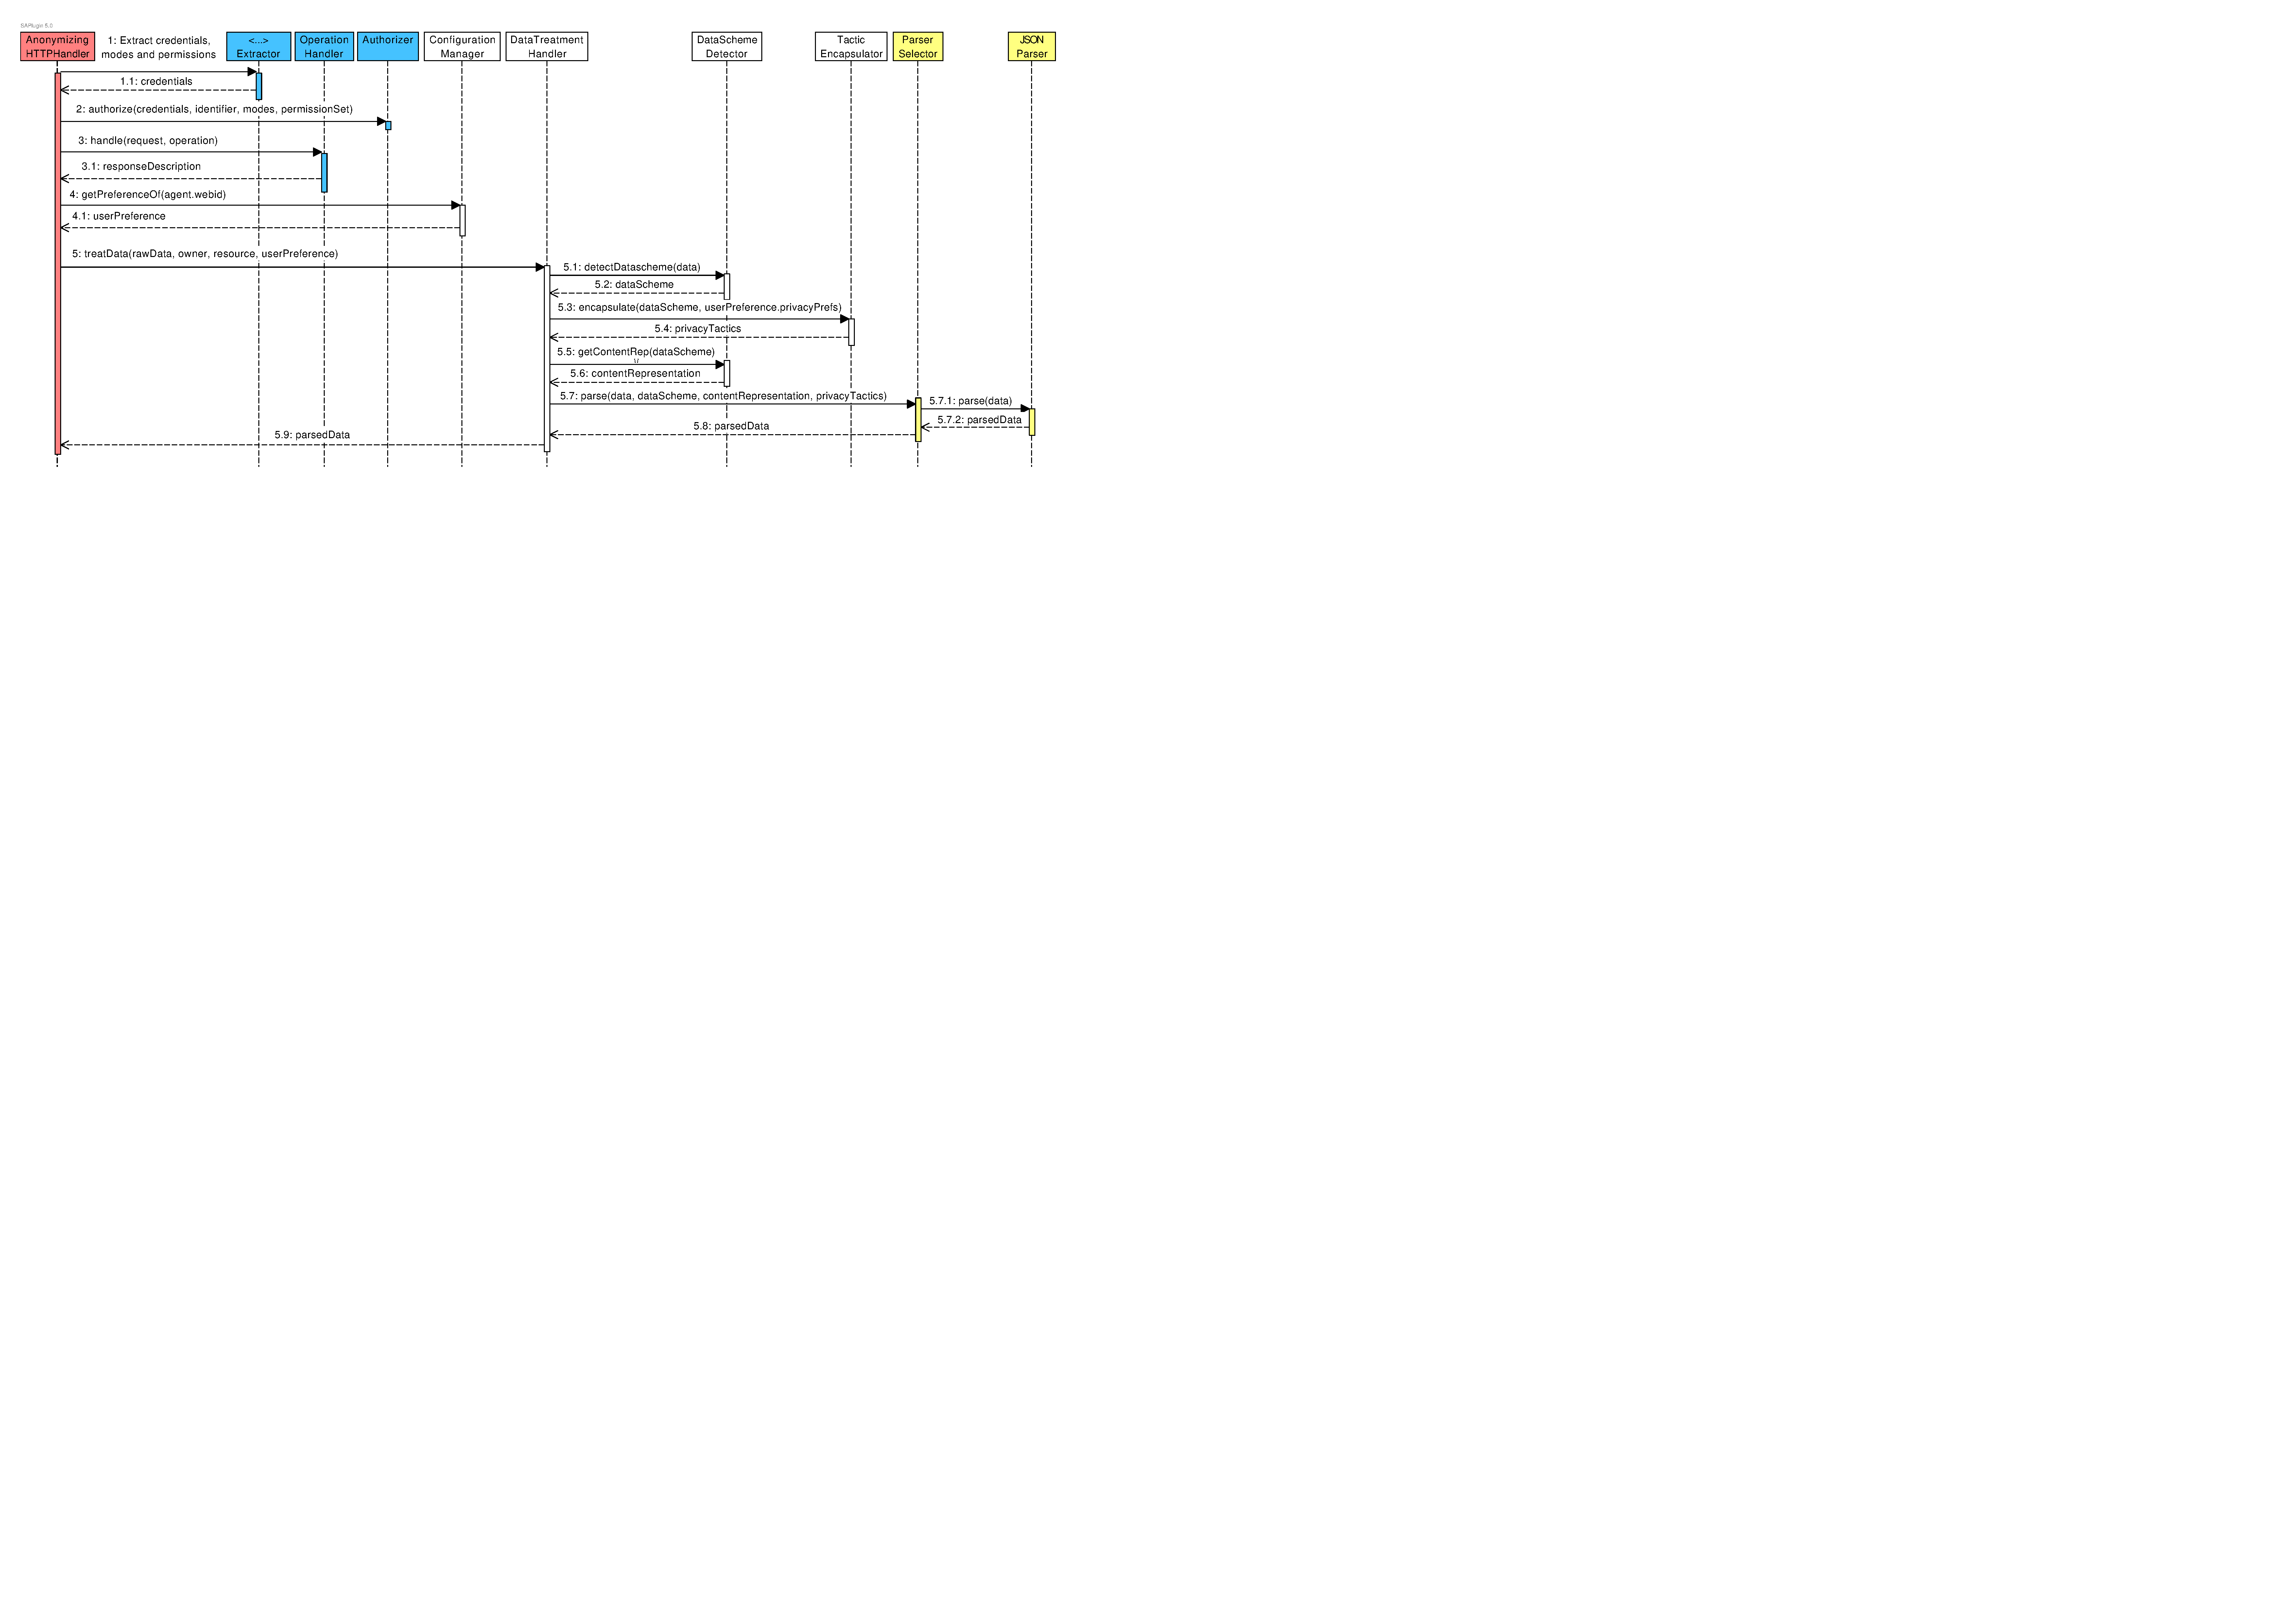
\includegraphics[width=1.0\textwidth]{images/architecture/InteractionDiagram-Rewrite-Flow-PePSA.pdf}
    \caption{Flow of \middleware{} request rewrite}
    \label{fig:pepsa-sequence}
\end{sidewaysfigure}
\chapter{Macaroons as a novel access token mechanism in Solid}
\label{cha:macaroons-solid}

Section \ref{sec:macaroons} gave an introduction to macaroons, a novel kind of access tokens. This chapter discusses ways in which macaroons can mediate the problems stipulated in chapter \ref{cha:solution-overview}. The first part of this chapter focuses on group vaults, or pods that are controlled by multiple users. The second part of the chapter focuses on how macaroons can enable decentralized access token delegation, by highlighting how token delegation works traditionally and illustrating the improvements macaroons bring here.

One of the problems that was identified in section \ref{sec:generic-agg-arch} was the high computational cost of a token mechanism that uses public-key cryptography. A lower computational cost is realized by macaroons because of its hash-based signatures, instead of using public-key cryptography. Real performance gains of utilising macaroons instead of \gls{DPoP} are explored in section \ref{sec:macaroons-performance}. Using macaroons for realizing group vaults and decentralized delegation is explored in the next sections. 

\section{Group vaults}
\label{sec:group-vaults}
Group vaults are pods which hold data of multiple users in a single pod. This could be useful in many scenarios, for example a pod which holds data for a family (such as incoming invoices, controlling light switches in the home, etc.). However, realizing secure group vaults poses problems due to the decentralized nature of Solid. Users in a group vault can have identities that are issued by different services. For example, users \textit{Alice}, with WebID \texttt{https://alice.solid.org} (issued by \texttt{solid.org}), and \textit{Bob}, with WebID \texttt{https://bob.pods.org} (issued by \texttt{pods.org}), would like to open a group vault. When a request is made to the group server (for modifying or reading a resource), a token must be included that authenticates Alice or Bob. However, the group vault server is not the server that issued the token. Moreover, the token server that must be contacted for validating the user's identity is dependent on which user makes the request. When the traditional authentication mechanism of Solid is used, this can cause a bottleneck on the token server. 

Macaroons can bring a solution to this problem due to one of its features called \textit{third-party attestation}. In this mechanism, a macaroon can contain a caveat (requirement) that must be attested by a third party. This third party can then generate a \textit{discharge macaroon}, which serves as a proof that the caveat laid out in the original macaroon is fulfilled. In the case of group vaults, these third-party attestations can be used to prove to the group vault server that a user is authenticated by a third-party identity provider. This section explores an architecture for a group vault server which uses macaroons to authenticate its participants.

\subsection{Group vault architecture}
Group vaults are Solid pods that store data for a group of participants. Traditionally, such as for example in the \acrlong{CSS}, the server that hosts the pod (the data) is the same server that acts as the token endpoint for verifying access tokens of the user. In the context of group vaults, the \gls{GVS} does not issue tokens and as such can not verify them. Instead, the \gls{GVS} keeps track of which users belong to the group and holds the data belonging to the group vault.

When a user wishes to access a group resource, it fetches a macaroon from the \gls{GVS}, specifying his WebID and the group from which he would like to access resources. The \gls{GVS} then issues a macaroon, limiting its use to that specific user, and including a caveat that the user is logged in at his identity provider. The user must then contact his own token endpoint and request a discharge macaroon, which serves as proof of his authentication. The user can then request resources from the \gls{GVS} by including his macaroon and its associated discharge macaroon. If many successive requests must be made (for example, fetching the contents of a resource container), the token endpoint of the user must only be contacted once and the discharge macaroon (or one derived from this) can be re-used multiple times. 

Figure \ref{fig:gv-macaroon-flow} illustrates the flow of a user requesting a resource from a \gls{GVS}. The \gls{GVS} guarantees that only the correct server can create the discharge macaroon, by encrypting the necessary caveat key with the token endpoint's public key. The location of this public key can be found in the \texttt{openid-configuration} file. An example lay-out of the macaroon caveats can be seen in figure \ref{fig:gv-macaroon-example}.
%Figure \ref{fig:gv-sys-overview} illustrates the system overview of a group vault architecture. 

To verify the feasibility of using macaroons as access tokens for realizing efficient group vaults, a prototype has been developed in JavaScript, leveraging the macaroons.js library\footnote{See \url{https://www.npmjs.com/package/macaroons.js/v/0.1.0}}. The prototype is not built following the Solid specification but implements all the necessary features for validating the general architecture. The source code of this prototype can be found at \url{https://github.com/jessegeens/groupvault-demo}.

%\begin{figure}[h]
%    \centering
%    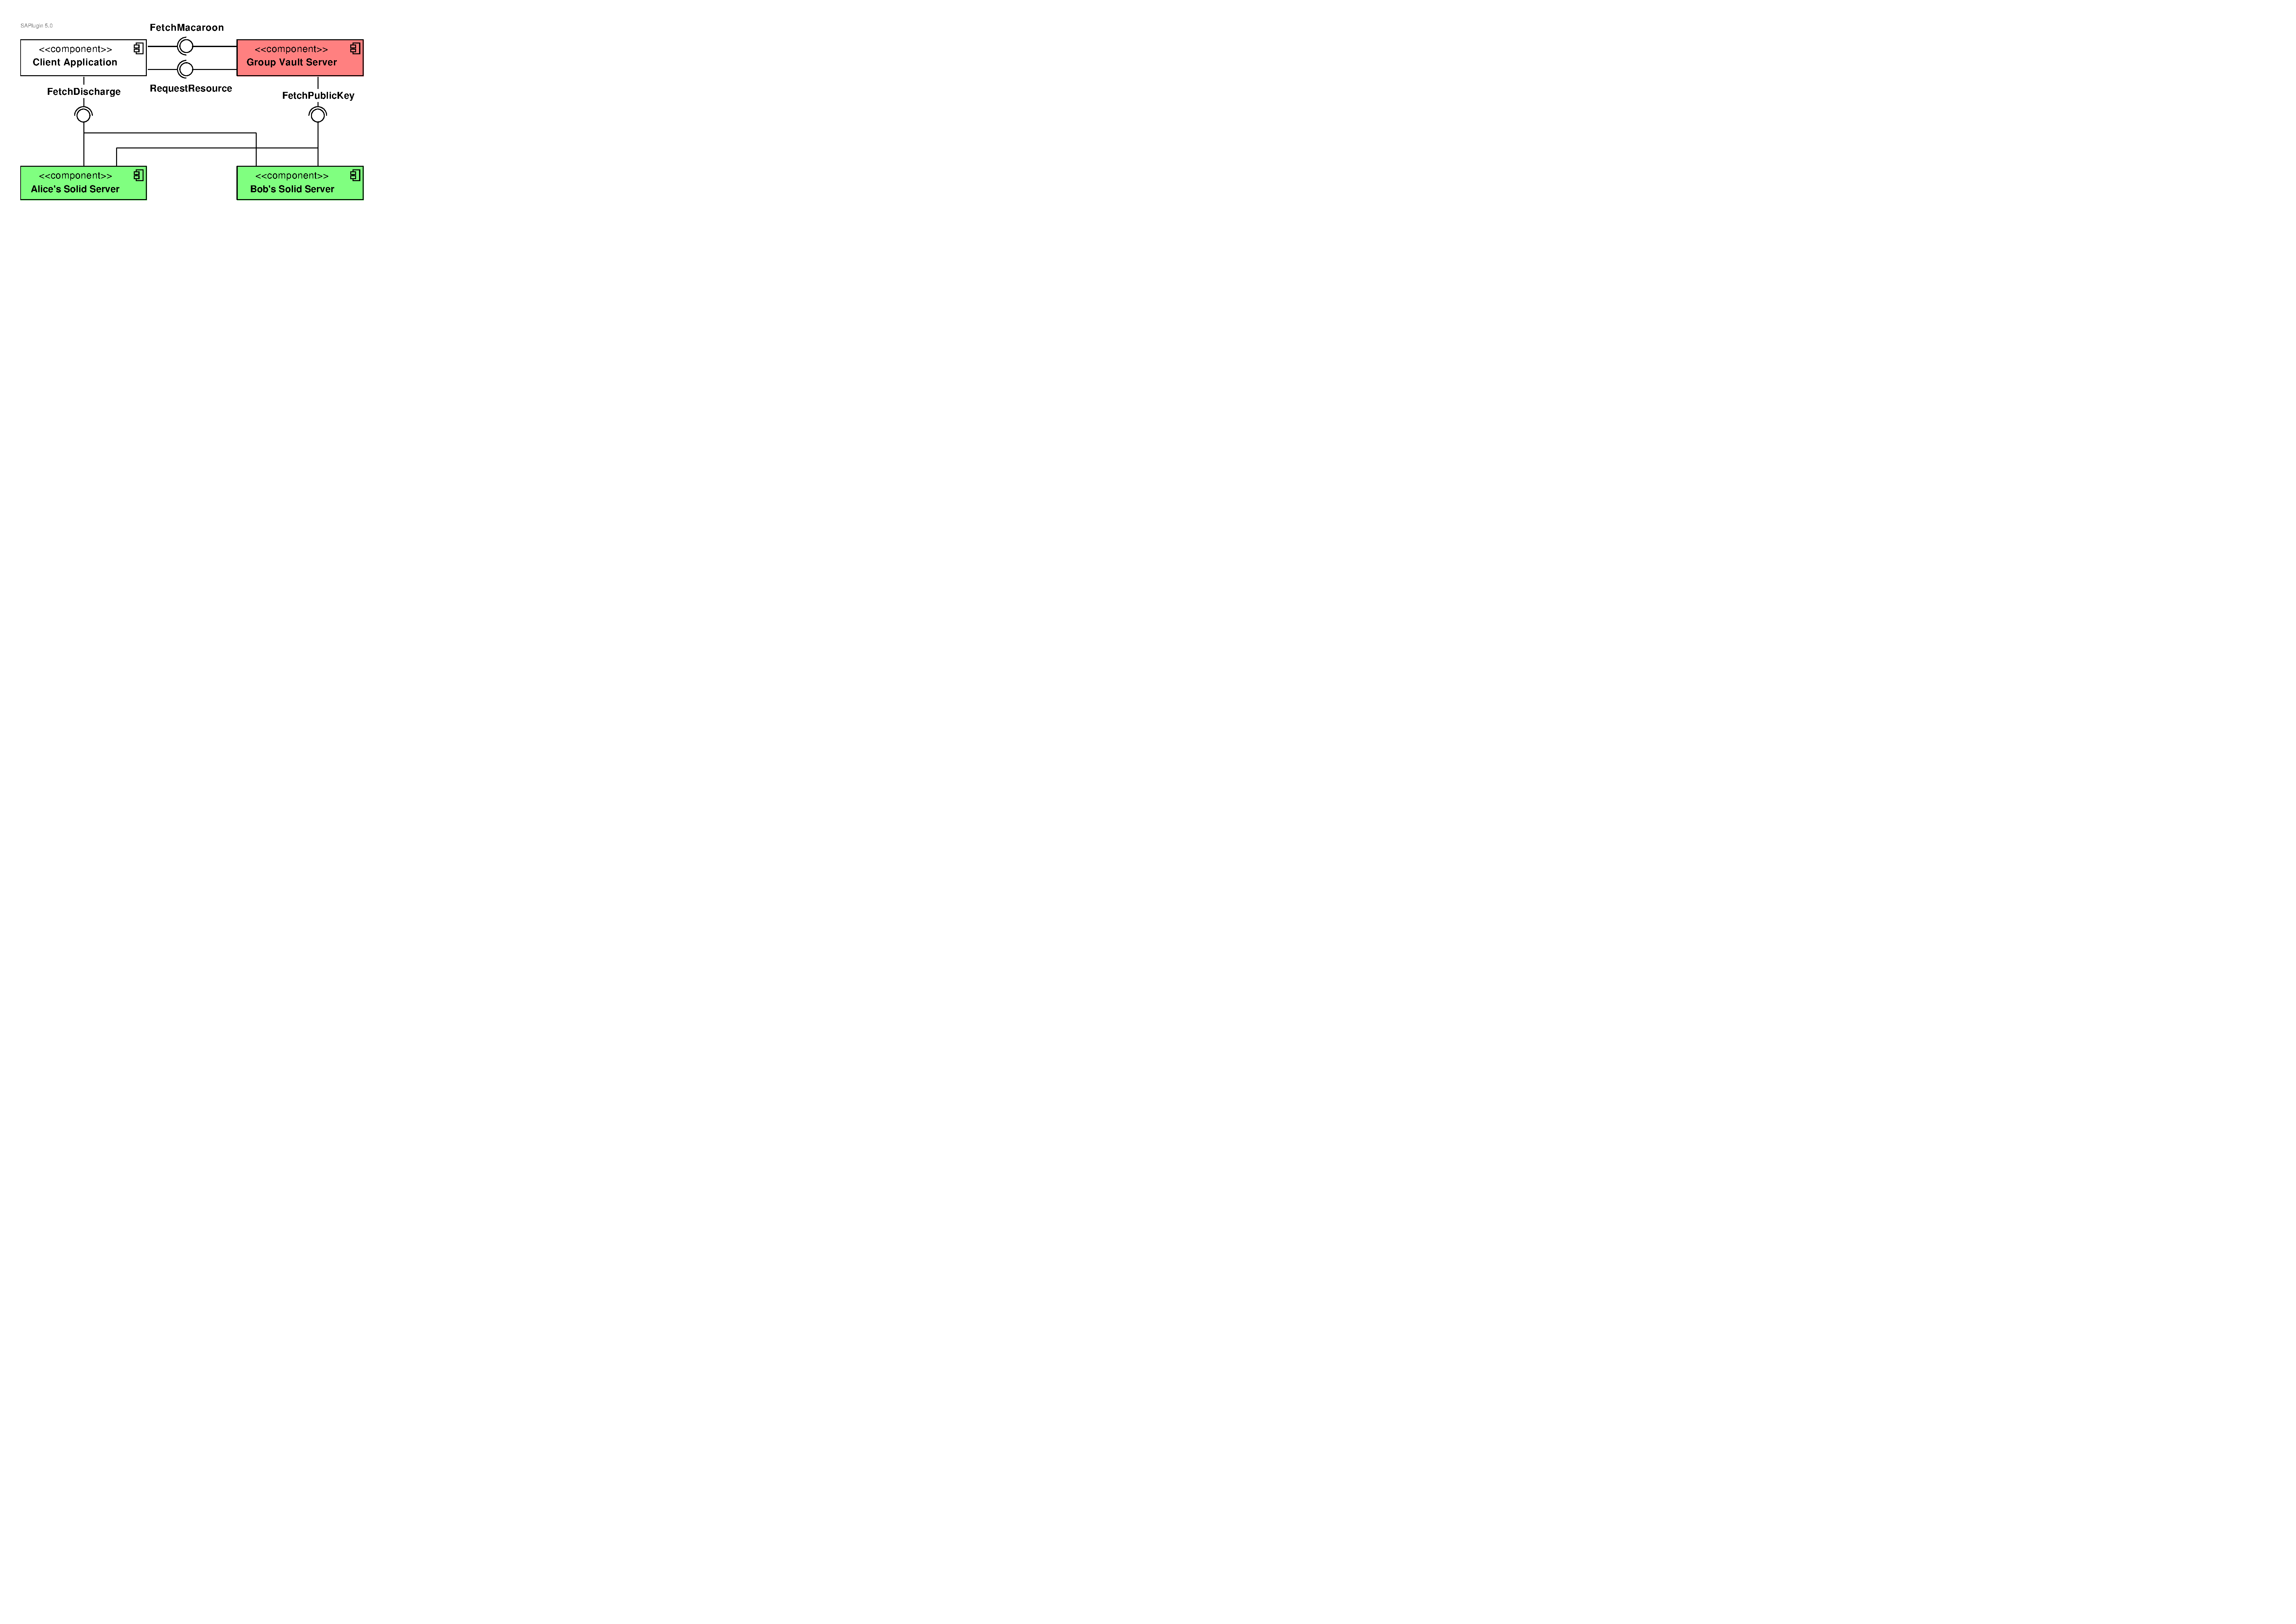
\includegraphics[width=0.45\textwidth]{images/macaroons-solid/ComponentDiagram-Group-Vault-System-Overview.pdf}
%    \caption{System Overview of a Group Vault architecture.}
%    \label{fig:gv-sys-overview}
%\end{figure}

\begin{figure}[h]
    \centering
    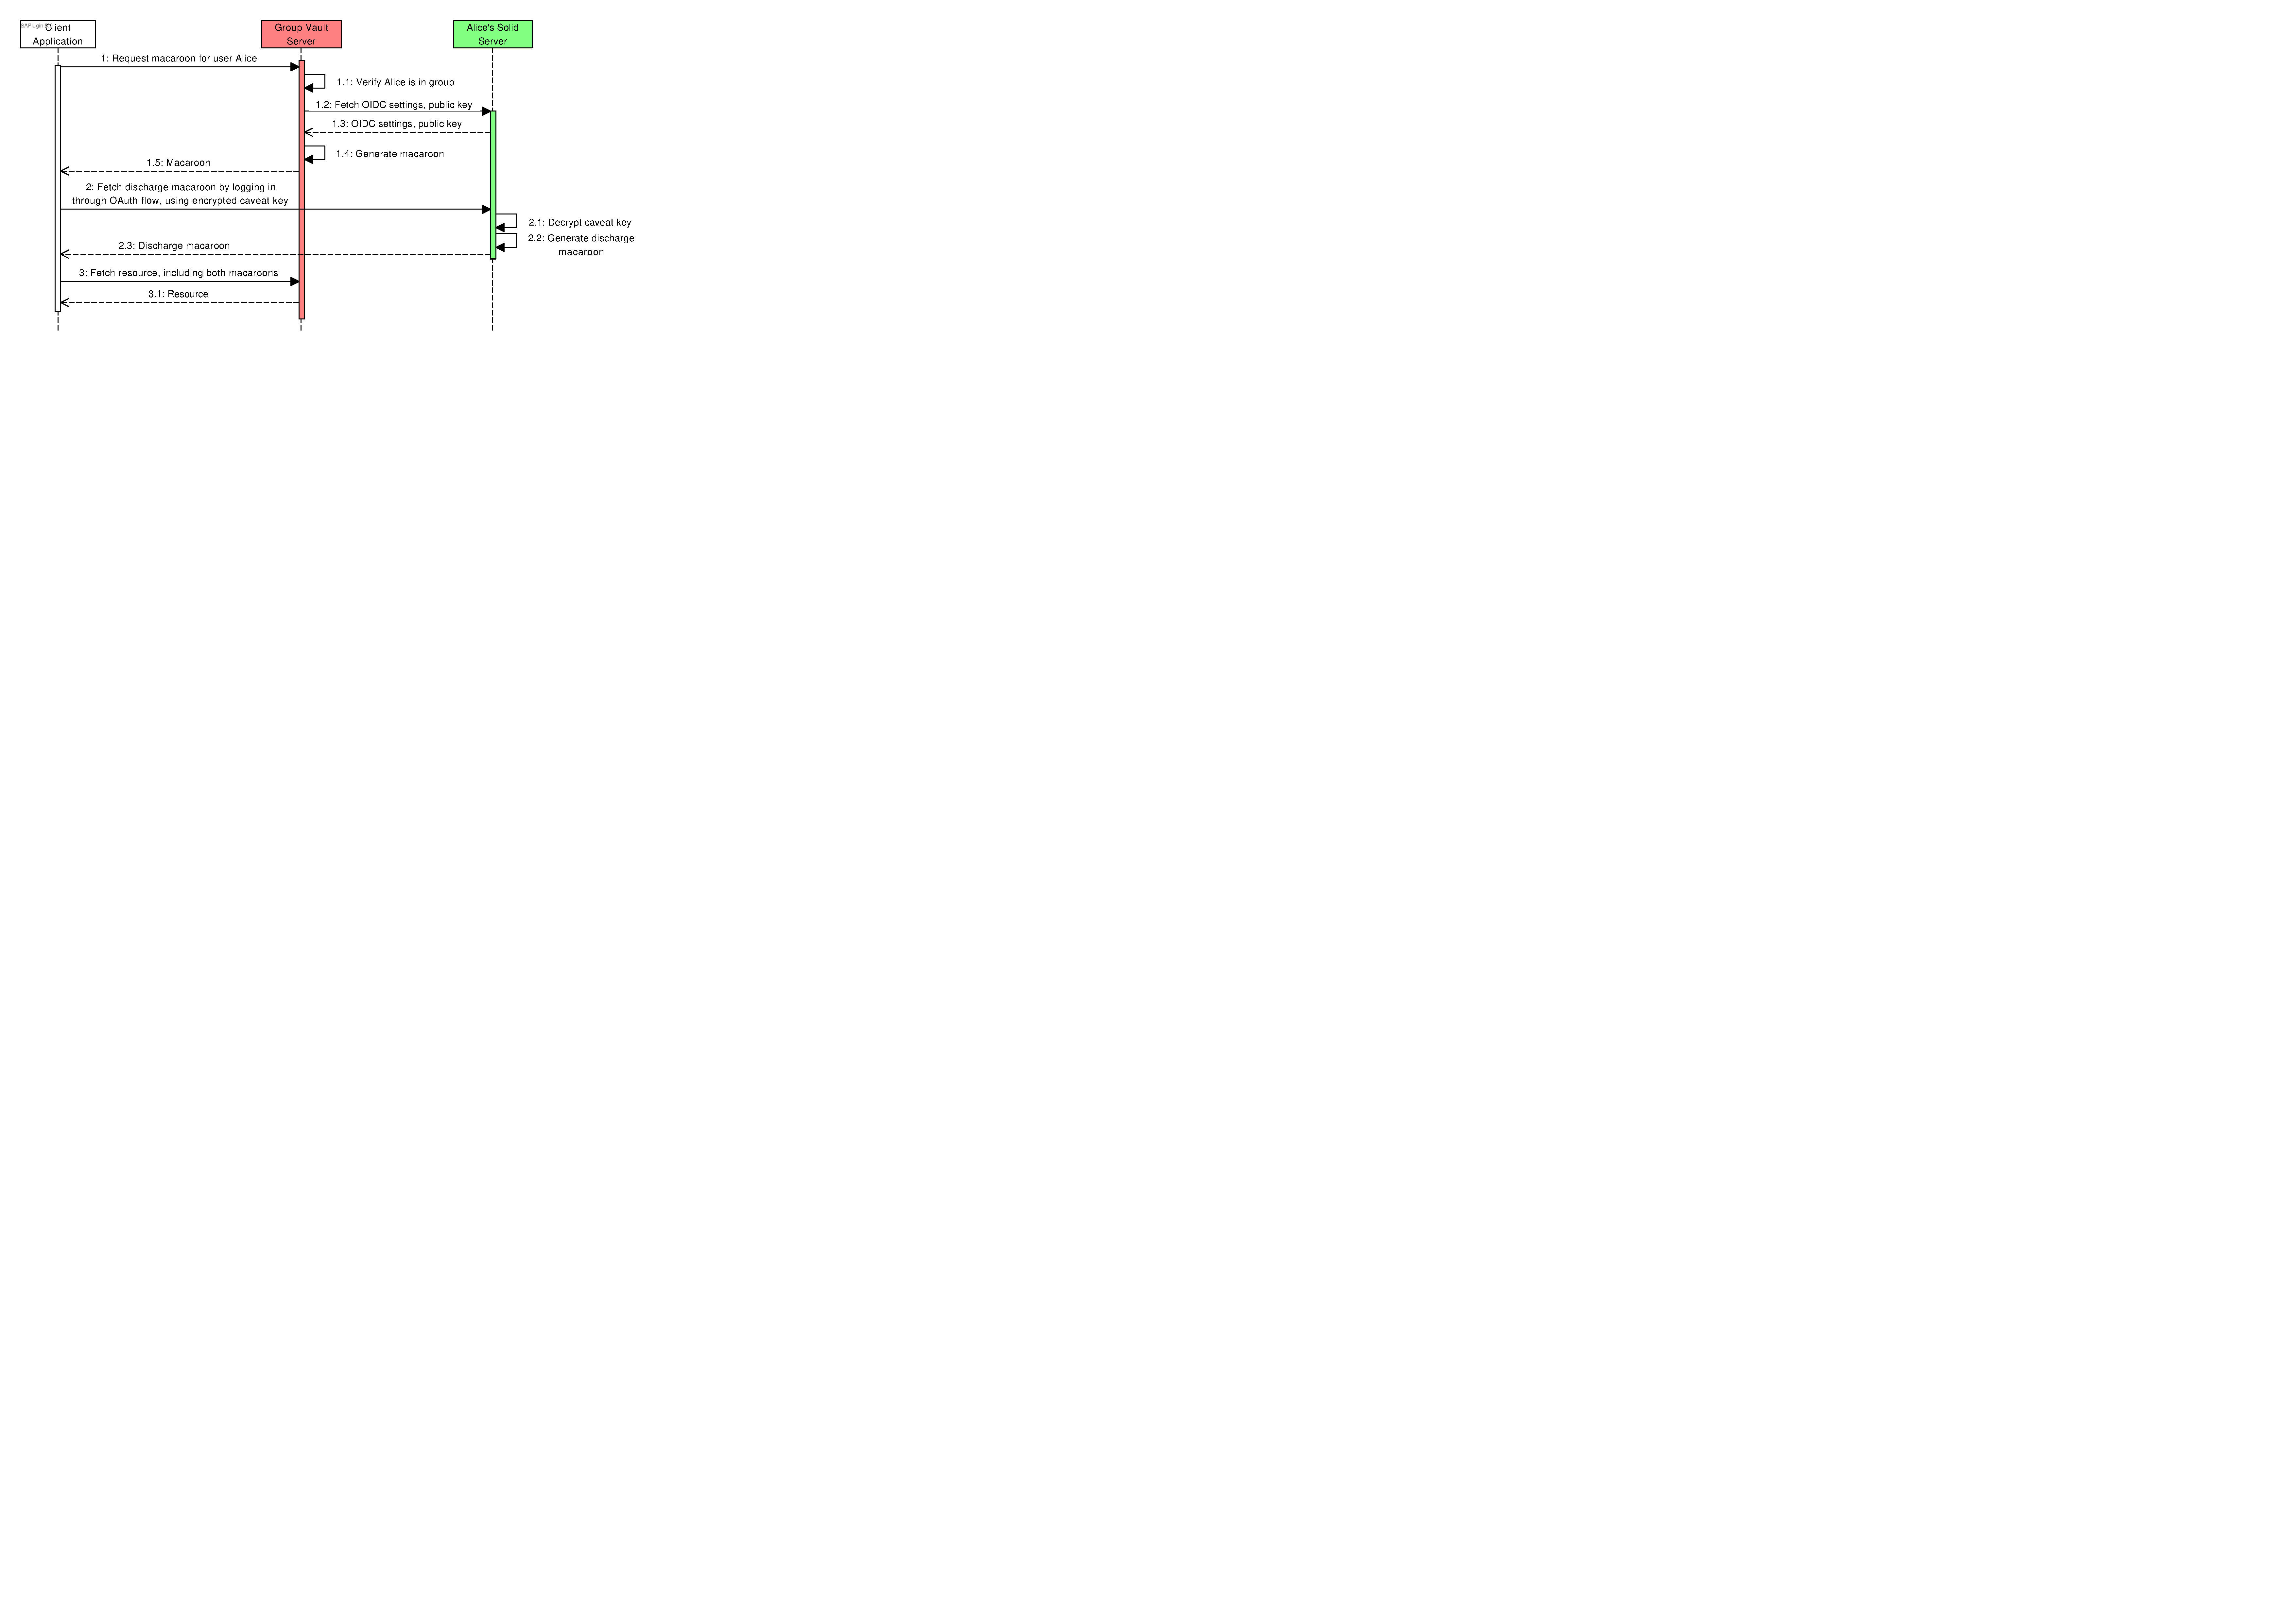
\includegraphics[width=1.0\textwidth]{images/macaroons-solid/InteractionDiagram-Group-Vault-Authentication-Flow.pdf}
    \caption{Authentication flow for accessing a resource from a \acrlong{GVS}.}
    \label{fig:gv-macaroon-flow}
\end{figure}

\begin{figure}[H]
    \centering
    {\fontfamily{qag}\selectfont }

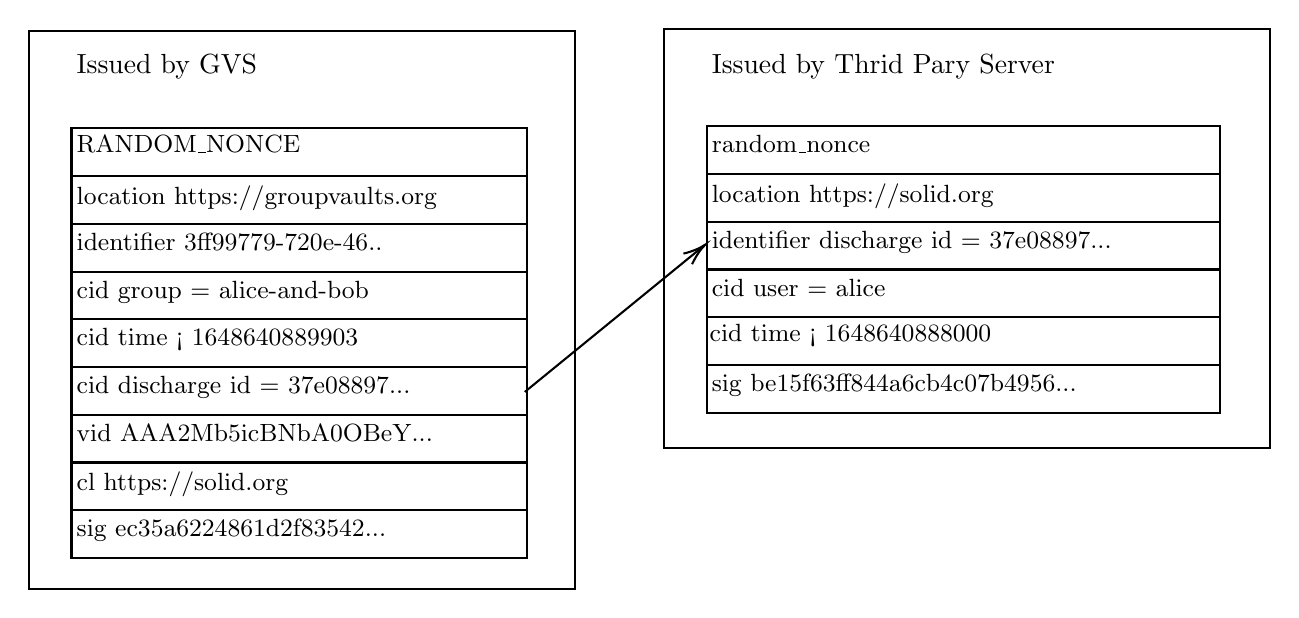
\begin{tikzpicture}[x=0.75pt,y=0.75pt,yscale=-1,xscale=1]
%uncomment if require: \path (0,331); %set diagram left start at 0, and has height of 331

%Shape: Rectangle [id:dp36106898781320174] 
\draw   (25,35) -- (288,35) -- (288,304) -- (25,304) -- cycle ;
%Shape: Rectangle [id:dp014069378908031283] 
\draw   (45.6,82) -- (265,82) -- (265,105) -- (45.6,105) -- cycle ;
%Shape: Rectangle [id:dp20345726322429547] 
\draw   (45.6,151) -- (265,151) -- (265,174) -- (45.6,174) -- cycle ;
%Shape: Rectangle [id:dp7088154428740524] 
\draw   (45.6,105) -- (265,105) -- (265,128) -- (45.6,128) -- cycle ;
%Shape: Rectangle [id:dp7951647364061636] 
\draw   (45.6,243) -- (265,243) -- (265,266) -- (45.6,266) -- cycle ;
%Shape: Rectangle [id:dp2294119235309251] 
\draw   (45.6,128) -- (265,128) -- (265,151) -- (45.6,151) -- cycle ;
%Shape: Rectangle [id:dp20892929793325288] 
\draw   (45.6,174) -- (265,174) -- (265,197) -- (45.6,197) -- cycle ;
%Shape: Rectangle [id:dp675591301361505] 
\draw   (45.6,266) -- (265,266) -- (265,289) -- (45.6,289) -- cycle ;
%Shape: Rectangle [id:dp946669631946771] 
\draw   (45.6,220) -- (265,220) -- (265,243) -- (45.6,243) -- cycle ;
%Shape: Rectangle [id:dp8118838011942326] 
\draw   (45.6,197) -- (265,197) -- (265,220) -- (45.6,220) -- cycle ;
%Shape: Rectangle [id:dp1748336079202455] 
\draw   (331,34) -- (623,34) -- (623,236) -- (331,236) -- cycle ;
%Shape: Rectangle [id:dp6959528817165129] 
\draw   (351.6,81) -- (599.08,81) -- (599.08,104) -- (351.6,104) -- cycle ;
%Shape: Rectangle [id:dp9148042784412247] 
\draw   (351.6,150) -- (599.08,150) -- (599.08,173) -- (351.6,173) -- cycle ;
%Shape: Rectangle [id:dp2637371441526388] 
\draw   (351.6,104) -- (599.08,104) -- (599.08,127) -- (351.6,127) -- cycle ;
%Shape: Rectangle [id:dp8589922967246587] 
\draw   (351.6,127) -- (599.08,127) -- (599.08,150) -- (351.6,150) -- cycle ;
%Shape: Rectangle [id:dp12106124639103755] 
\draw   (351.6,173) -- (599.08,173) -- (599.08,196) -- (351.6,196) -- cycle ;
%Shape: Rectangle [id:dp8847449056516175] 
\draw   (351.6,196) -- (599.08,196) -- (599.08,219) -- (351.6,219) -- cycle ;
%Straight Lines [id:da2707605121887615] 
\draw    (264,209) -- (349.45,139.26) ;
\draw [shift={(351,138)}, rotate = 140.78] [color={rgb, 255:red, 0; green, 0; blue, 0 }  ][line width=0.75]    (10.93,-3.29) .. controls (6.95,-1.4) and (3.31,-0.3) .. (0,0) .. controls (3.31,0.3) and (6.95,1.4) .. (10.93,3.29)   ;

% Text Node
\draw (46.6,45) node [anchor=north west][inner sep=0.75pt]   [align=left] {Issued by \acrlong{GVS}};
% Text Node
\draw (46.6,84) node [anchor=north west][inner sep=0.75pt]   [align=left] {{\small RANDOM\_NONCE}};
% Text Node
\draw (46.6,108) node [anchor=north west][inner sep=0.75pt]   [align=left] {{\small location https://groupvaults.org}};
% Text Node
\draw (46.6,131) node [anchor=north west][inner sep=0.75pt]  [font=\small] [align=left] {identifier 3ff99779-720e-46..};
% Text Node
\draw (46.6,154) node [anchor=north west][inner sep=0.75pt]  [font=\small] [align=left] {cid group = alice-and-bob};
% Text Node
\draw (46.6,177) node [anchor=north west][inner sep=0.75pt]  [font=\small] [align=left] {cid time < 1648640889903};
% Text Node
\draw (46.6,200) node [anchor=north west][inner sep=0.75pt]  [font=\small] [align=left] {cid discharge id = 37e08897...};
% Text Node
\draw (46.6,223) node [anchor=north west][inner sep=0.75pt]  [font=\small] [align=left] {vid AAA2Mb5icBNbA0OBeY...};
% Text Node
\draw (46.6,246) node [anchor=north west][inner sep=0.75pt]  [font=\small] [align=left] {cl https://solid.org};
% Text Node
\draw (46.6,269) node [anchor=north west][inner sep=0.75pt]  [font=\small] [align=left] {sig ec35a6224861d2f83542...};
% Text Node
\draw (352.6,45) node [anchor=north west][inner sep=0.75pt]   [align=left] {Issued by Thrid Pary Server};
% Text Node
\draw (352.6,84) node [anchor=north west][inner sep=0.75pt]  [font=\small] [align=left] {random\_nonce};
% Text Node
\draw (352.6,107) node [anchor=north west][inner sep=0.75pt]  [font=\small] [align=left] {location https://solid.org};
% Text Node
\draw (352.6,130) node [anchor=north west][inner sep=0.75pt]  [font=\small] [align=left] {identifier discharge id = 37e08897...};
% Text Node
\draw (352.6,153) node [anchor=north west][inner sep=0.75pt]  [font=\small] [align=left] {cid user = alice};
% Text Node
\draw (351.6,175) node [anchor=north west][inner sep=0.75pt]  [font=\small] [align=left] {cid time < 1648640888000};
% Text Node
\draw (352.6,199) node [anchor=north west][inner sep=0.75pt]  [font=\small] [align=left] {sig be15f63ff844a6cb4c07b4956...};
\end{tikzpicture}
    \caption{Example group vault macaroon and related discharge macaroon.}
    \label{fig:gv-macaroon-example}
\end{figure}

\section{Decentralized delegation of access tokens}
\label{sec:decentralized-delegation}
A second problem in the context of secure data aggregation is delegation of access tokens. In the case of more complex aggregations, there is often more than one node performing the aggregation. Another possibility is that a component performing data aggregations also needs data from another component or service, which also needs access to the user's pod. 

\subsection{Existing access token delegation mechanisms}
Methods for delegating access tokens already exist, even within the OAuth standard. An example is the OAuth On-Behalf-Of flow\footnote{\label{fn:obo}See \url{https://docs.microsoft.com/en-us/azure/active-directory/develop/v2-oauth2-on-behalf-of-flow}}. This flow supports the delegation of an access token of \textit{Service A} to \textit{Service B}, propagating the access token's bound identity and permissions. This concept is called \textit{access token delegation} because Service B acts on Service A's behalf and in its name. The On-Behalf-Of flow works as illustrated in figure \ref{fig:obo-flow} (protocol description based on footnote \ref{fn:obo}). 

\begin{figure}[H]
    \centering
   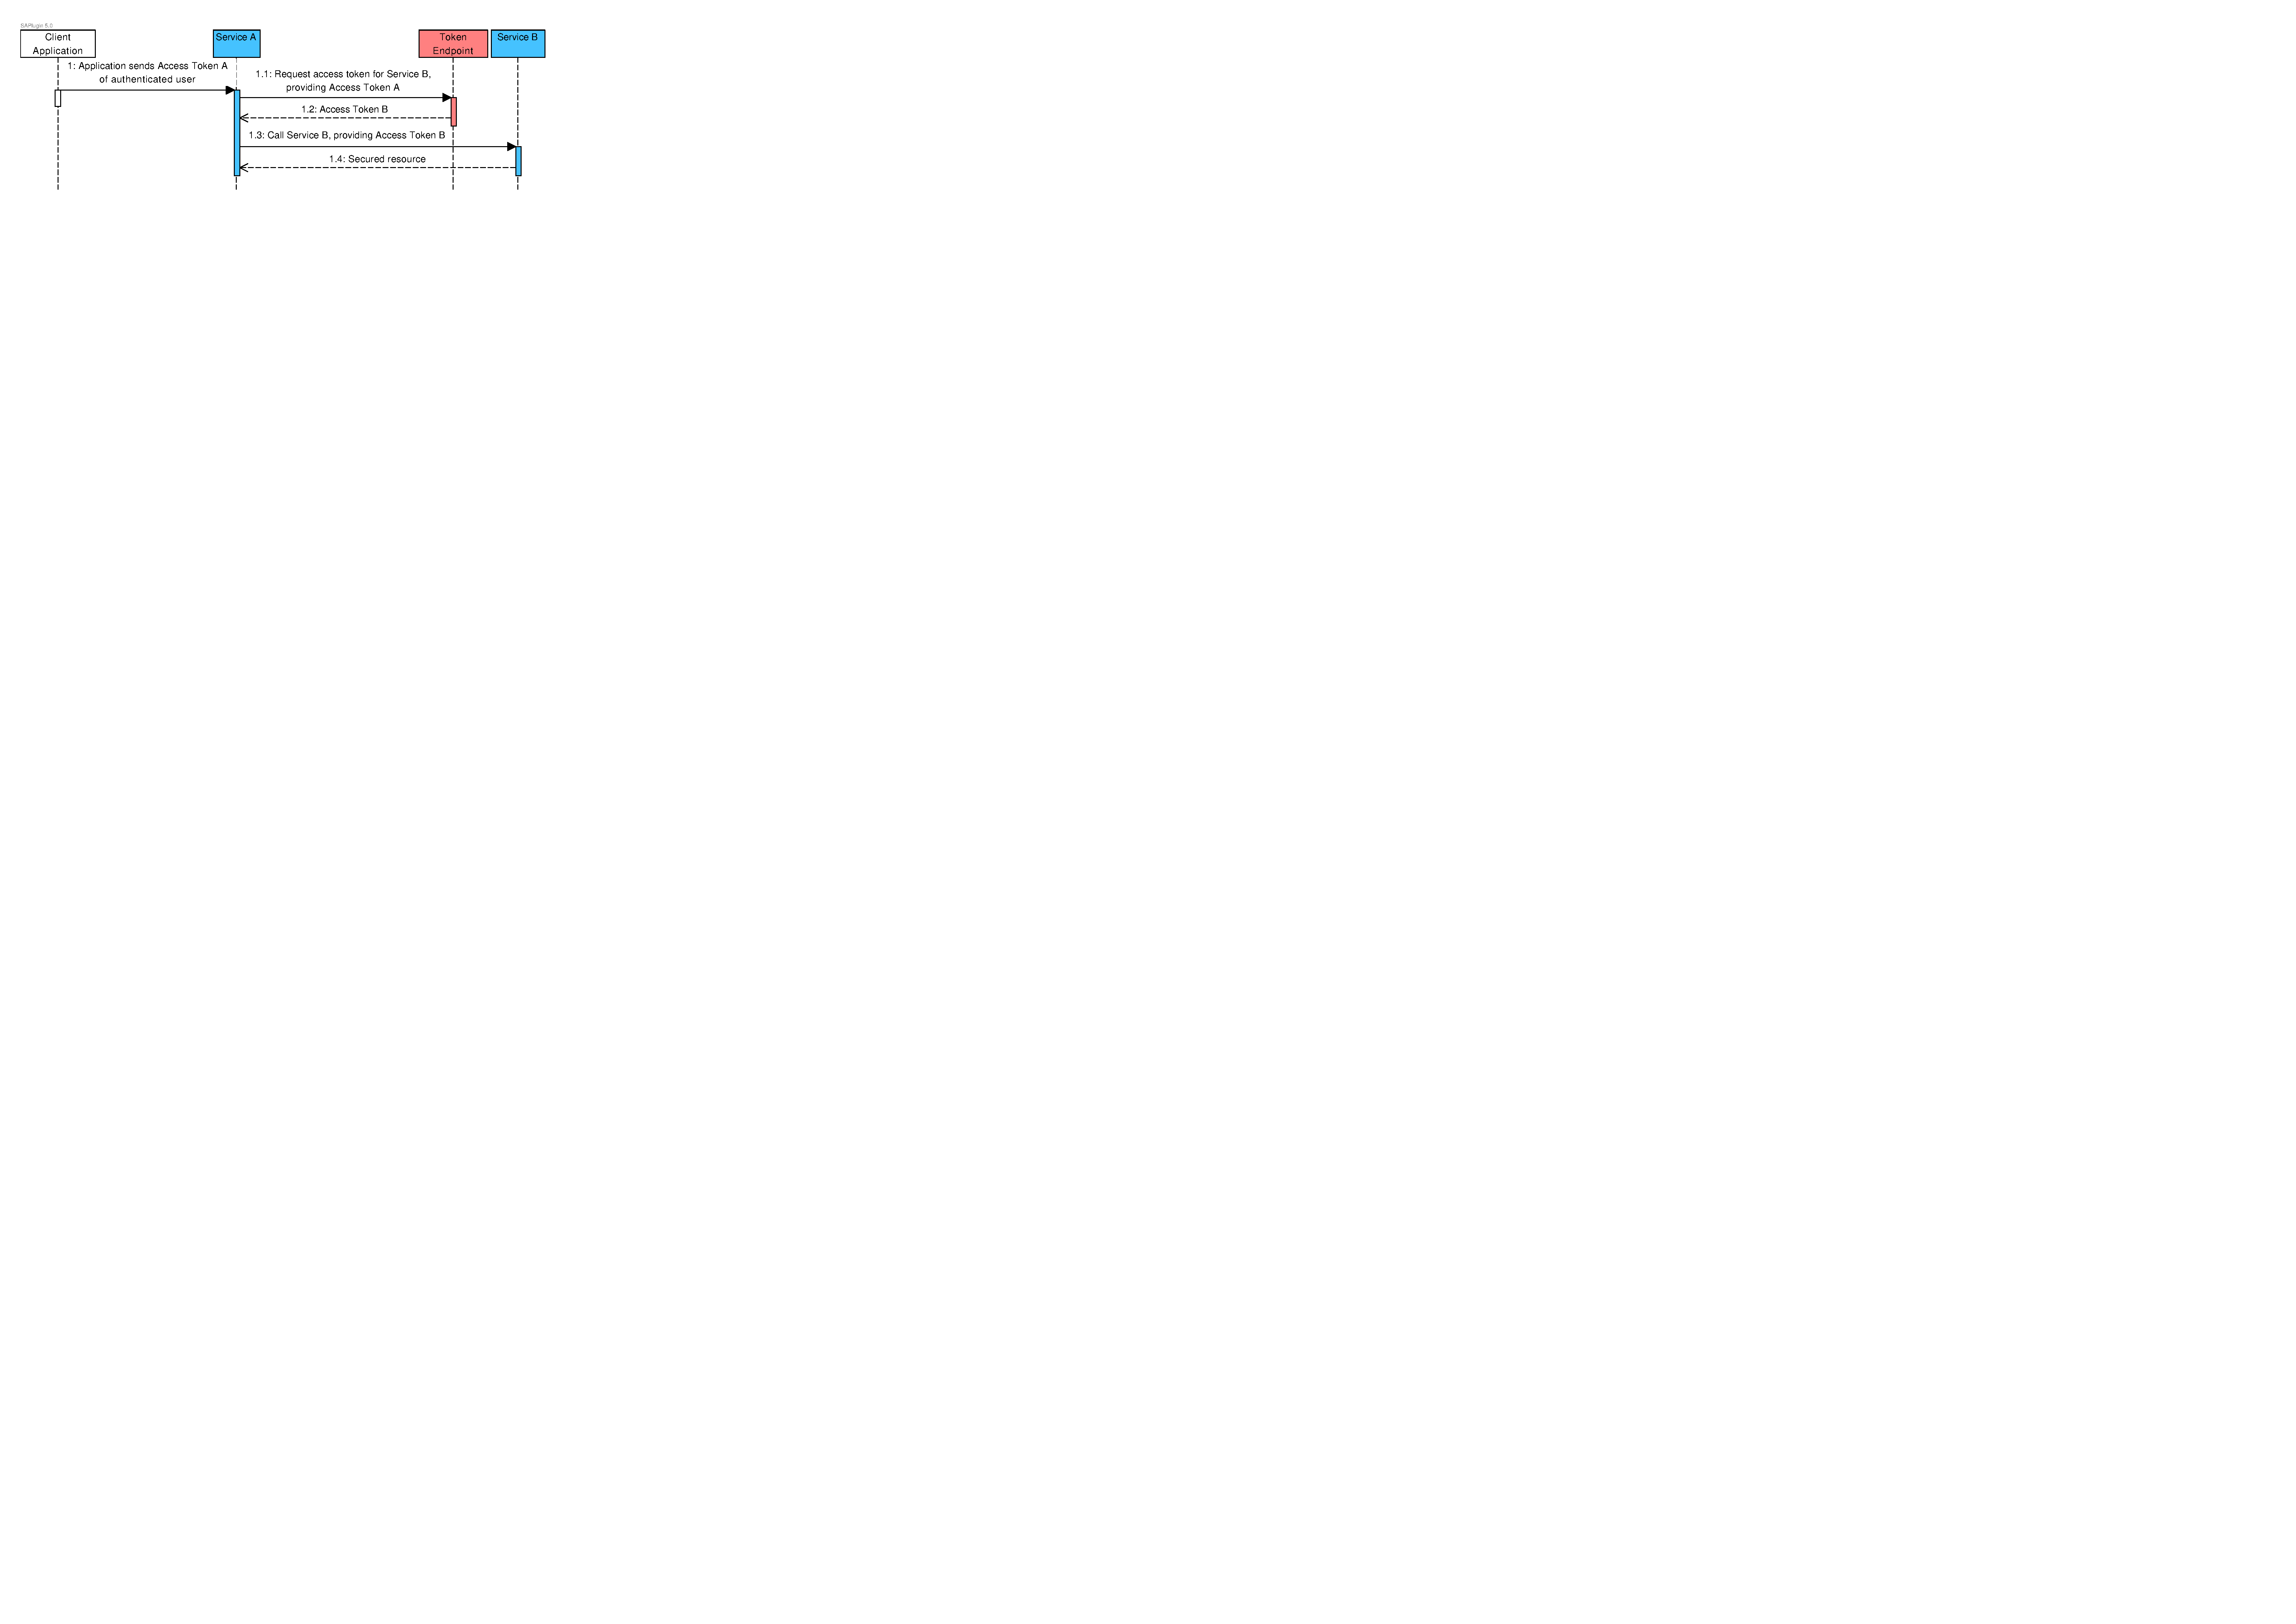
\includegraphics[width=1.0\textwidth]{images/macaroons-solid/InteractionDiagram-OBO-Flow.pdf}
    \caption{OAuth On-Behalf-Of flow}
    \label{fig:obo-flow}
\end{figure}

\noindent Concretely, the following steps are executed:
\begin{enumerate}
    \item The client has authenticated the user and has an access token bound to this user's identity (Access Token A)
    \item The client sends a request to Service A, providing Access Token A
    \item Service A requests an access token for Service B on behalf of itself, providing Access Token A as part of the request
    \item The Token Endpoint generates an access token, B, and returns it
    \item Service A calls Service B, including Access Token B in the request
    \item Service B returns the secured resource
\end{enumerate}
\noindent Although this method functionally works, it has a number of important limitations in a decentralized environment. The main limitation is that this flow relies heavily on the Token Endpoint to generate new tokens every time an access token needs to be delegated. This creates a bottleneck when such tokens must often be generated, and makes the system more centralized. The next section will look into a different token system that resolves this issue.

\subsection{Decentralized delegation of access tokens using macaroons}
Macaroons have a number of interesting properties that make them suitable as an access token for realizing decentralized delegation of access token. Concretely, this decentralized delegation means that a Service A can delegate its access token to Service B, without having to contact the Token Endpoint for obtaining a new token.

Delegation of macaroons works out-of-the-box, because by default macaroons are not bound to a specific client (nor is a proof-of-possession mechanism employed). Such restrictions must be added by adding caveats that restrict the macaroon's usage to a specific application (and a specific user, target resource, etc.). By default, macaroons can also be extended with additional caveats. This enables a service that wishes to delegate its access token to add additional constraints on the token usage (such as making it usable only once, adding a more strict time restriction, etc.).

Since Solid uses OAuth as its authentication mechanism, a new access token mechanism should be compatible with OAuth. Fortunately, macaroons have already been used in production systems as access and refresh tokens. The original macaroons paper discusses macaroons in the context of OAuth \citep[p.12]{macaroons}, and the ForgeRock AM 7 Access Management system supports the use of macaroons as access tokens in OAuth\footnote{See \url{https://backstage.forgerock.com/docs/am/7/oauth2-guide/oauth2-macaroons.html}}.

Realizing access delegation naively may lead to severe vulnerabilities, where tokens can be stolen. Therefore, delegation should be disabled by default by limiting a macaroon to a certain WebID (the application's WebID). An application that requests access delegation should include this information when requesting an access token, specifying the WebIDs of the third-party services. Figure \ref{fig:decentralized-delegation-macaroon} illustrates the flow of delegating an access token in Solid, in the context of an aggregator.

\begin{figure}[h]
    \centering
   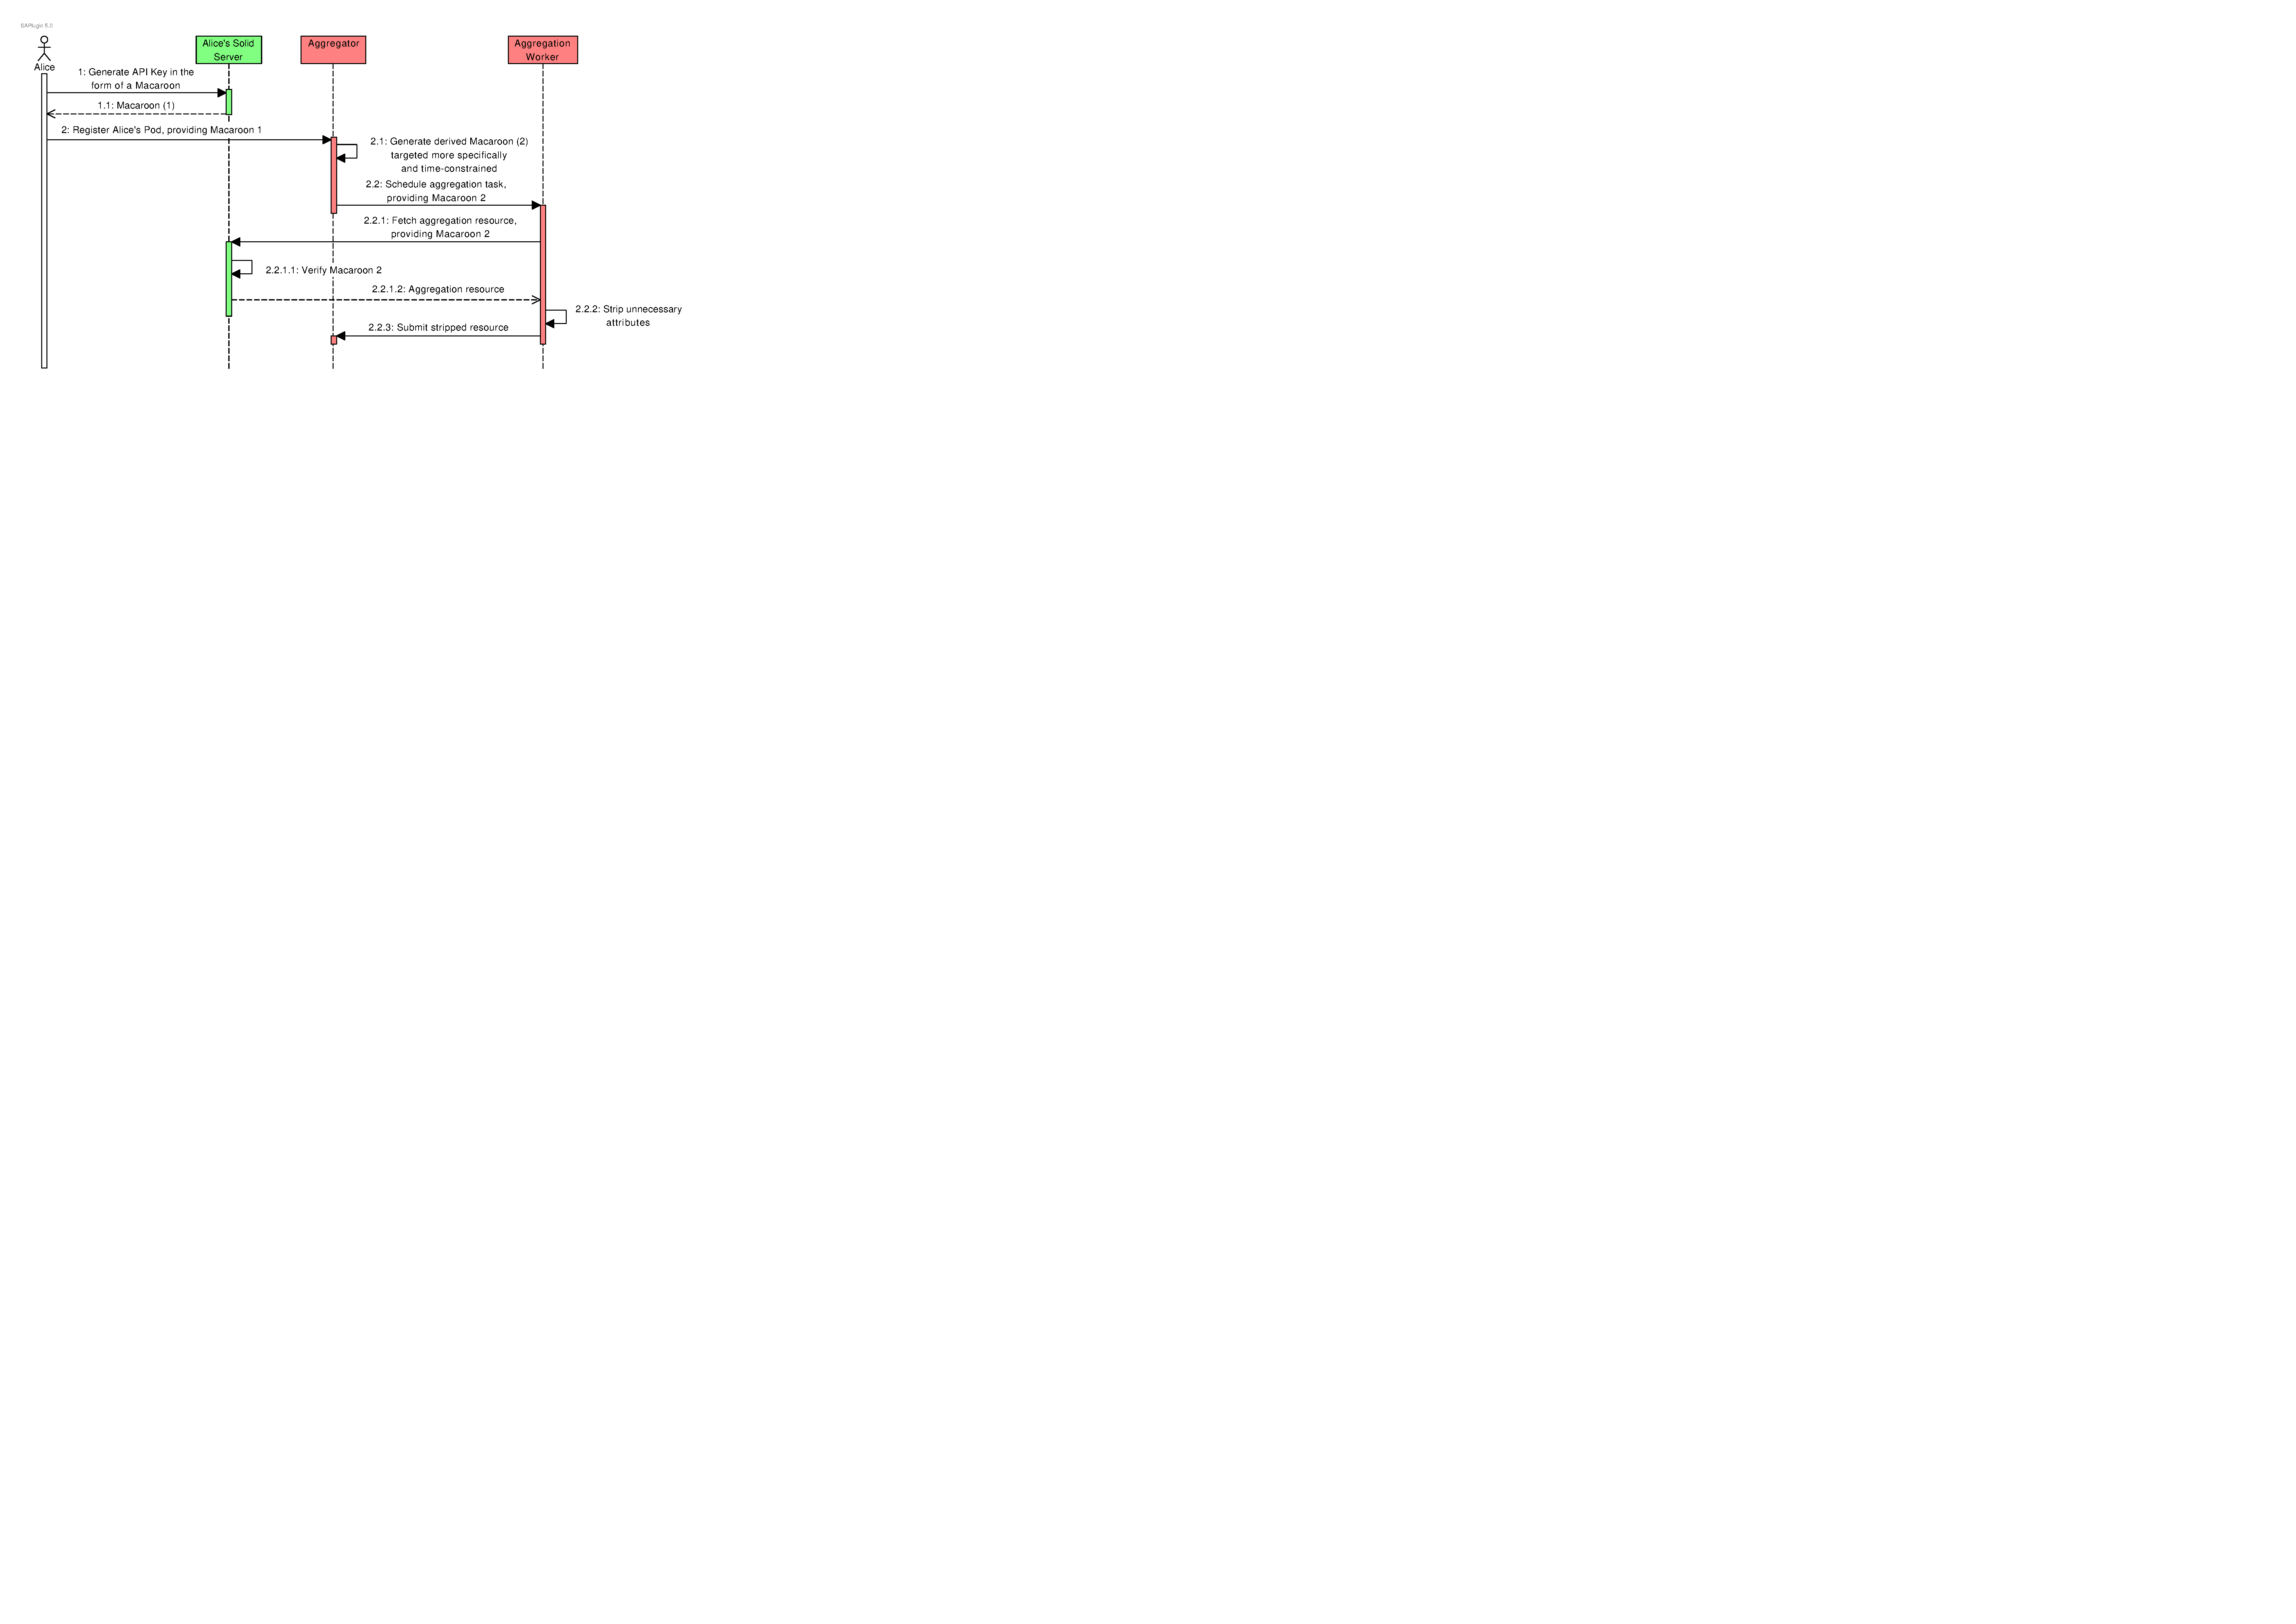
\includegraphics[width=1.0\textwidth]{images/macaroons-solid/InteractionDiagram-Decentralized-Delegation-of-Macaroon.pdf}
    \caption{Decentralized Delegation of Macaroon in Solid Data Aggregator}
    \label{fig:decentralized-delegation-macaroon}
\end{figure}

\noindent As can be seen in figure \ref{fig:decentralized-delegation-macaroon}, the \texttt{Aggregator} component does not need to contact \texttt{Alice's Solid Server} (the token endpoint) to generate a new macaroon to pass to the \texttt{AggregationWorker}. 

Apart from not having to contact the token endpoint, the usage of macaroons in this context provides additional benefits as well. 
Firstly, when the \texttt{Aggregator} derives a new macaroon to delegate, this can be confined to the concrete request very precisely. For instance, the derived macaroon can be limited to a specific resource (such as \texttt{health-data/01042022.json}), to a specific method (such as \texttt{GET}), and within a very specific time frame (such as in the next sixty seconds). 

Additionally, combining macaroons with the privacy filters proposed in chapter \ref{cha:privacy-filters} also allows confining the tokens to a specific privacy level. In this way, a Solid server can rewrite the data to strip sensitive personal information even before passing it to the aggregator. This decreases the reliance on the aggregator to correctly perform such operations, increasing the trust level of aggregators. Furthermore, by already stripping a number of attributes in the Solid server, the system load of the aggregator is decreased since it must receive less data.

Finally, macaroons also prove to be a very safe and secure method of handing out API keys. Traditionally, API keys (whether they are in the form of bearer tokens, \gls{JWT}s or other token types) require either extensive bookkeeping (in the case of bearer tokens) or verifying signatures (in the case of \gls{JWT}s) to verify whether they are valid. However, none of them offer good anti-theft mechanisms apart from token revocation. Unfortunately, such token thefts can often go unnoticed. However, since macaroons can be easily confined to an identifier (such as an IP address), they offer more extensive protection mechanisms. They also don't come with the downside of extensive bookkeeping for bearer tokens (since authorization limitations are embedded in the macaroon), and can be revoked easily by adding a caveat to check the token identifier in a revocation list. Concretely, the content of Macaroon 1 and Macaroon 2 would look like the macaroons presented in table \ref{table:delegated-macaroon}.

\begin{table}[!htb]
   \centering
    \begin{subtable}{.4\linewidth}
      \centering
        \begin{tabular}{|l|}
        \hline
        RANDOM\_NONCE                                       \\ \hline
        location https://pods.org                           \\ \hline
        identifier 3ff99779-720e...                         \\ \hline
        cid user = alice                                    \\ \hline
        cid operation = read                                \\ \hline
        cid target = /health                                \\ \hline
        cid expiry = 01-01-2024                             \\ \hline
        cid webid = https://agg.com/...                     \\ \hline
        cid privacy\_level = 3                              \\ \hline
        sig ec35a6224861d2f83542c7f2...                     \\ \hline
        \end{tabular}
        \caption{Aggregator macaroon}
    \end{subtable}%
    \begin{subtable}{.6\linewidth}
      \centering
        \begin{tabular}{|l|}
        \hline
        RANDOM\_NONCE                                       \\ \hline
        location https://pods.org                           \\ \hline
        identifier 3ff99779-720e...                         \\ \hline
        cid user = alice                                    \\ \hline
        cid operation = read                                \\ \hline
        cid target = /health/010422.json                    \\ \hline
        cid expiry = 01-06-2022 17:04:02                    \\ \hline
        cid webid = https://agg.com/...                     \\ \hline
        cid privacy\_level = 3                              \\ \hline
        cid ip = 193.190.253.145                            \\ \hline
        sig b7da027f072ce6f5a64c35ab...                     \\ \hline
        \end{tabular}
        \caption{Derived macaroon}
    \end{subtable} 
    \caption{Illustration of macaroon delegation}
    \label{table:delegated-macaroon}
\end{table}

\chapter{Evaluation}
\label{cha:evaluation}
This chapter evaluates the solutions proposed in this thesis. The first section discusses some theoretical limitations of the proposed solutions. The second section will then benchmark the performance of the developed prototypes, to verify the impact of the proposed solutions compared to a vanilla version of the \acrlong{CSS}. Finally, the last section validates the proposed solutions in the context of the use cases presented in section \ref{sec:usecases}.

\section{Theoretical limitations}
\subsection{Privacy filters}
Privacy filters are a mechanism to dynamically rewrite resources to improve privacy. The currently proposed solution comes with a number of limitations, which are listed below.\\

\noindent \textbf{No write-back} Data is modified on a per-request basis, where certain attributes could be changed or removed. In the proposed solution, no mapping of this is kept (which might not even always be possible). As such, when an application modifies this data and tries to write it back, there is no way to reconcile these two versions. In the context of an aggregator that only reads data, this does not pose a problem, but it limits the use of privacy filters in other contexts.\\

\noindent \textbf{Lack of domain knowledge} Often, domain knowledge is needed to construct useful transformations. For example, to strip out the user's name while keeping other names, it is necessary to know the user's name. Similarly, when information is made less specific (for example, replacing "Colruyt" with "supermarket"), it is important to have a mapping of such strings. This means that either users must add some necessary information to the privacy filter configuration files, or that localized filters (for example, containing information about Belgian supermarkets) should be sourced from somewhere.\\

\noindent \textbf{Only structured data} Since privacy filters, in the proposed solution, work on a per-attribute basis, they do not support performing transformations on unstructured data. For such data, more sophisticated techniques ought to be used (such as machine learning models). Techniques for this already exist (such as \citet{privacy-unstructured-scoring} and \citet{privacy-preserving-unstructured}), but are complex to integrate and computationally very expensive to run on a per-request basis. \\

\noindent \textbf{Data linkage} Privacy filters only work on a single resource/dataset. However, very often de-anonymization happens because multiple datasets are linked together. Privacy filter only provide limited protection against such information disclosures since resources are transformed on a one-by-one basis without looking at the complete picture. Fetching multiple resources from a single pod may disclose information that should have been filtered out.

\subsection{Macaroons as access tokens}
While macaroons offer a number of advantages as access tokens, there is no free lunch. Like any other solution, macaroons also come with disadvantages. This subsection lists a number of the most important disadvantages.\\

\noindent \textbf{Verification requires trust} Verification of a macaroon happens by recomputing the signature of the macaroon, and confirming that the calculated signature matches the signature present in the macaroon. The first computed signature is computed based on the random nonce present in the macaroon and the \textit{root key}. As such, this implies that a service that wishes to verify a macaroon must be in possession of the root key (or delegate verification to another service that possesses the root key). 

When the target service (the service that receives a request) is running on the same server as the service handing out the macaroon, this does not pose a problem. The \acrlong{CSS}, for example, works like this. However, scenarios were this is not the case are not impossible. For those scenarios, a mechanism must be devised where the verification is either delegated, or the service is trusted and receives the root key.\\

\noindent \textbf{Caveats are not standardized} The original macaroons paper defined what a caveat is and how macaroons are composed, but it did not define a language to express caveats in. Neither does it define in what way macaroons should be serialized for transportation over the internet (such as base64). Due to this limitation, multiple, incompatible libraries exist for using macaroons. Furthermore, since the expression of caveats is not even dependent on the used library, services that require third-party attestations must make sure that caveats are expressed in the same way (since a discharge macaroon may also contain caveats). 

Therefore, the Solid specification should be extended with definitions of which serialization should be used, and a unified way of representing caveats (for example, in \gls{RDF}) must be defined. These decisions have an impact on which existing libraries can be used, or whether custom libraries must be developed.

%\subsection{Additional limitations}

\section{Evaluation of the performance}
This section discusses a number of benchmarking experiments that have been performed to evaluate the performance of the proposed middleware. The first experiment focuses on the overhead of running privacy filters on top of Solid, comparing the processing time with and without privacy filters. The second experiment measures the performance improvement of using macaroons instead of using \gls{DPoP}-based tokens. 

\subsection{Experiments set-up}
\subsubsection{Experiment 1: Overhead of privacy filters}
The first experiment performed focuses on the overhead of running privacy filters on top of Solid. Therefore, a number of requests are sent to the Solid server, comparing the times it takes to fulfill the request between a version with privacy filters (running the privacy-enhancing middleware) and a vanilla version. To provide an overview of the performance overhead that is general enough (and not tied to one specific resource), requests are made to multiple resources, of different data types, content representations, ...

\subsubsection{Experiment 2: Performance improvement of macaroons compared to DPoP}

\subsection{Results}


\section{Validation of use cases}
\subsection{Exercise data}
\subsection{Personal finance}
\subsection{Aggregated view on personal health data streams}

\section{Conclusion of evaluation}

\chapter{Conclusion}
\label{cha:conclusion}
\section{Overview}


\section{Future work}

\begin{futurework}\label{fw:homomorphic-encryption}
\textbf{- Homomorphic encryption in Solid} Homomorphic encryption is an encryption technology that allows for mathematical operations on the ciphertext. It was discussed in section \ref{sec:enc-db}. Homomorphic encryption is a computationally expensive yet promising technology for securely aggregating data. Thus, in the context of privacy-aware technologies for Solid, it could be very interesting.  For example, a possible use case could be an application that collects salaries from a number of pods, and then gives back an encrypted answer to each pod containing the average salary. In this way, interesting insights can be gained without sacrificing personal information. However, this method also lacks somewhat in the need for a centralized party that performs the aggregation - it is not fully decentralized. Whether this is problematic depends heavily on the concrete use case. Additionally, some coordination is needed between the pods beforehand to make sure that the necessary data is encrypted in the same manner. Future research could investigate a potential implementation of a secure data aggregator for Solid based on homomorphic encryption schemes.
\end{futurework}

\begin{futurework}\label{fw:mpc}
\textbf{- \gls{MPC} in Solid} \acrlong{MPC} is a cryptographic technique that allows for securely performing computations on data, without sharing this data between parties. While at first glance this might seem similar to FW \ref{fw:homomorphic-encryption}, there are some major differences. Firstly, in the case of the homomorphic encryption, there was a single central party that performed the computation. In the case of \gls{MPC}, however, this computation is entirely decentralized and happens on the parties themselves; data is never shared or exposed. Secondly, \gls{MPC} can compute virtually any computable function by making use of its garbled circuits. Homomorphic encryption, on the other hand, is limited to the mathematical operations of addition and multiplication of the ciphertexts. This has many advantages as the \gls{MPC} scenario clearly allows for much broader applications. However, in the homomorphic encryption scenario, only very few modifications to the Solid protocol would be required as the bulk of the work would happen in the party that performed the aggregation by requesting encrypted data from multiple pods. However, as \gls{MPC} does not share any data and computations happen locally, an implementation of \gls{MPC} in Solid would require many additions to the Solid protocol. Developing an architecture an improved specification for Solid could thus be very interesting future research, with many possible applications.
\end{futurework}

\begin{futurework}\label{fw:privacy-levels}
\textbf{- Privacy levels} Currently, this thesis has proposed a number of so-called \textit{privacy levels} (see section \ref{sec:privacylevels}) which form a granular way to determine how much data may be handed over to an untrusted application. However, this was only a practical proposal lacking a rigorous definition. Future research could investigate possible ways to define privacy levels more rigorously, for example by finding some sort of leakage metric that determines the maximum leakage of data under a certain privacy level.
\end{futurework}

\begin{futurework}\label{fw:abe}\textbf{- \acrlong{ABE}}
Section \ref{sec:attacker-model} highlighted a honest-but-curious adversary model where applications are untrusted. However, an attacker model where the roles are reversed is also possible. This would be a scenario where the applications are highly trusted, but the Solid pod is stored at a third party and there is no way to verify that there are no vulnerabilities in the server source code. As such, this implies an active attacker that can deviate from the protocol and actively tries to bypass the Solid server's authentication and authorization mechanisms. Effectively, this implies that the attacker can access resources to which it should not have access according to the \gls{ACL}s as these resources can be stored on-disk. Should an attacker breach the server (for exampling, getting SSH access in some way), then he can read all resources stored on the server. 

A good solution to this problem would be encryption, which would obscure the data stored in the Solid pod, and only parties with a correct key could access the data. However, in the decentralized context of Solid, this is hard to achieve. Multiple applications need to access the same data, and access policies for resources can be complex. In addition, these access policies must also be dynamic, meaning that it must be possible for a user to withdraw an application's access to a resource.

A naive approach could use symmetric key encryption because of the high speed and computational efficiency, but this approach is lacking in this decentralized context as key management would be problematic. Since many access policies are possible, a key per policy would be required, which comes with a lot of overhead and bookkeeping (such as, knowing which key to use for which resource). Secondly, when access to a resource is withdrawn from a certain application, new keys must be generated, distributed to all applications with access to that resource, and the resource must be re-encrypted. All of this makes that symmetric key encryption is a bad fit for this requirement.

On the other hand, in chapter \ref{cha:analysis}, an analysis was made of \acrfull{ABE}. \Gls{ABE} could be a very effective method of reaching the stated goals; although some extra infrastructure would be required. Specifically, \gls{CP-ABE} offers many advantages in this context. First of all, key management is relatively straightforward. Because attributes are stored in private keys, every application only requires a single key per user. The access policies are independent of the distributed keys, facilitating key distribution. Secondly, \gls{CP-ABE} allows for very complex access policies per resource using threshold gates of attributes. These access policies are stored directly in the ciphertext, minimising their bookkeeping. Thirdly, the access policies can also be made dynamic. When the access requirements of a resource change, only the resource has to be re-encrypted with its new access policy. The private keys of all the applications do not need to be changed. However, because of the decentralized nature of \middleware{}, there are still some security challenges left. This section introduces a possible solution, which future research could investigate, extend, implement, and evaluate. This solution consists of a number of different phases, partially corresponding to the phases present in \gls{ABE}.

\textbf{Setup phase}
First, a security parameter is taken in, and a master and public key are generated. This public key is used for encrypting resources, the master key is used for generating private keys in the next step. 

In the second part of the setup phase, a private key is generated for every trusted client application. This step takes as input the public key, the master key, and a set of attributes that should be assigned to the client application. This step is then repeated for every trusted client application.

In the third step of the setup phase, the access policies are created. This part of the setup phase requires as input a mapping of resources to access policies. These access policies are embedded in the ciphertext of encrypted resources, and determine which attributes a private key must contain in order for it to be able to decrypt the ciphertext. Since these access policies can be subject to change, applications must request them before using these to encrypt a resource. However, this also introduces a possible vulnerability: if the access policies are stored in plaintext on the server, a malicious actor could modify them to make them trivially satisfied. Therefore, the access policies should bear some sort of digital signature, to attest their authenticity. Similarly, the public key should also bear the signature of a Certificate Authority, similar to SSL certificates, to allow clients to verify the authenticity of the public key. When these access policies are created for every resource, the resources are encrypted using the public key and the generated access policy.

After the setup phase is completed, the master key is handed over to the user, after which it is destroyed. 

\textbf{Key distribution}
Once the setup phase has finished, the Solid server has a number of private keys (one per client application). It is unsafe to store them on the untrusted Solid server. Therefore, the first time a client application connects to the Solid server, the client application must first fetch the private key. Afterwards, it is destroyed from the Solid server, making sure that in case of a breach no keys are leaked. This means that there is a certain time period when the Solid server is still vulnerable to leaking data of the user. However, typically, there is no time period when both data and the private key are stored on the Solid server. As such, the only real risk is when a breach goes undetected for a while. In this scenario, an attacker could read the private keys, and after a while when data starts flowing in, decrypt this data. 

\textbf{Encryption and decryption}
Once the setup phase and key distribution have been completed, trusted applications can begin interacting with encrypted resource containers. When an application requests a resource, it will receive an encrypted representation of this resource. The application can then use its private key to decrypt this resource, if its key satisfies the access policy of the resource.

On the other hand, encrypting resources is a bit more difficult. The encryption process has three inputs: the plaintext data, the public key and the access policy. The public key and access policy must be fetched from the Solid server where the resource will be stored. When the public key is fetched, the client application can verify its authenticity by checking that it has been digitally signed by a trusted Certificate Authority. It must then also verify the authenticity of the access policy. This can be done by decrypting the encrypted access policy, with a public key that it received. In this manner, it can verify that the access policy was encrypted with a private key, and as such that it is authentic. It can then encrypt the resource locally, and finally send the encrypted resource to the Solid server.
\end{futurework}



% Indien er bijlagen zijn:
%\appendixpage*          % indien gewenst
\appendix
\chapter{\middleware{} configuration and code}
\section{Privacy level mapping}
\label{appendix:privacy-levels}
In our example data transformations, four levels of increasing privacy are proposed, based partially on the \gls{GDPR} definition of sensitive personal data and on the types of identifiers defined in section \ref{sec:data-deid}. However, it is important to note that this is only a practical choice and forms a trade-off between granularity and necessary work (for setting up all the transformations required for a certain level). Privacy experts may have more valuable opinions on the correct number of privacy levels and how these should be communicated to a user. Future research could help to find a rigorous definition for these privacy levels, for example based on some leakage metric. This is elaborated in FW \ref{fw:privacy-levels}.\\

\noindent \textbf{Level 1: all data} No data transformations are applied, all data is passed on to the requesting application.\\

\noindent \textbf{Level 2: Removal of sensitive personal data} Sensitive personal data, as defined by the GDPR \citep{GDPR}, is removed from the dataset. This includes data consisting of racial or ethnic origin, political opinions, religious or philosophical beliefs, etc. Thus, the tactic \textit{Remove} is applied to all data elements matching this definition.\\

\noindent \textbf{Level 3: Pseudonymization/generalisation of direct identifiers} Since level 3 is a stronger version of level 2, sensitive personal data is removed first. Additionally, direct personal identifiers are pseudonymized or generalized/perturbed. Concretely, the tactics \textit{Pseudonym}, \textit{Encrypt}, \textit{Perturbation}, ... may be applied here, depending on the specific data attribute. Examples are the replacement of names by placeholders, the perturbation or adding a placeholder for birth dates (such that the exact date is obscured, but the age is still correct), the removal of street names and numbers while keeping larger geographic areas such as cities, etc. This makes the data still relatively accurate, while direct identification of the user is made impossible.\\

\noindent \textbf{Level 4: Pseudonymization/generalisation of (in)direct identifiers} In addition to direct identifiers, also indirect identifiers are now modified or removed. The same \gls{PETs} and tactics are used, but are now applied more strictly and to more data attributes. For example, when perturbing birth dates, now the exact age is not kept exactly, but it is changed to a range within the exact age. Cities may also be perturbed when possible, but keeping for example the province or state. Other indirect identifiers such as genders may also be modified or removed.

\section{Privacy Filter JSON Schema}
\label{appendix:privacy-filter-jsonschema}

\begin{code}
\inputminted[linenos,tabsize=2,breaklines]{json}{code/privacy-filter-json-schema.json}
\caption{JSON Schema describing the lay-out of privacy filter configuration files}
\label{listing:privacy-filter-jsonschema}
\end{code}
\section{Example Privacy Filter: KBC Transaction Data}
\label{appendix:privacy-filter-kbc}

\begin{code}
\inputminted[linenos,tabsize=2,breaklines]{json}{code/kbcbank-filter.json}
\caption{Example configuration file for a privacy filter in JSON, for the KBC Transaction Data datascheme. Fields are specified in JSONPath.}
\label{listing:privacy-filter-kbc}
\end{code}
\section{Dependency injection configuration for CSS}
\label{appendix:css-config}

\begin{code}
\inputminted[linenos,tabsize=2,breaklines]{json}{code/css-config.json}
\caption{JSON-LD specifying dependency injection of \middleware{} into \acrshort{CSS}}
\label{listing:css-config}
\end{code}
\section{Transformations performed in evaluation}
\label{appendix:performed-transformations}

\begin{code}
\inputminted[linenos,tabsize=2,breaklines]{json}{code/applied-transformations.json}
\caption{Transformations performed in evaluation}
\label{listing:performed-transformations}
\end{code}


\section{Community Solid Server Architecture}
\label{appendix:css-architecture}
\begin{figure}[h]
   \centering
   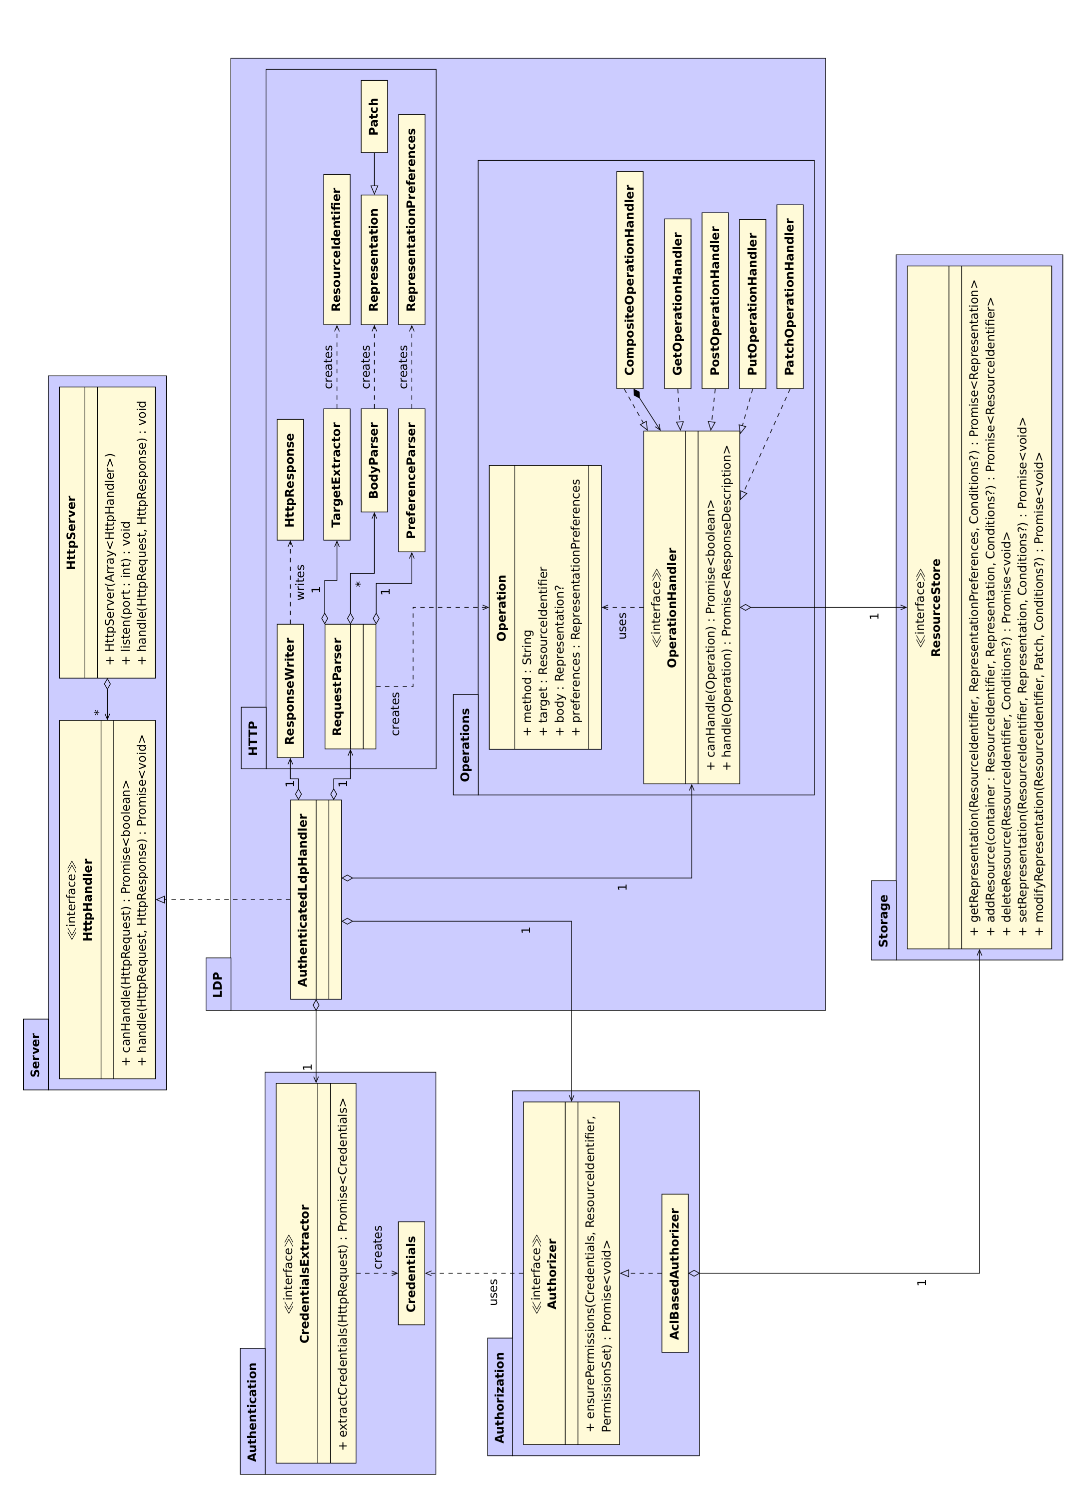
\includegraphics[width =0.9\textwidth]{appendices/solid-architecture/solid-architecture-v1-3-0-overview.pdf}
 \caption{Overview of the Community Solid Server architecture, by \citet{solid-diagram}}
 \label{fig:solid-arch}
\end{figure}
%%%% WARNING %%%
%%% This file was automatically generated by SAPlugin,
%%% and will be overwritten next time.

% macro for maximum width and height
\makeatletter\def\maxwidth#1{\ifdim\Gin@nat@width>#1 #1\else\Gin@nat@width\fi}\makeatother
\makeatletter\def\maxheight#1{\ifdim\Gin@nat@height>#1 #1\else\Gin@nat@height\fi}\makeatother


\graphicspath{appendices/architecture/images/}
%%%%%%%%%%%%%%%%%%%%%%%%%%%%%%%%%%%%%%%%%%%%%%%%%%%%
%%% CS
%%%%%%%%%%%%%%%%%%%%%%%%%%%%%%%%%%%%%%%%%%%%%%%%%%%%
\chapter{Client-server view (UML Component Diagram)}
\minilof{}






%%% DataAnonymizer Component Diagram (656.0x257.0)

\begin{figure}[!htp]
  \centering
  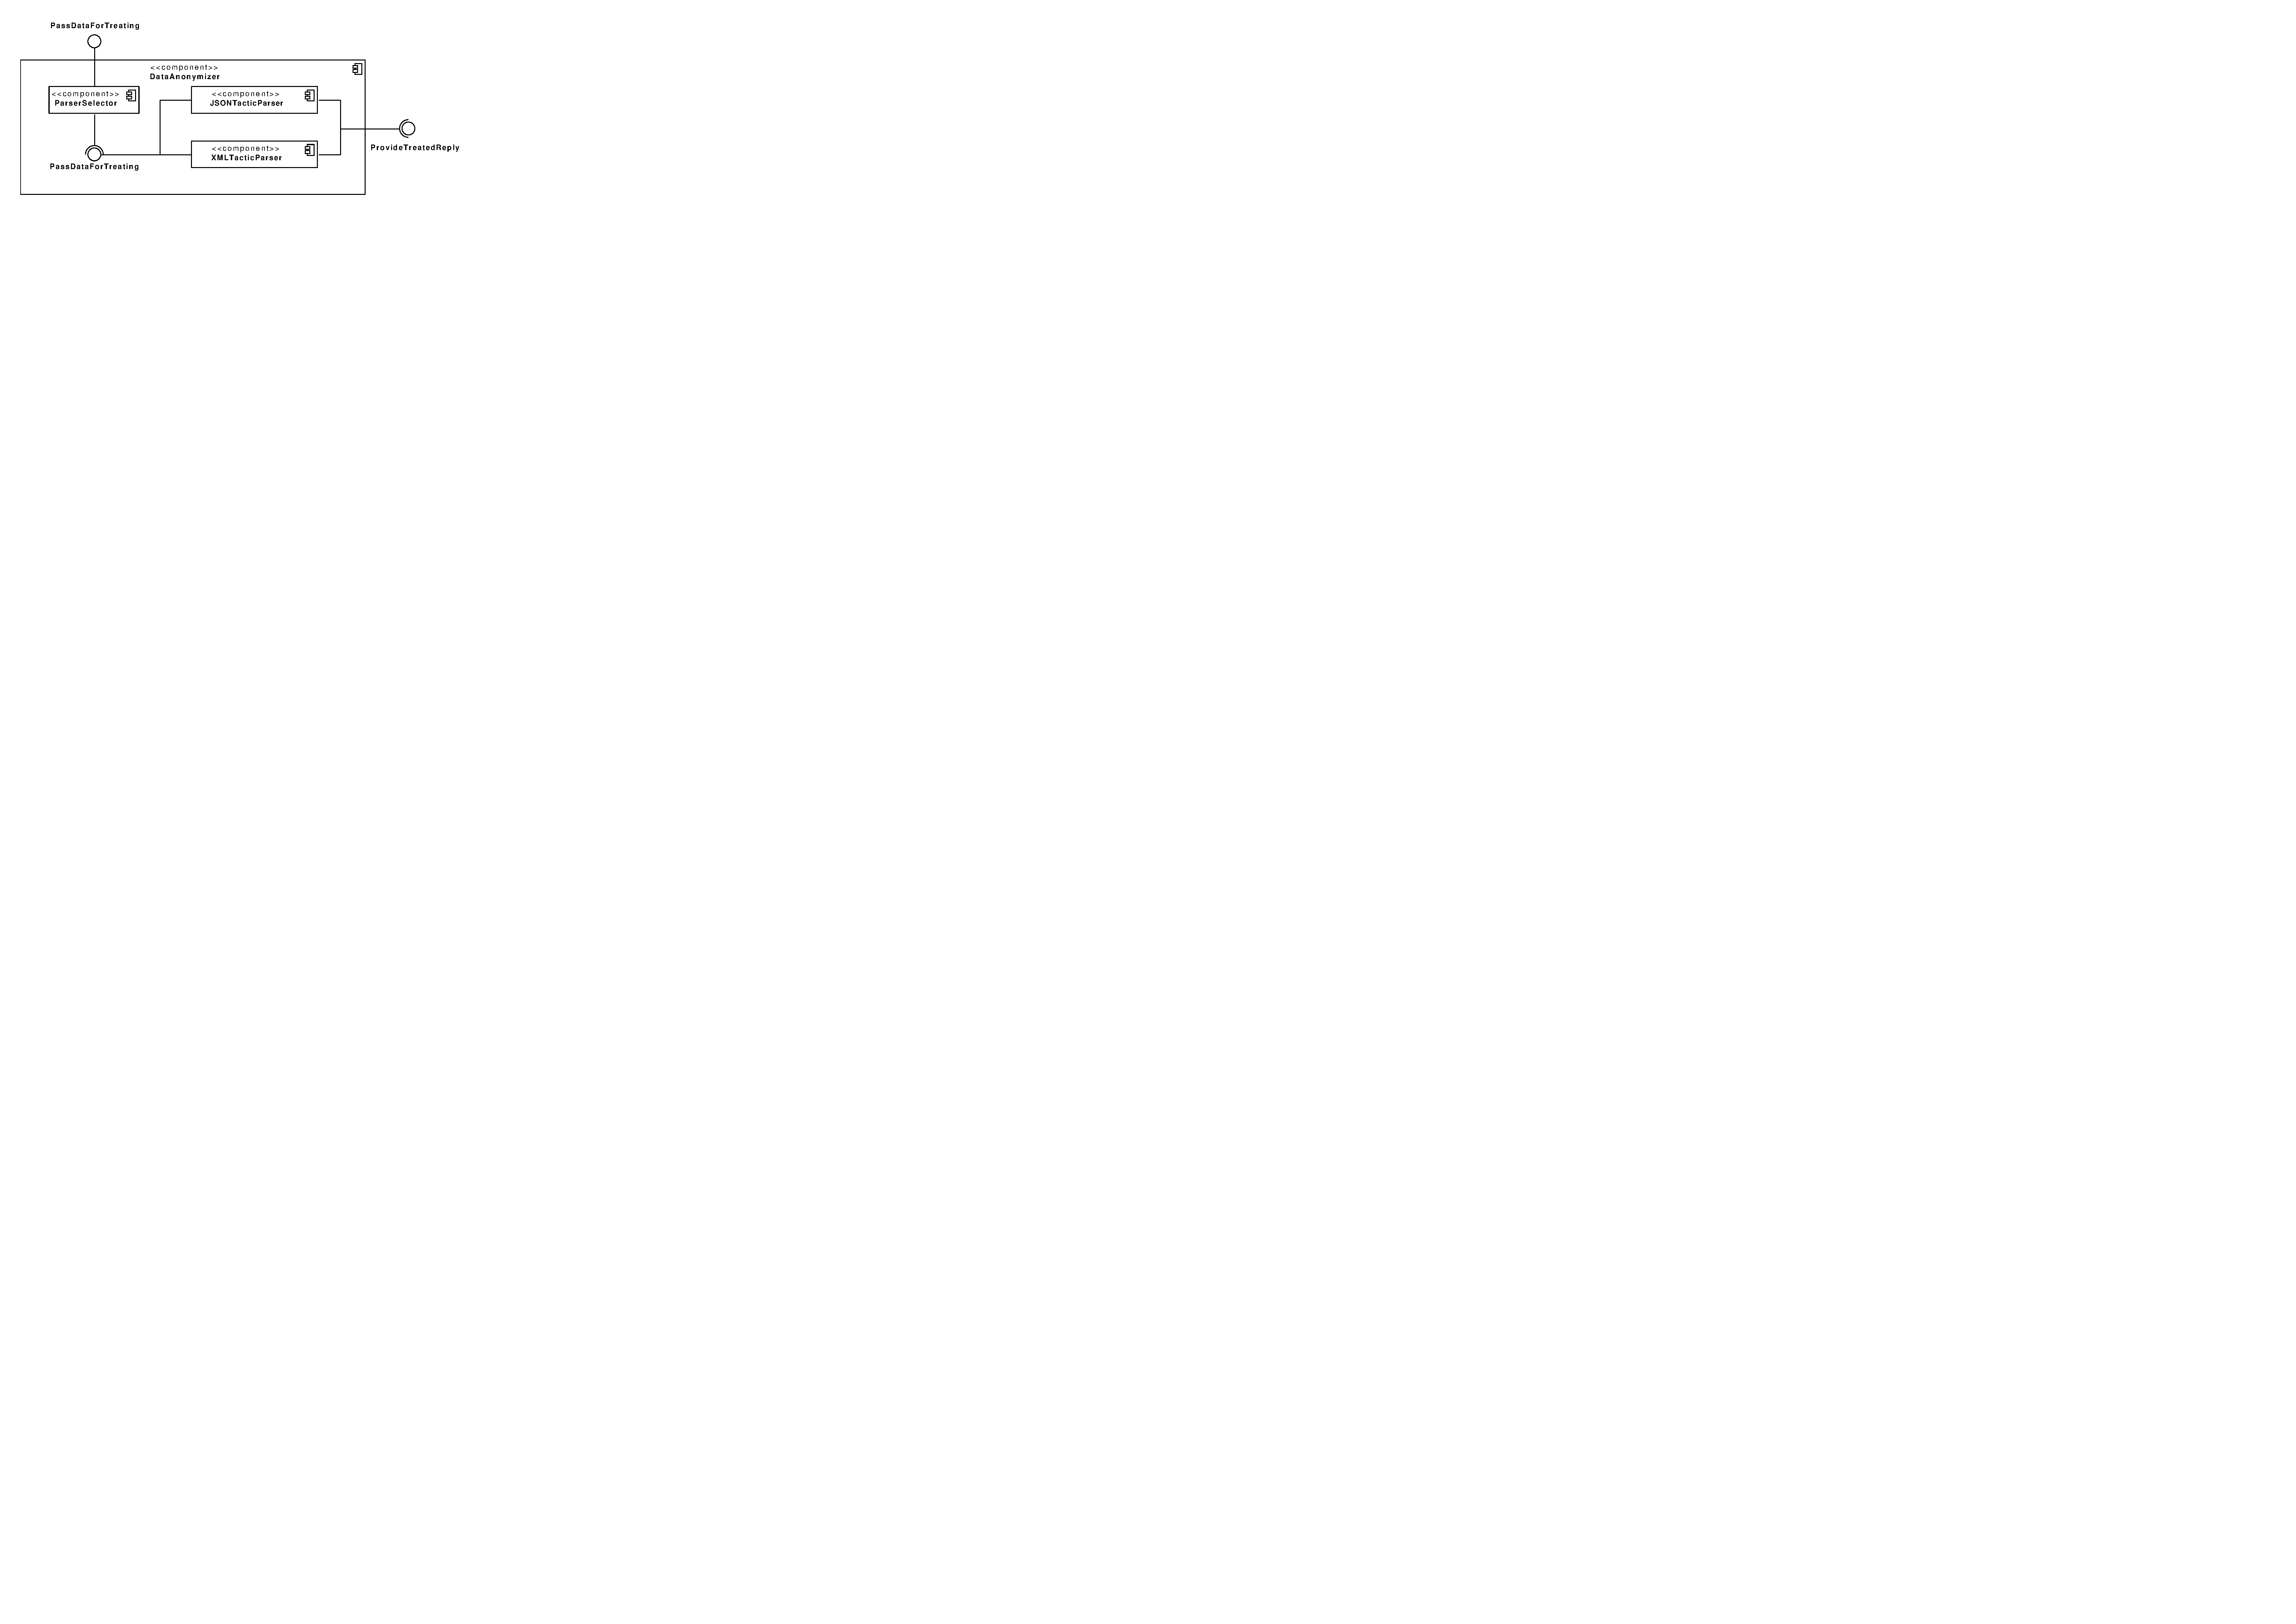
\includegraphics[width=\maxwidth{\textwidth}]{appendices/architecture/images/ComponentDiagram-DataAnonymizer-Component-Diagram.pdf}
  \caption[DataAnonymizer Component Diagram]{DataAnonymizer Component Diagram \label{diag:Component:DataAnonymizerComponentDiagram}}
\end{figure}

%%% DataTreatmentHandler Component Diagram (836.0x298.0)

\begin{figure}[!htp]
  \centering
  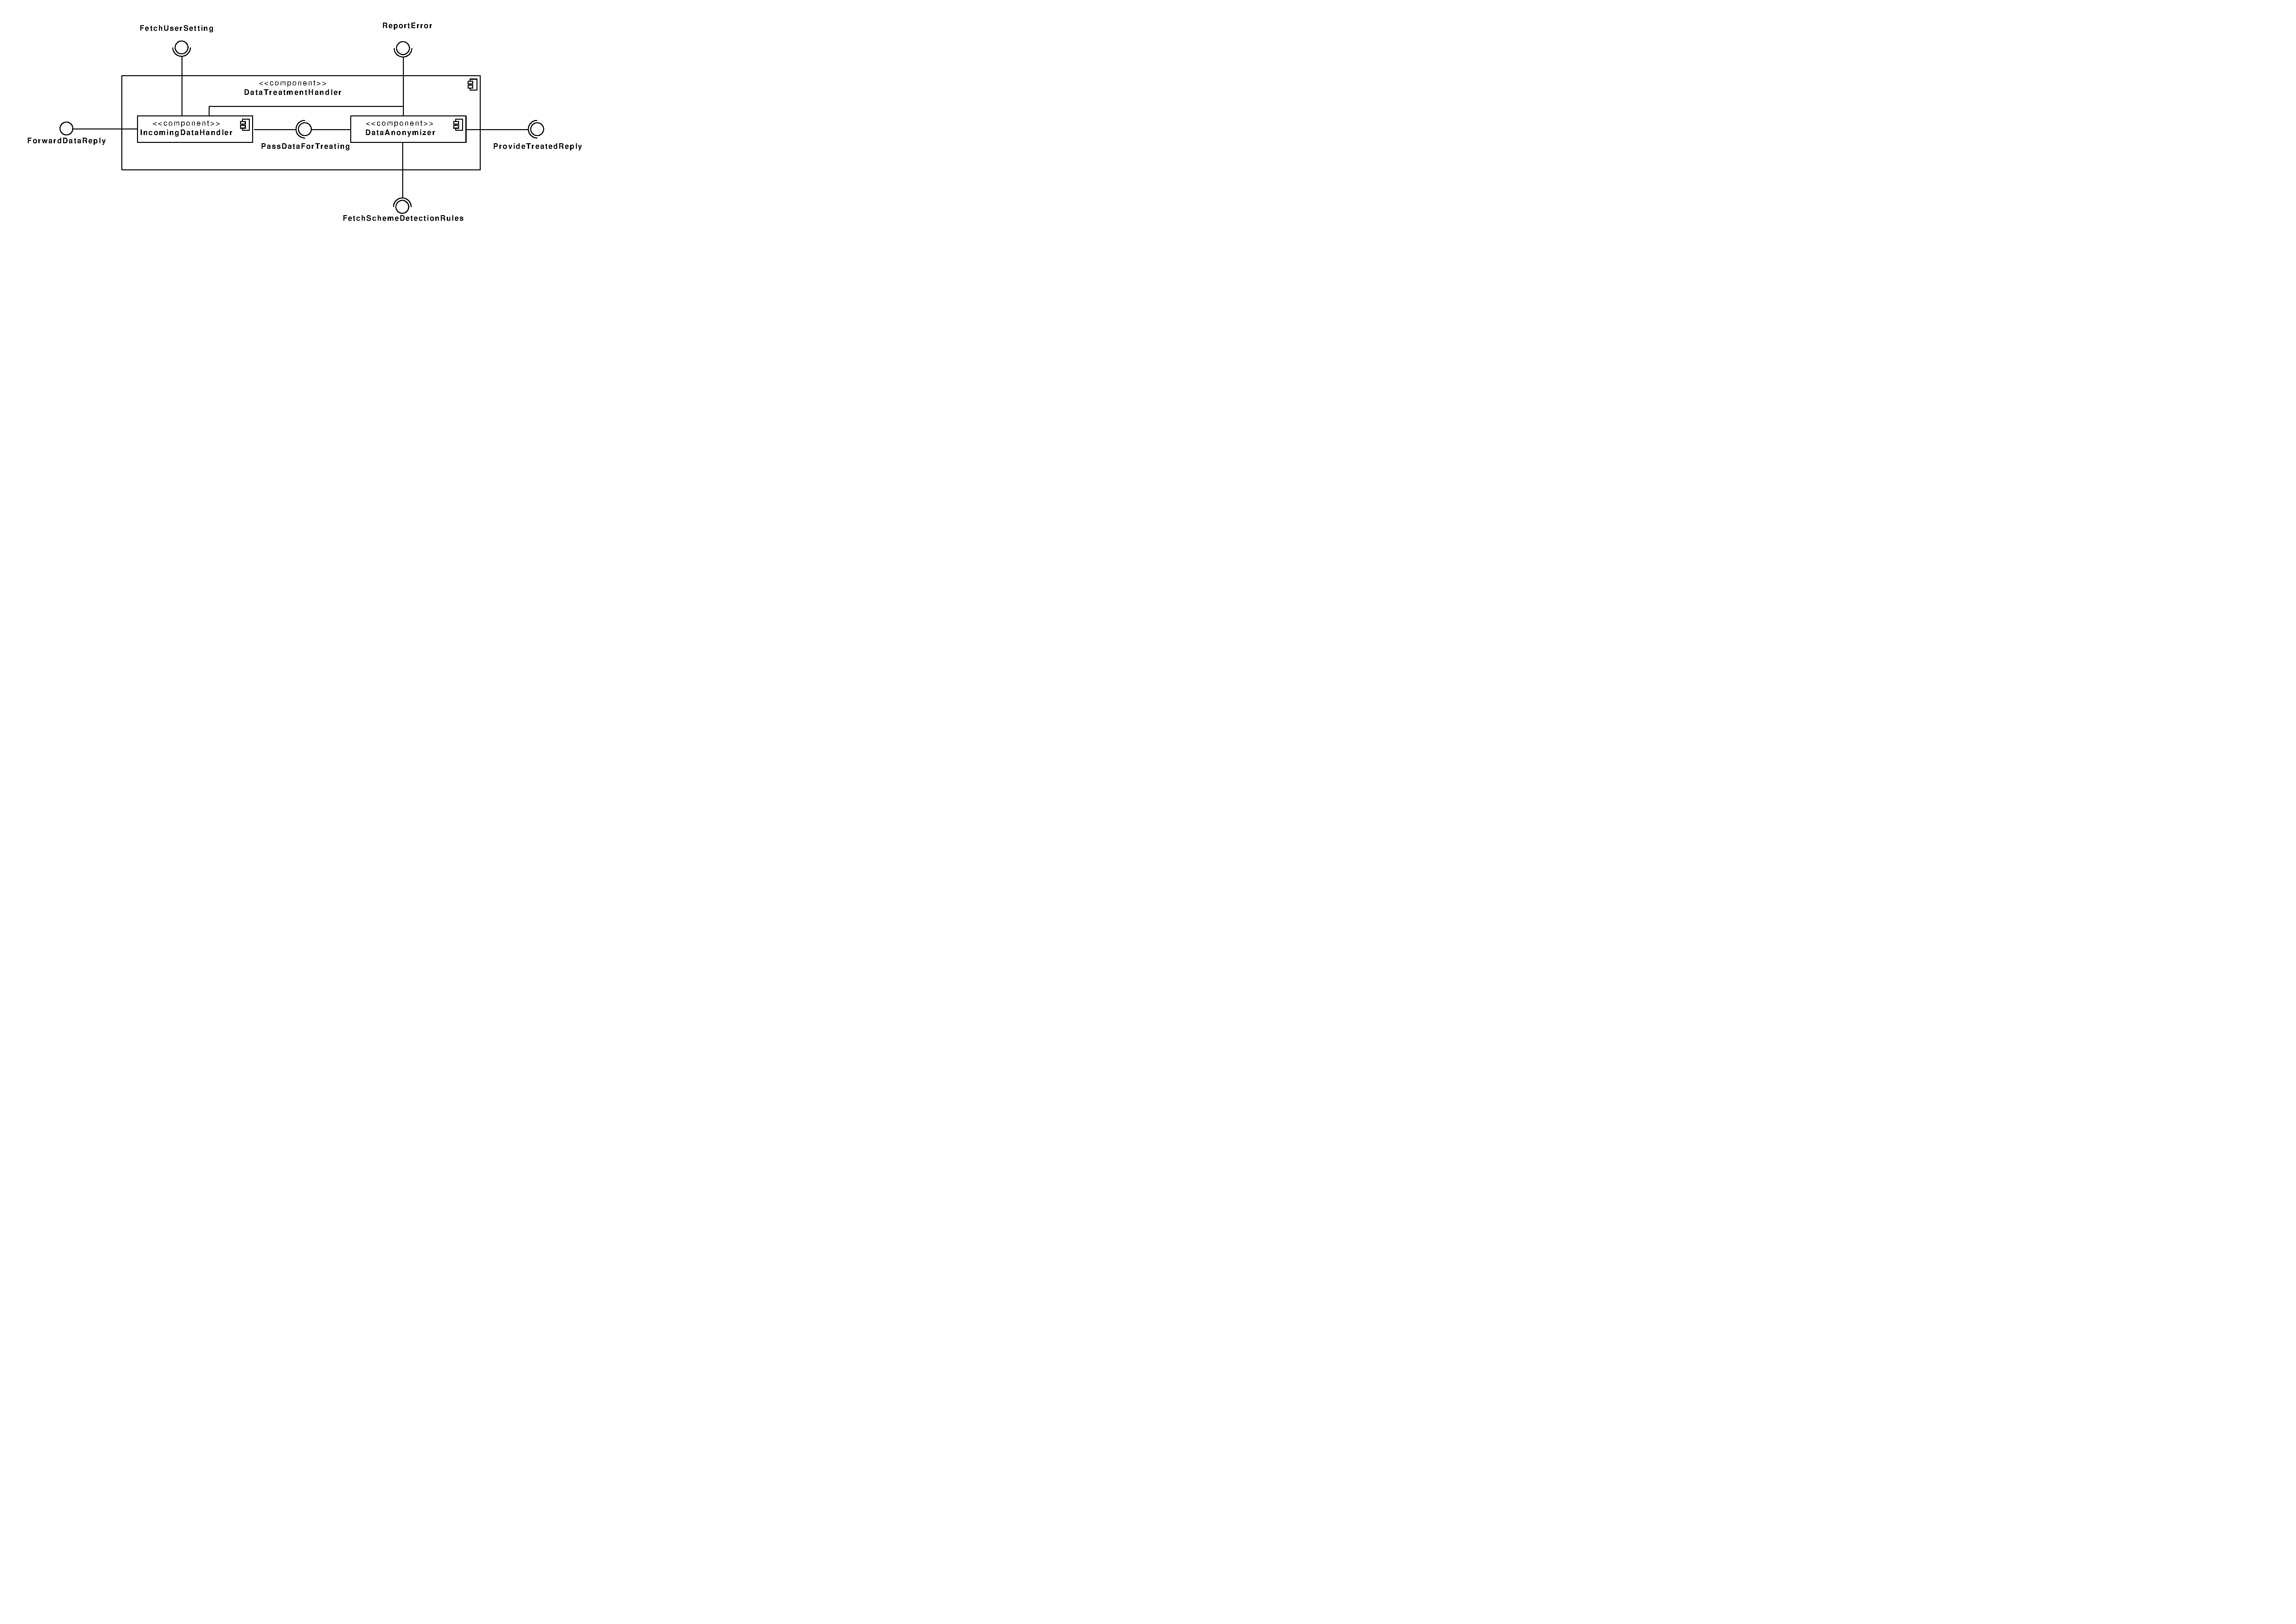
\includegraphics[width=\maxwidth{\textwidth}]{appendices/architecture/images/ComponentDiagram-DataTreatmentHandler-Component-Diagram.pdf}
  \caption[DataTreatmentHandler Component Diagram]{DataTreatmentHandler Component Diagram \label{diag:Component:DataTreatmentHandlerComponentDiagram}}
\end{figure}

%%% IncomingDataHandler Component Diagram (679.0x374.0)

\begin{figure}[!htp]
  \centering
  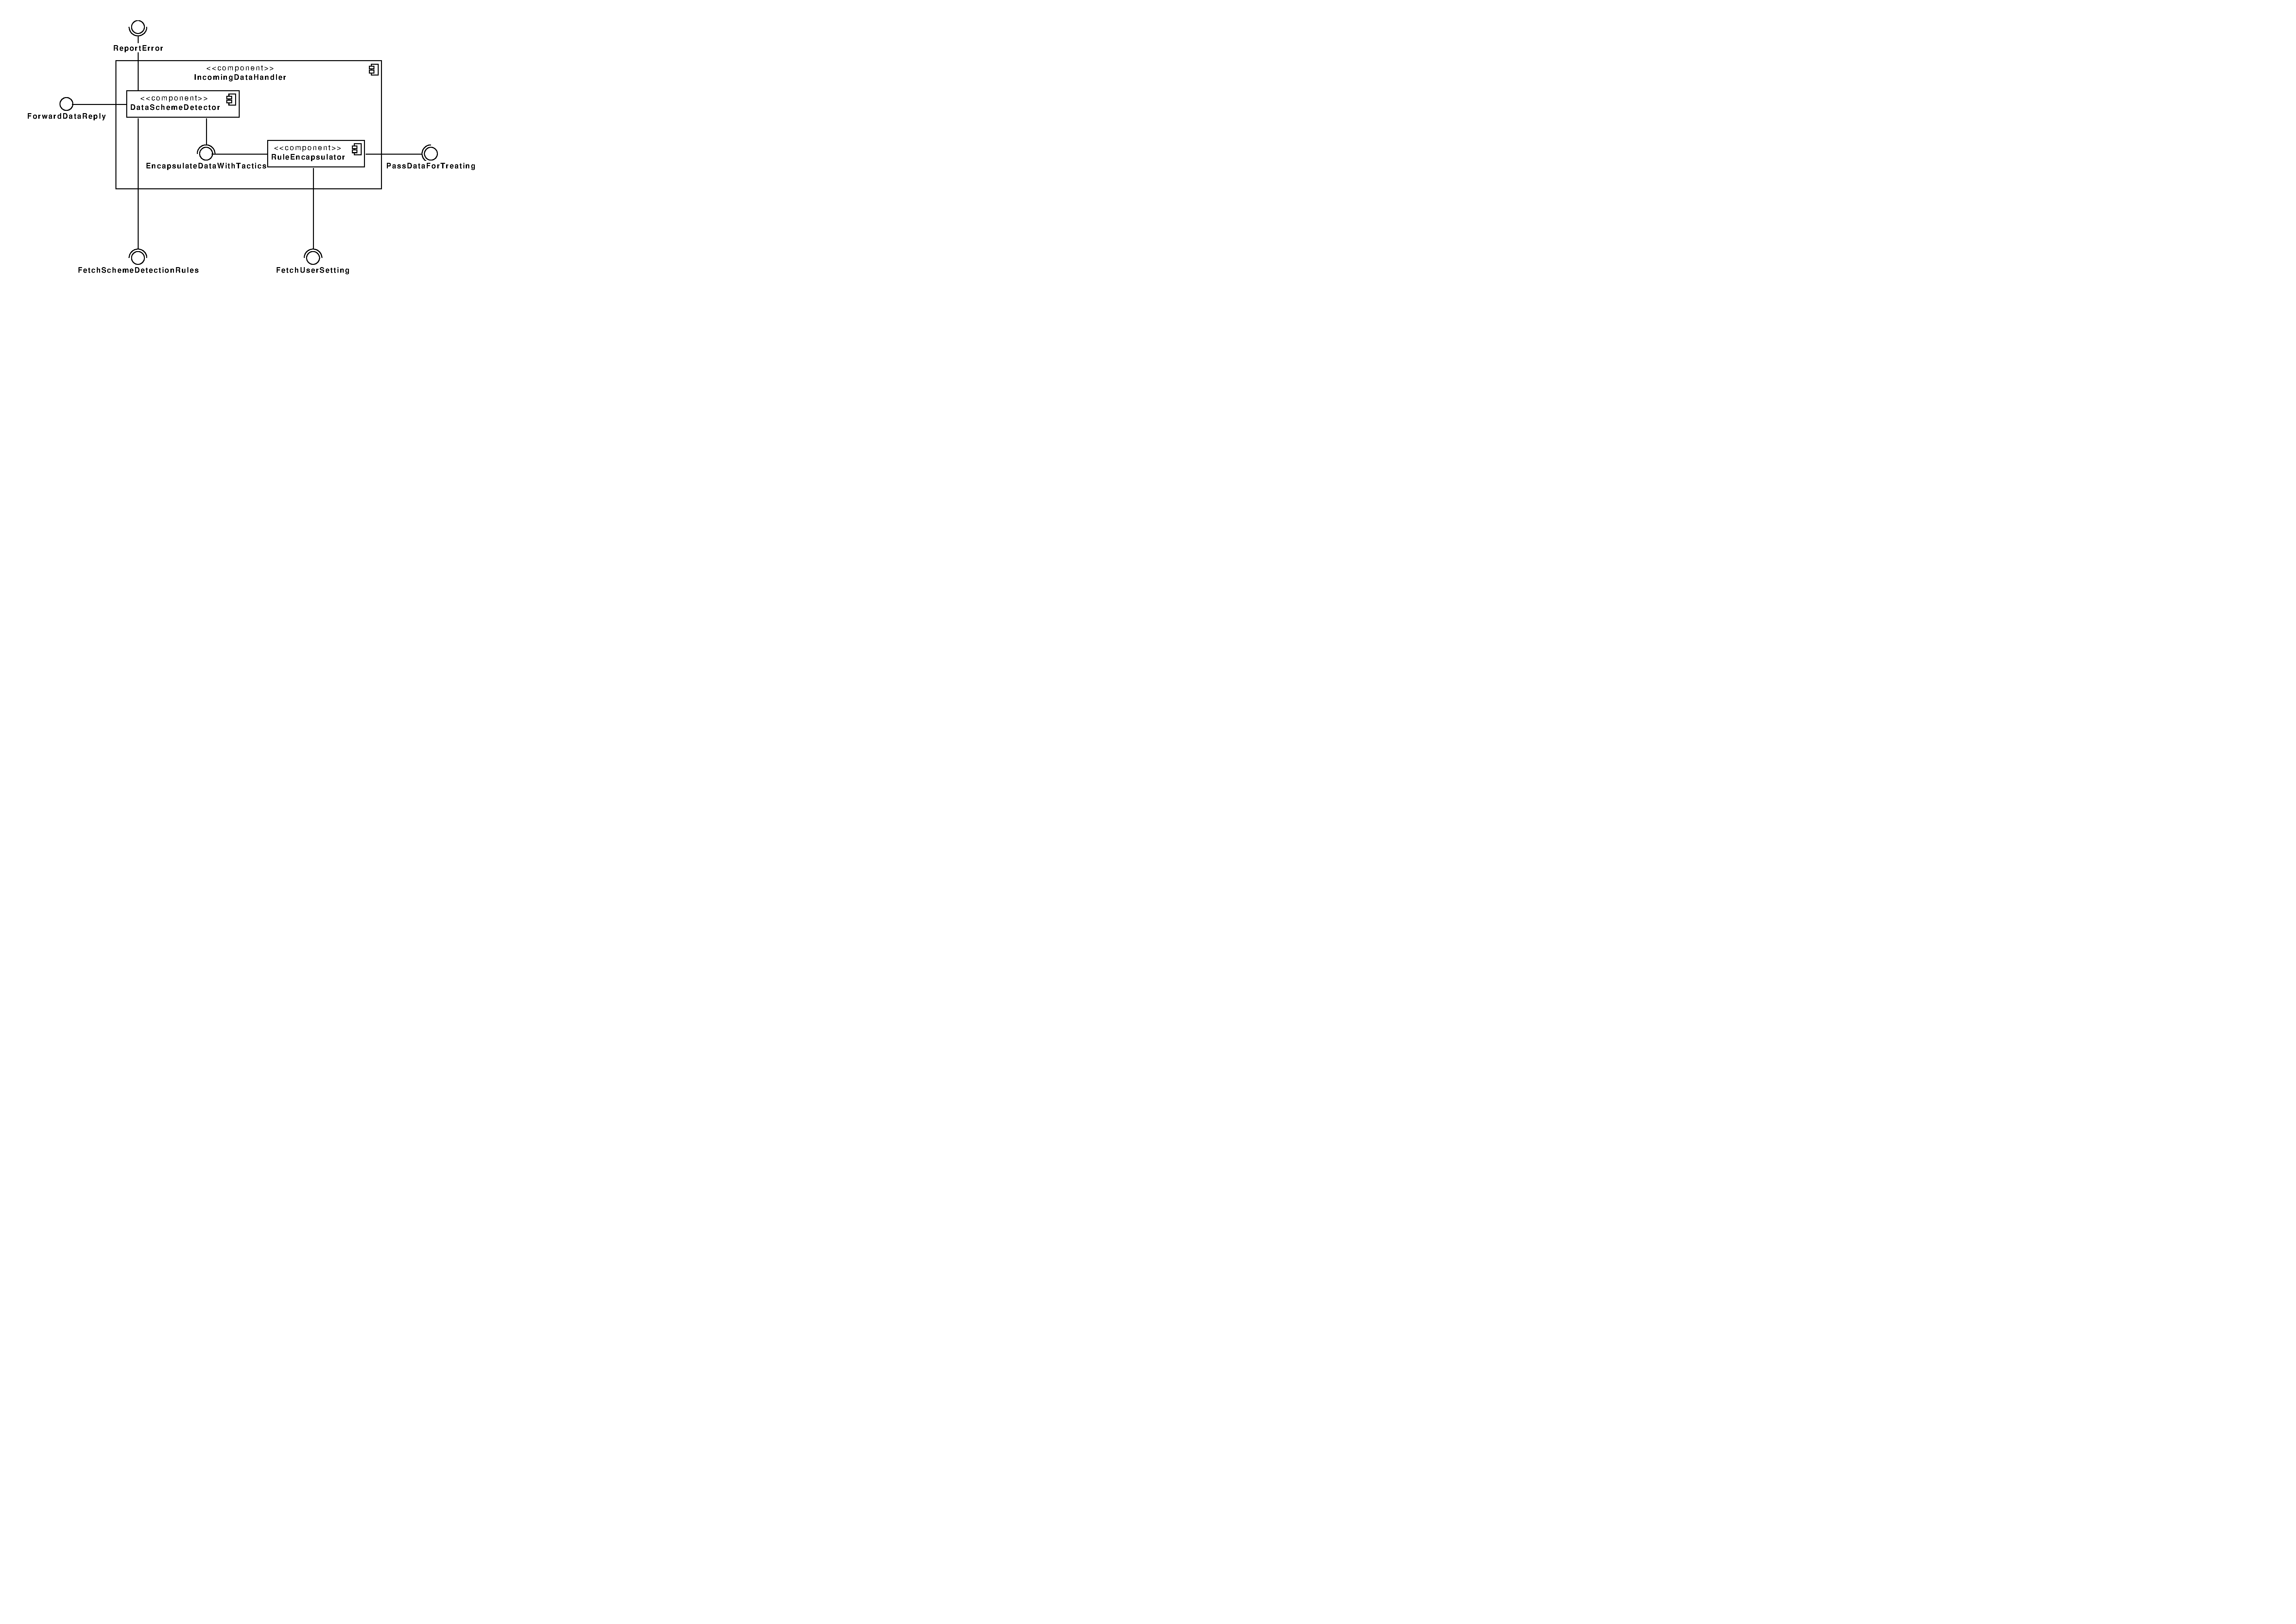
\includegraphics[width=\maxwidth{\textwidth}]{appendices/architecture/images/ComponentDiagram-IncomingDataHandler-Component-Diagram.pdf}
  \caption[IncomingDataHandler Component Diagram]{IncomingDataHandler Component Diagram \label{diag:Component:IncomingDataHandlerComponentDiagram}}
\end{figure}

%%% OutgoingHTTPHandler Component Diagram (833.0x316.0)

\begin{figure}[!htp]
  \centering
  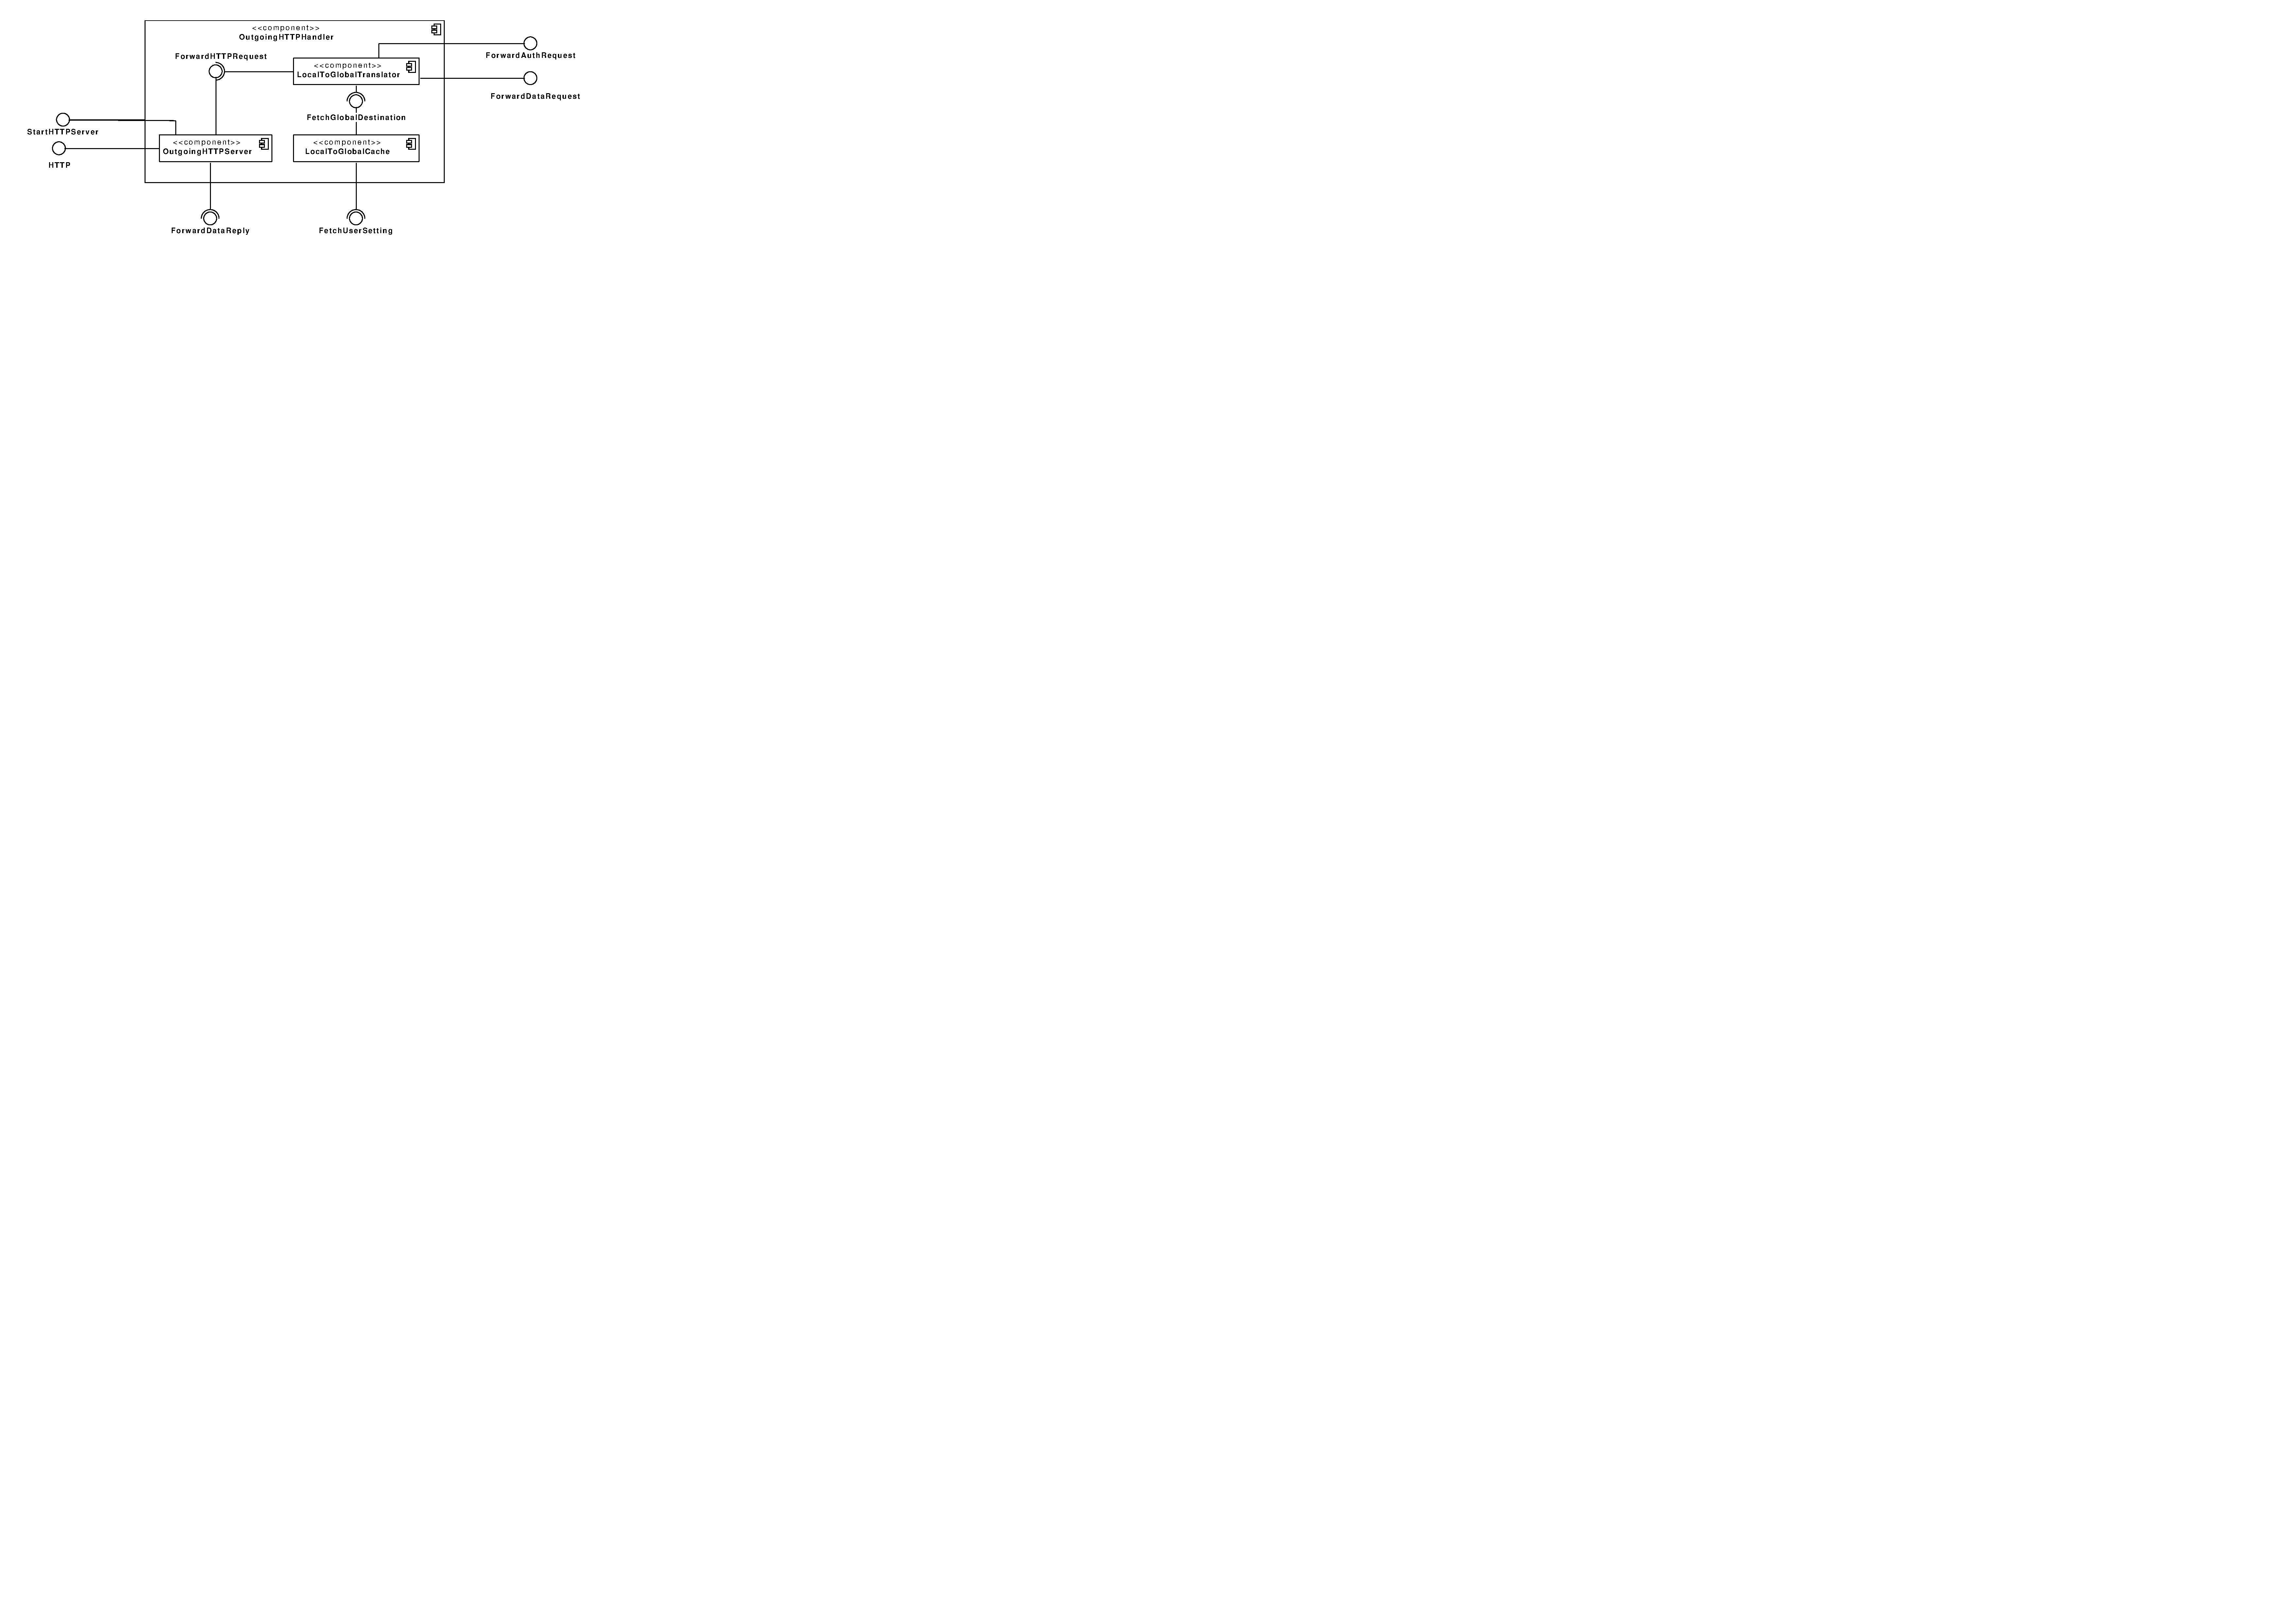
\includegraphics[width=\maxwidth{\textwidth}]{appendices/architecture/images/ComponentDiagram-OutgoingHTTPHandler-Component-Diagram.pdf}
  \caption[OutgoingHTTPHandler Component Diagram]{OutgoingHTTPHandler Component Diagram \label{diag:Component:OutgoingHTTPHandlerComponentDiagram}}
\end{figure}

%%% System Overview (927.0x393.0)

\begin{figure}[!htp]
  \centering
  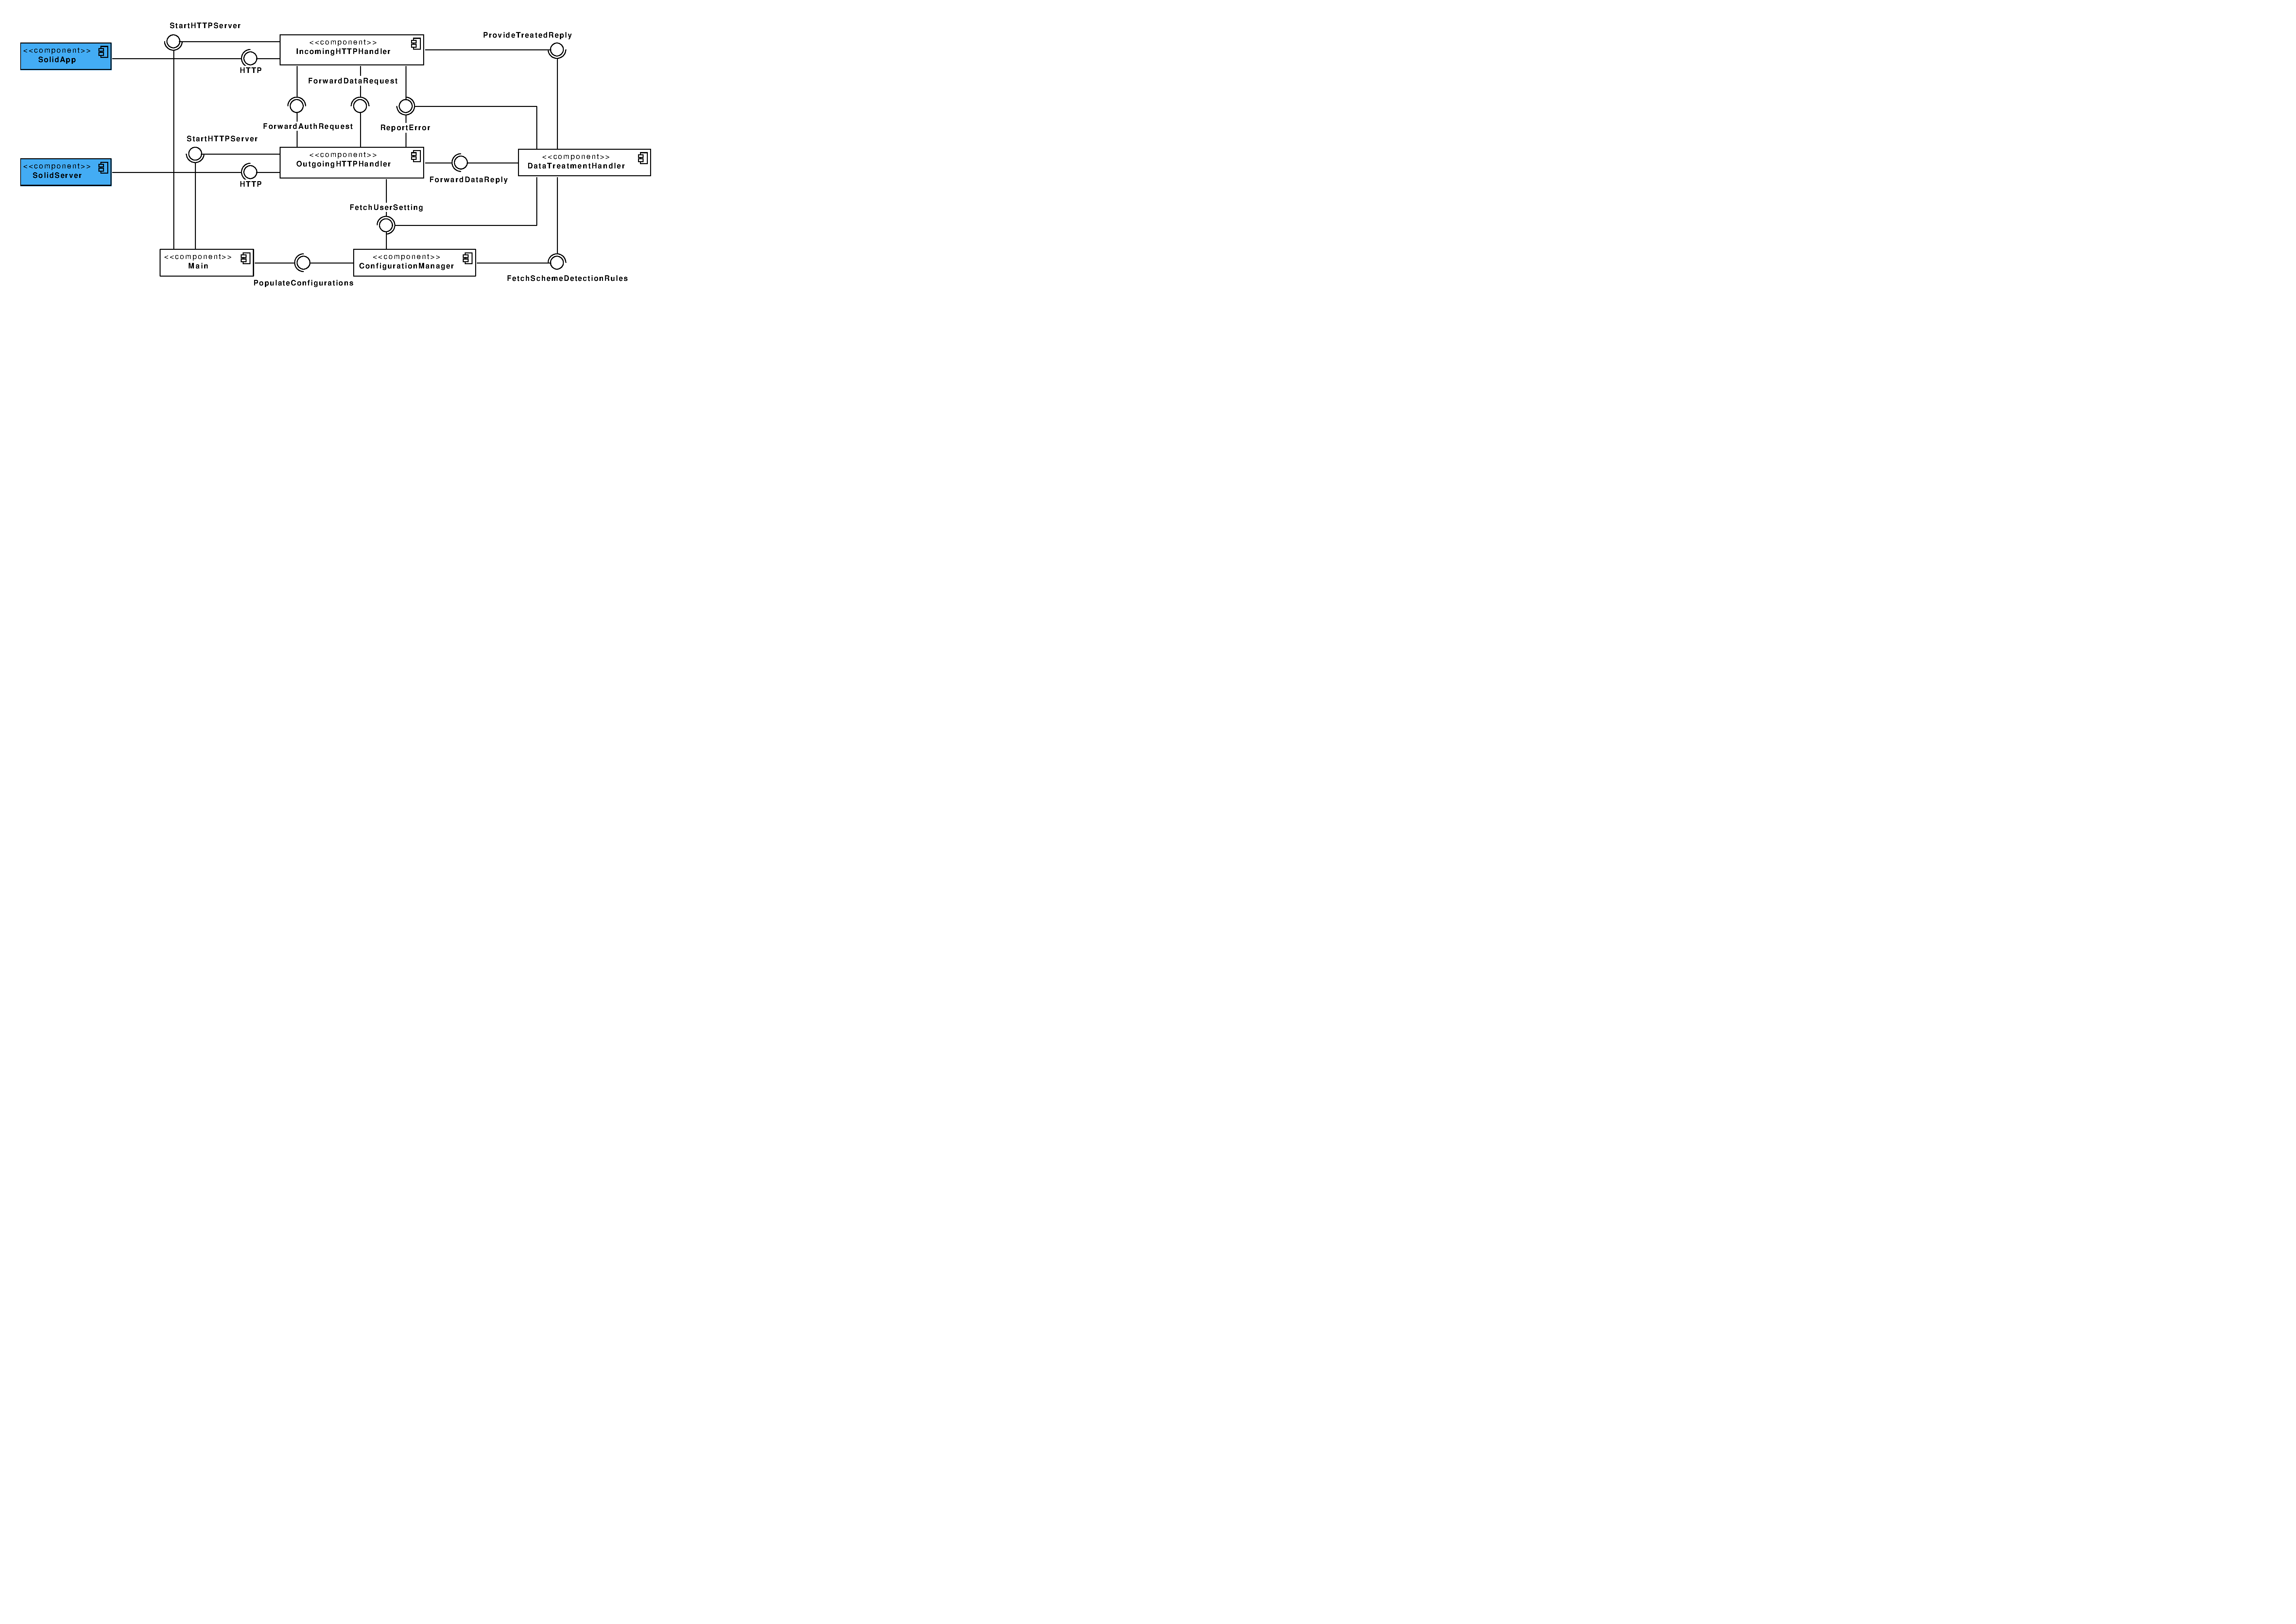
\includegraphics[width=\maxwidth{\textwidth}]{appendices/architecture/images/ComponentDiagram-System-Overview.pdf}
  \caption[System Overview]{System Overview \label{diag:Component:SystemOverview}}
\end{figure}



%%%%%%%%%%%%%%%%%%%%%%%%%%%%%%%%%%%%%%%%%%%%%%%%%%%%
%%% DEPLOYMENT
%%%%%%%%%%%%%%%%%%%%%%%%%%%%%%%%%%%%%%%%%%%%%%%%%%%%
\chapter{Deployment view (UML Deployment Diagram)}
\minilof{}




%%% Deployment Diagram (953.0x282.0)

\begin{figure}[!htp]
  \centering
  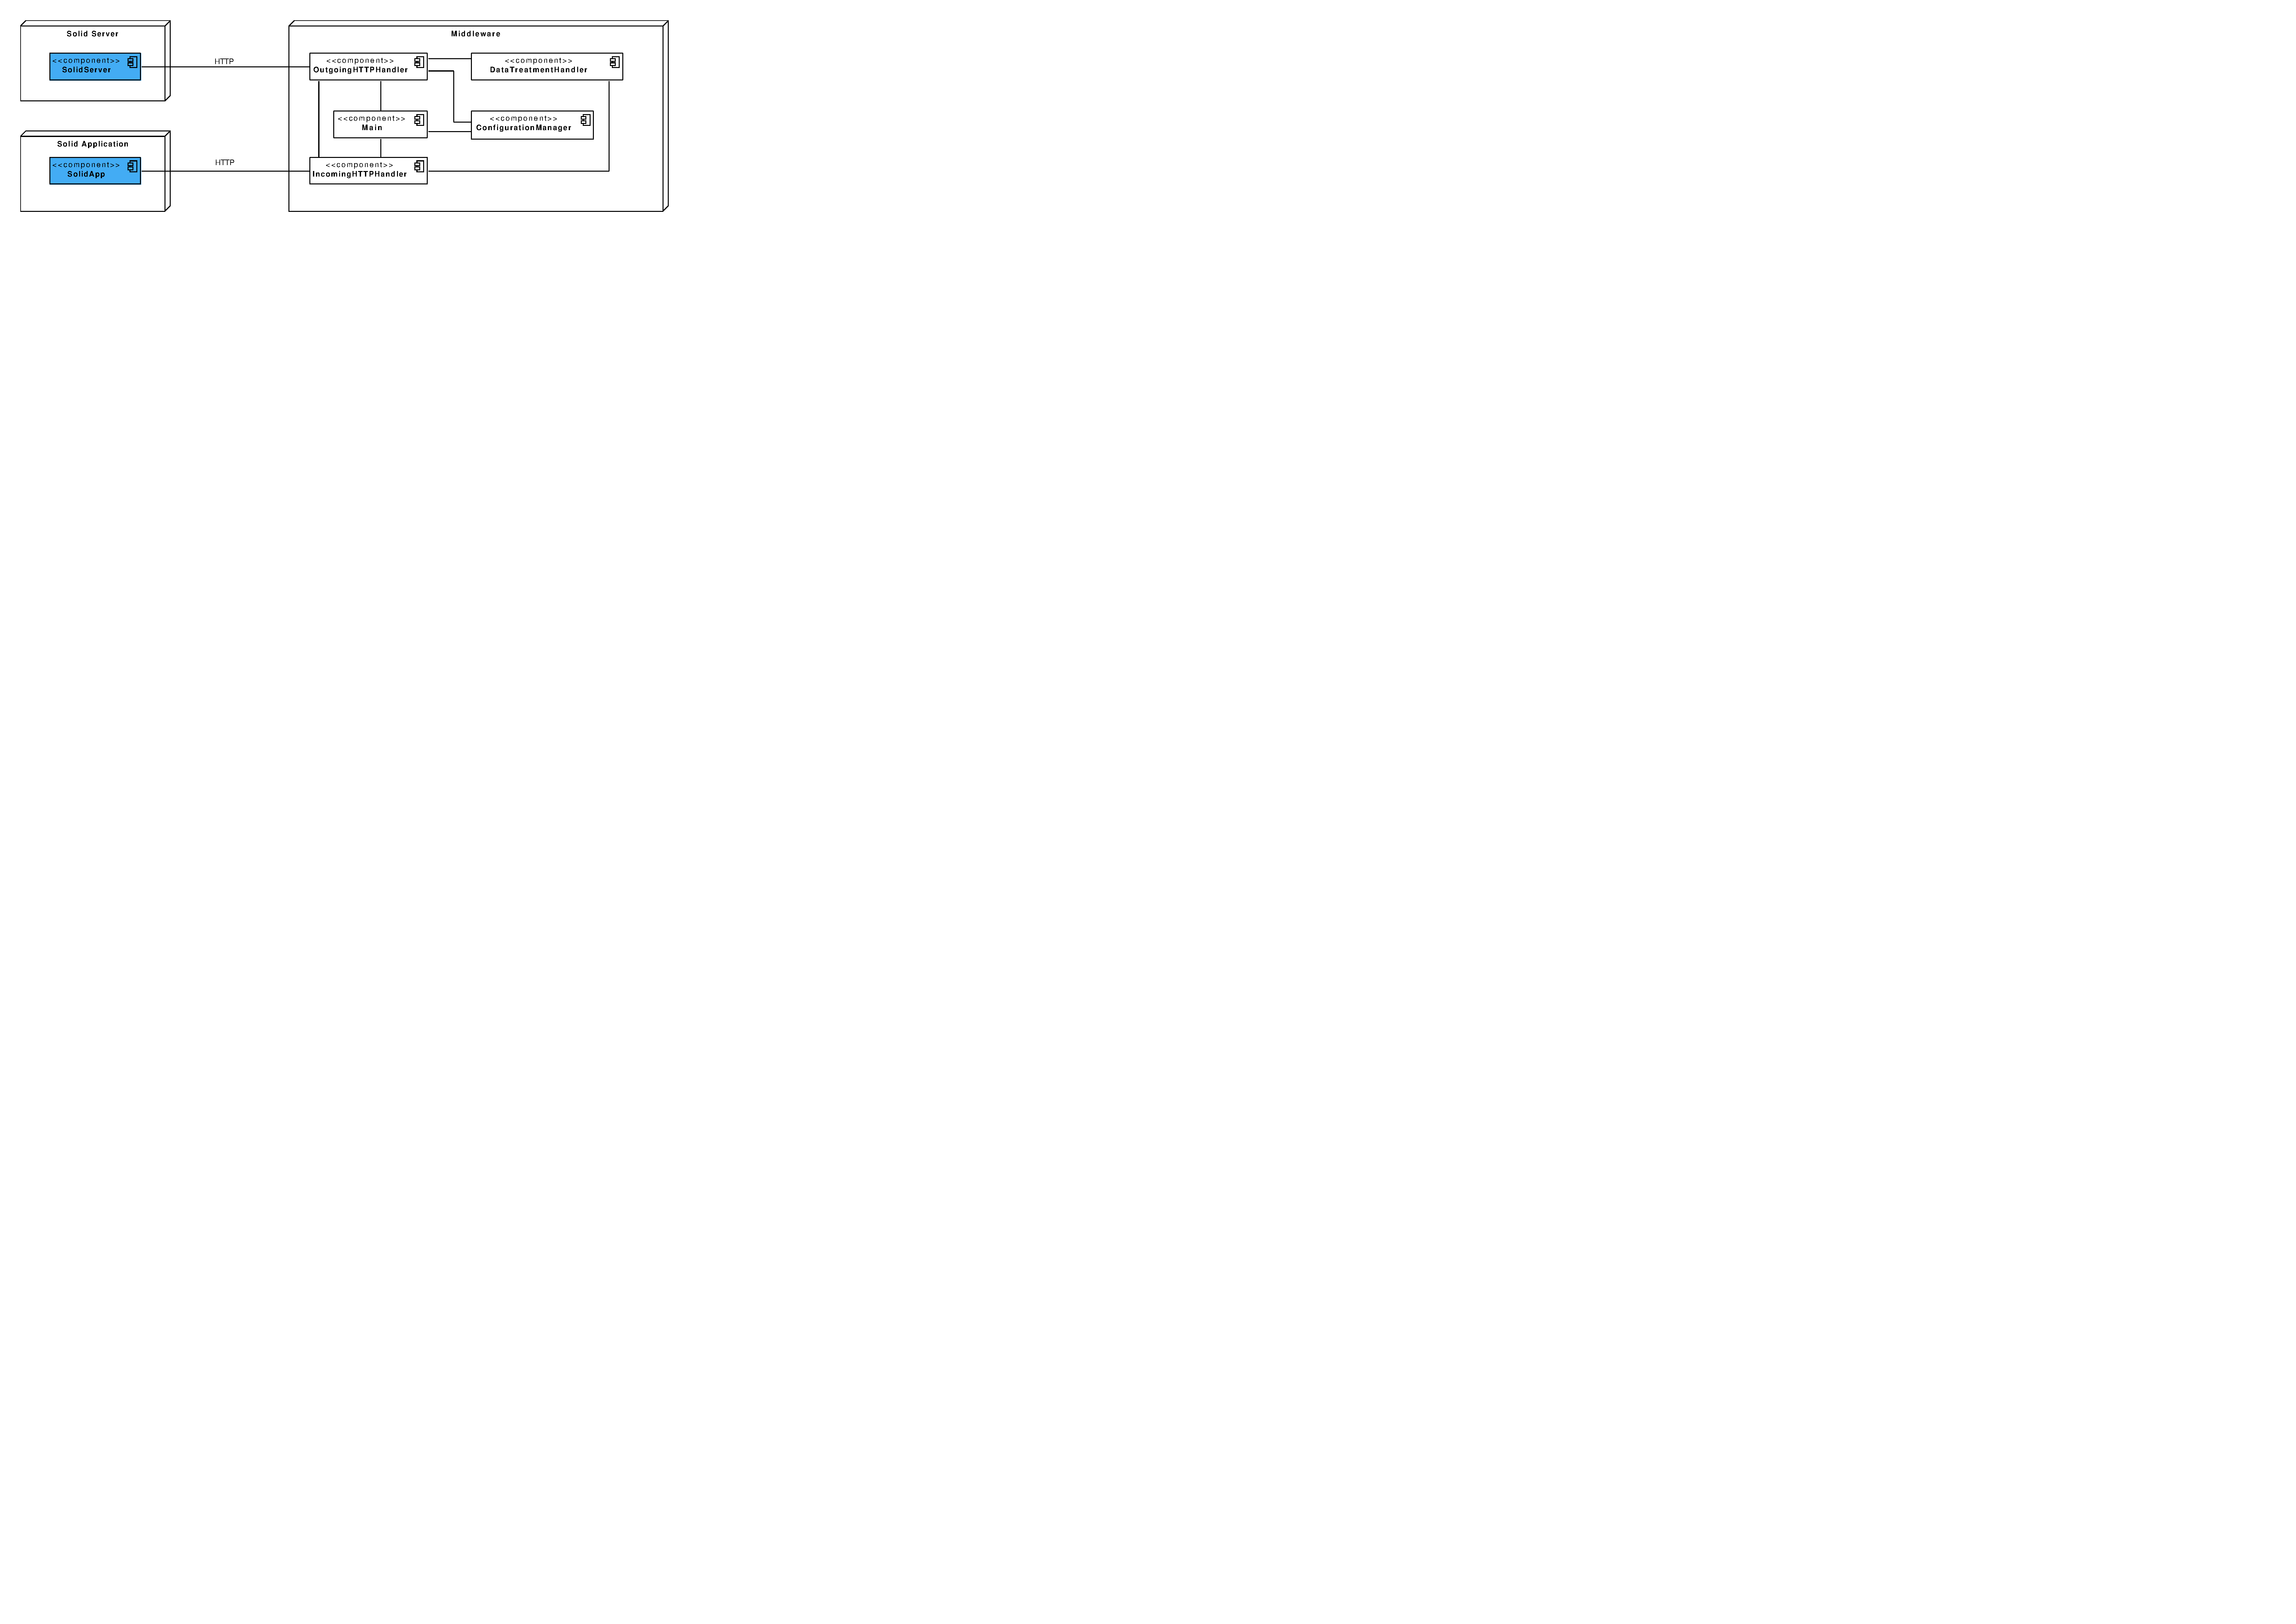
\includegraphics[width=\maxwidth{\textwidth}]{appendices/architecture/images/DeploymentDiagram-Deployment-Diagram.pdf}
  \caption[Deployment Diagram]{Deployment Diagram \label{diag:Deployment:DeploymentDiagram}}
\end{figure}



%%%%%%%%%%%%%%%%%%%%%%%%%%%%%%%%%%%%%%%%%%%%%%%%%%%%
%%% SEQUENCE
%%%%%%%%%%%%%%%%%%%%%%%%%%%%%%%%%%%%%%%%%%%%%%%%%%%%
\chapter{Process View (UML Sequence Diagram)}
\minilof{}


%%% Data flow (1305.0x406.0)

\begin{figure}[!htp]
  \centering
  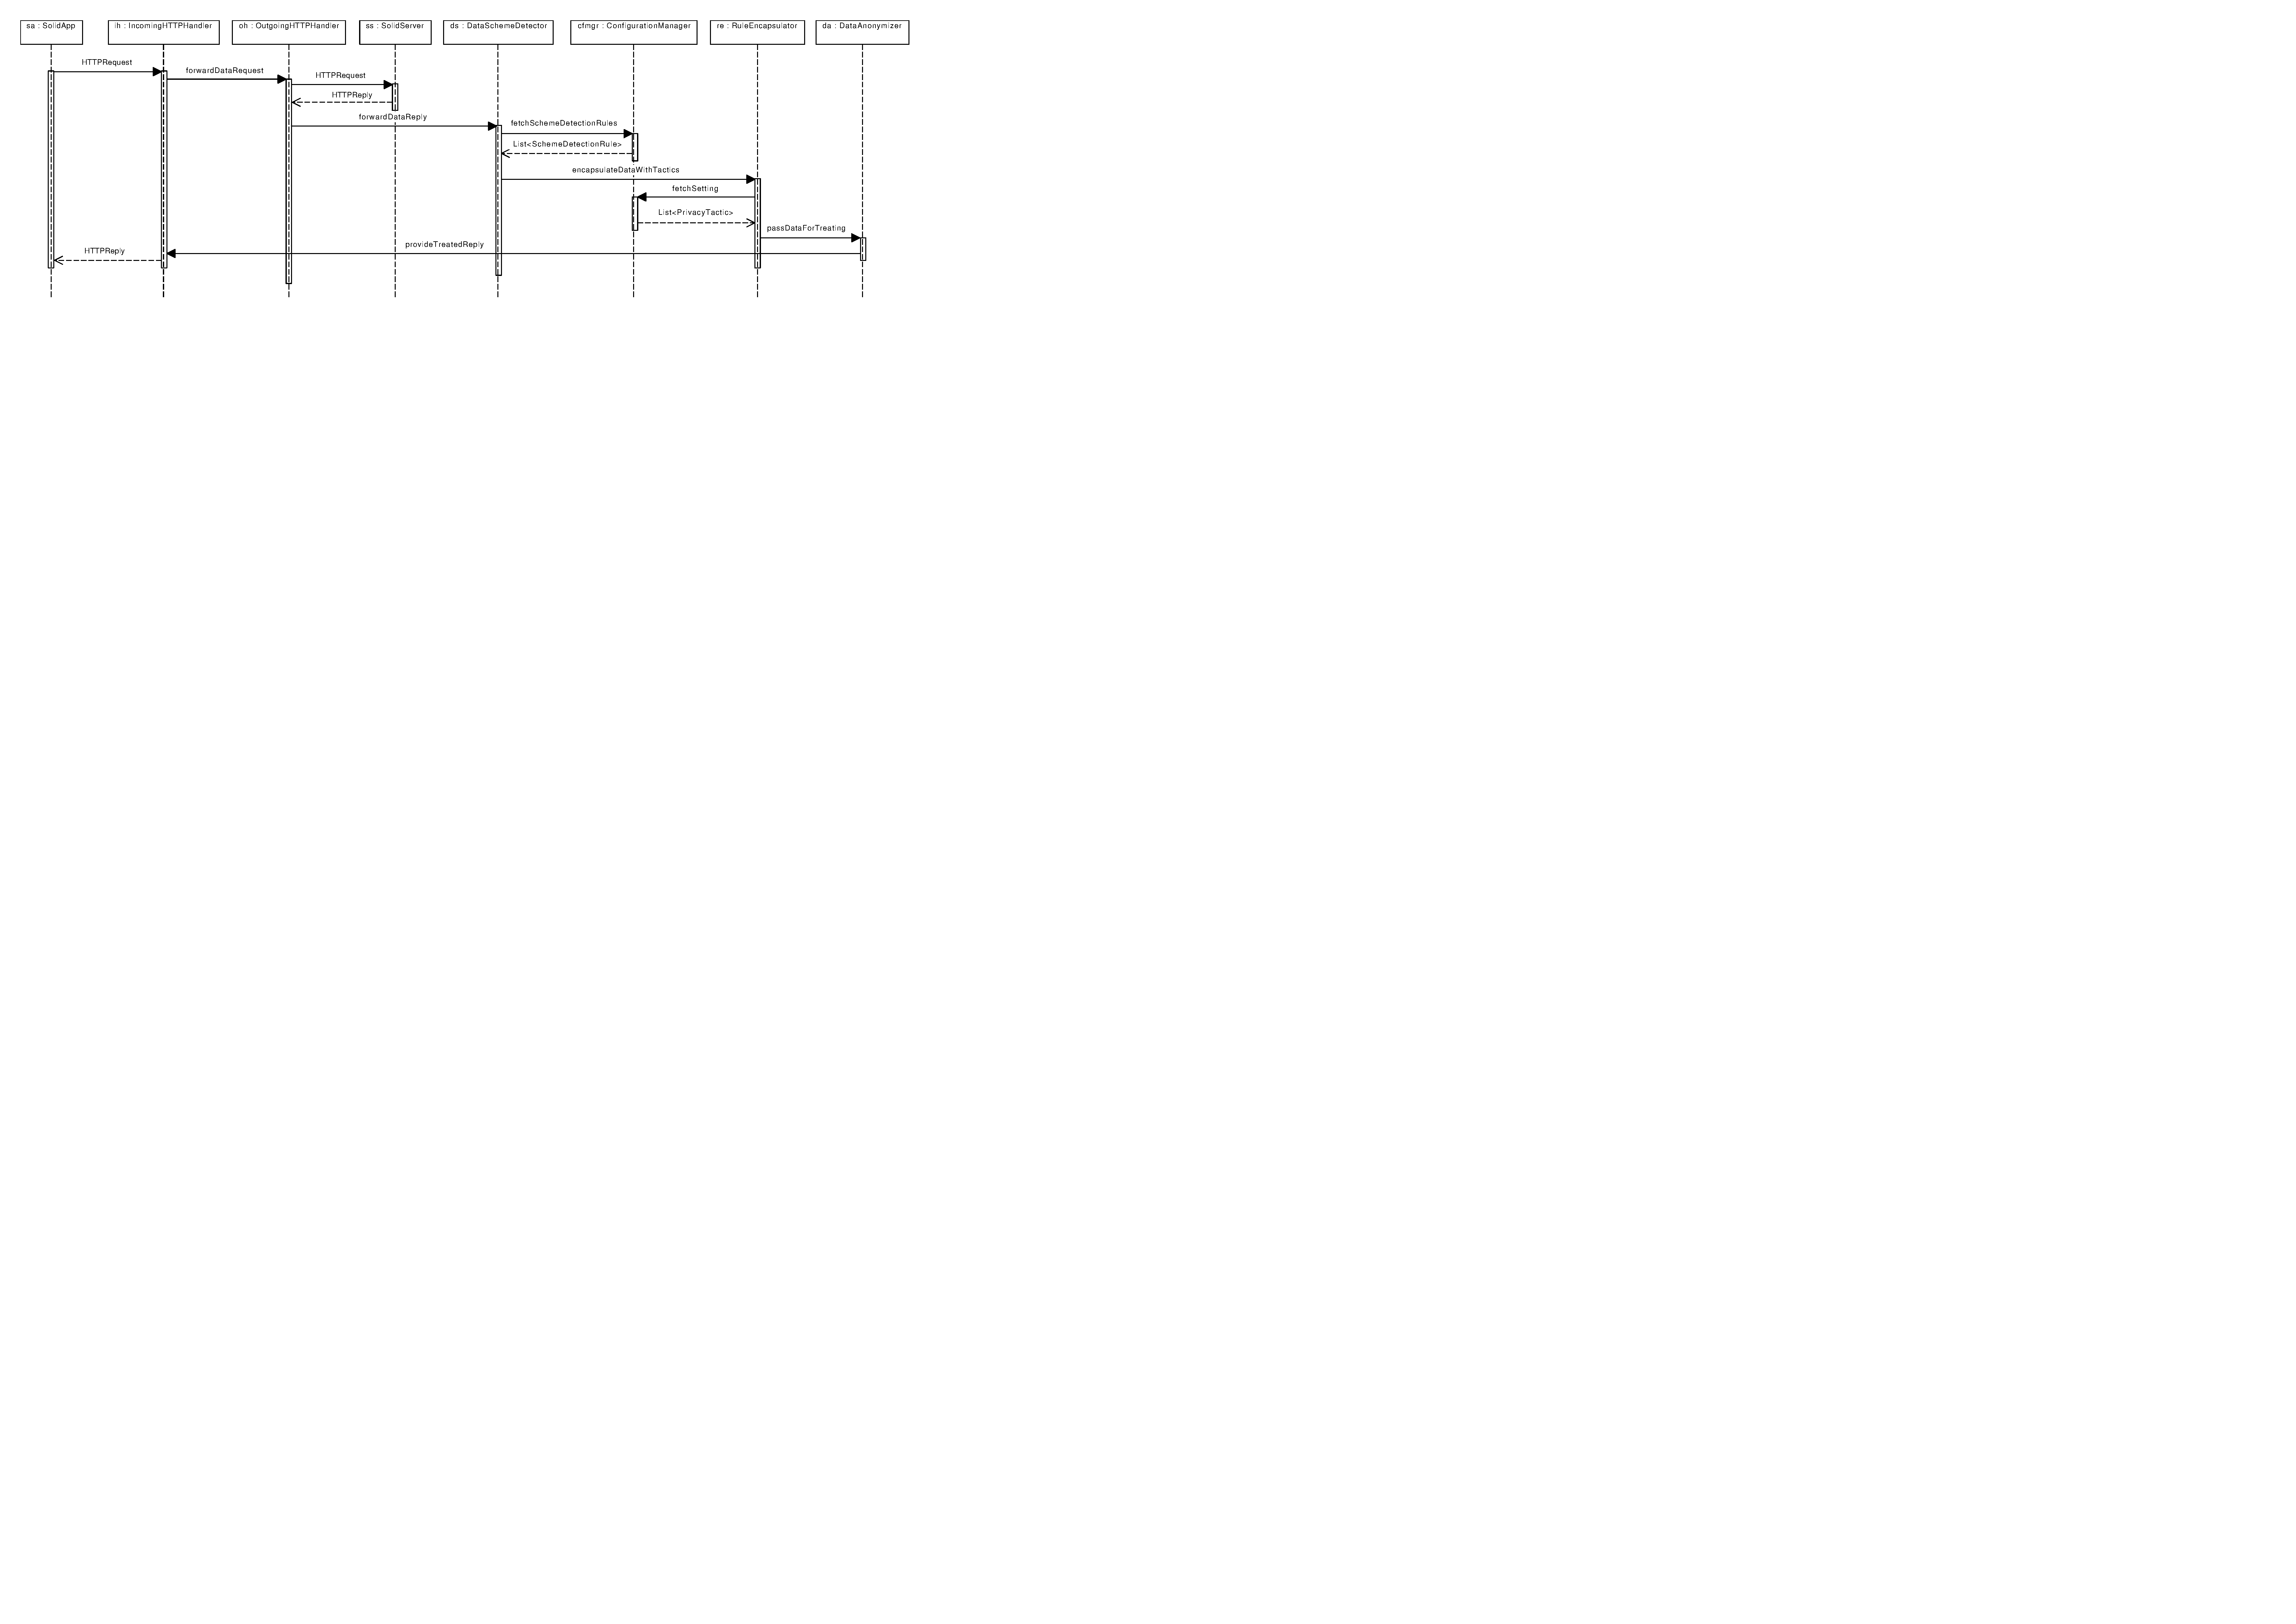
\includegraphics[width=\maxwidth{\textwidth}]{appendices/architecture/images/InteractionDiagram-Data-flow.pdf}
  \caption[Data flow]{Data flow \label{diag:Interaction:Dataflow}}
\end{figure}

%%%% element catalog, generated on Sun Nov 28 22:49:53 CET 2021

%%% WARNING %%%
%%% This file was automatically generated by SAPlugin,
%%% and will be overwritten next time.

\chapter{Element catalog}\label{sec:catalog}
% COMPONENTS
\section{Components}\label{sec:components}
\subsection{ConfigurationManager}\label{comp:ComponentsConfigurationManager}
	\begin{description}[noitemsep,nolistsep]
		\item[Responsibility:]~The \vpett{\nameref{comp:ComponentsConfigurationManager}} component is responsible for storing all configurable settings, such as:
* The URL of the user's pod to connect to
* The URL the middleware should be deployed to
* A list of supported data schemes, and for each data scheme the settings as to which privacy level maps to which transformations
* Which privacy level should be applied (either by default, or for specific data schemes)
		\item[Super-components:]~None
		\item[Sub-components:]~None
		\item[Provided interfaces:]~\iconprovided{}~\vpett{\nameref{int:InterfacesFetchSchemeDetectionRules}}, \iconprovided{}~\vpett{\nameref{int:InterfacesFetchUserSetting}}, \iconprovided{}~\vpett{\nameref{int:InterfacesPopulateConfigurations}}
		\item[Required interfaces:]~None
		\item[Deployed on:]~\faSquareO~\vpett{\nameref{node:DeploymentMiddleware}}
		\item[Visible on diagrams:]~\cref{diag:Component:SystemOverview,diag:Deployment:DeploymentDiagram,diag:Interaction:Dataflow}		
	\end{description}

\subsection{DataAnonymizer}\label{comp:ComponentsDataTreatmentHandlerDataAnonymizer}
	\begin{description}[noitemsep,nolistsep]
		\item[Responsibility:]~The \vpett{\nameref{comp:ComponentsDataTreatmentHandlerDataAnonymizer}} is the main component responsible for taking in raw data (of which the scheme has already been detected, and the tactics necessary to be performed have been added to the data). It then performs all the required tactics on the data, using different components based on the content-representation of the data.
When no scheme is detected, a "\ref{data:ExceptionsNoMatchingSchemeException}" is thrown.
		\item[Super-components:]~\iconcomponent{}~\vpett{\nameref{comp:ComponentsDataTreatmentHandler}}
		\item[Sub-components:]~\iconcomponent{}~\vpett{\nameref{comp:ComponentsDataTreatmentHandlerDataAnonymizerJSONTacticParser}}, \iconcomponent{}~\vpett{\nameref{comp:ComponentsDataTreatmentHandlerDataAnonymizerXMLTacticParser}}, \iconcomponent{}~\vpett{\nameref{comp:ComponentsDataTreatmentHandlerDataAnonymizerParserSelector}}
		\item[Provided interfaces:]~\iconprovided{}~\vpett{\nameref{int:InterfacesPassDataForTreating}}
		\item[Required interfaces:]~\iconrequired{}~\vpett{\nameref{int:InterfacesFetchSchemeDetectionRules}}, \iconrequired{}~\vpett{\nameref{int:InterfacesProvideTreatedReply}}, \iconrequired{}~\vpett{\nameref{int:InterfacesReportError}}
		\item[Deployed on:]~\faSquareO~\vpett{\nameref{node:DeploymentMiddleware}}
		\item[Visible on diagrams:]~\cref{diag:Component:DataAnonymizerComponentDiagram,diag:Component:DataTreatmentHandlerComponentDiagram,diag:Interaction:Dataflow}		
	\end{description}

\subsection{DataSchemeDetector}\label{comp:ComponentsDataTreatmentHandlerIncomingDataHandlerDataSchemeDetector}
	\begin{description}[noitemsep,nolistsep]
		\item[Responsibility:]~The \vpett{\nameref{comp:ComponentsDataTreatmentHandlerIncomingDataHandlerDataSchemeDetector}} is the component responsible for taking in raw data, and then (using a set of SchemeDetectionRules), determining which scheme the data uses.
		\item[Super-components:]~\iconcomponent{}~\vpett{\nameref{comp:ComponentsDataTreatmentHandlerIncomingDataHandler}} $\triangleright$ \iconcomponent{}~\vpett{\nameref{comp:ComponentsDataTreatmentHandler}}
		\item[Sub-components:]~None
		\item[Provided interfaces:]~\iconprovided{}~\vpett{\nameref{int:InterfacesForwardDataReply}}, \iconprovided{}~\vpett{\nameref{int:InterfacesPassDataForTreating}}
		\item[Required interfaces:]~\iconrequired{}~\vpett{\nameref{int:InterfacesEncapsulateDataWithTactics}}, \iconrequired{}~\vpett{\nameref{int:InterfacesFetchSchemeDetectionRules}}, \iconrequired{}~\vpett{\nameref{int:InterfacesReportError}}
		\item[Deployed on:]~\faSquareO~\vpett{\nameref{node:DeploymentMiddleware}}
		\item[Visible on diagrams:]~\cref{diag:Component:IncomingDataHandlerComponentDiagram,diag:Interaction:Dataflow}		
	\end{description}

\subsection{DataTreatmentHandler}\label{comp:ComponentsDataTreatmentHandler}
	\begin{description}[noitemsep,nolistsep]
		\item[Responsibility:]~The DataRequestHandler forms the bulk of the application logic: it takes the replied data from the \vpett{\nameref{comp:ComponentsOutgoingHTTPHandler}}, and passes it through the \vpett{\nameref{comp:ComponentsDataTreatmentHandlerDataAnonymizer}} to apply the right transformations, before going through the OutgoingDataHandler to detect possible errors and return the transformed data to the \vpett{\nameref{comp:ComponentsIncomingHTTPHandler}}.
		\item[Super-components:]~None
		\item[Sub-components:]~\iconcomponent{}~\vpett{\nameref{comp:ComponentsDataTreatmentHandlerIncomingDataHandler}}, \iconcomponent{}~\vpett{\nameref{comp:ComponentsDataTreatmentHandlerDataAnonymizer}}
		\item[Provided interfaces:]~\iconprovided{}~\vpett{\nameref{int:InterfacesForwardDataReply}}
		\item[Required interfaces:]~\iconrequired{}~\vpett{\nameref{int:InterfacesFetchSchemeDetectionRules}}, \iconrequired{}~\vpett{\nameref{int:InterfacesFetchUserSetting}}, \iconrequired{}~\vpett{\nameref{int:InterfacesProvideTreatedReply}}, \iconrequired{}~\vpett{\nameref{int:InterfacesReportError}}
		\item[Deployed on:]~\faSquareO~\vpett{\nameref{node:DeploymentMiddleware}}
		\item[Visible on diagrams:]~\cref{diag:Component:DataTreatmentHandlerComponentDiagram,diag:Component:SystemOverview,diag:Deployment:DeploymentDiagram}		
	\end{description}

\subsection{IncomingDataHandler}\label{comp:ComponentsDataTreatmentHandlerIncomingDataHandler}
	\begin{description}[noitemsep,nolistsep]
		\item[Responsibility:]~The \vpett{\nameref{comp:ComponentsDataTreatmentHandlerIncomingDataHandler}} receives the data that is passed on from the \vpett{\nameref{comp:ComponentsOutgoingHTTPHandler}}. It then detects the scheme of the data and fetches the correct TransfromationRules to be applied to this data, which is then passed on to the \vpett{\nameref{comp:ComponentsDataTreatmentHandlerDataAnonymizer}}.
		\item[Super-components:]~\iconcomponent{}~\vpett{\nameref{comp:ComponentsDataTreatmentHandler}}
		\item[Sub-components:]~\iconcomponent{}~\vpett{\nameref{comp:ComponentsDataTreatmentHandlerIncomingDataHandlerRuleEncapsulator}}, \iconcomponent{}~\vpett{\nameref{comp:ComponentsDataTreatmentHandlerIncomingDataHandlerDataSchemeDetector}}
		\item[Provided interfaces:]~\iconprovided{}~\vpett{\nameref{int:InterfacesForwardDataReply}}
		\item[Required interfaces:]~\iconrequired{}~\vpett{\nameref{int:InterfacesFetchSchemeDetectionRules}}, \iconrequired{}~\vpett{\nameref{int:InterfacesFetchUserSetting}}, \iconrequired{}~\vpett{\nameref{int:InterfacesPassDataForTreating}}, \iconrequired{}~\vpett{\nameref{int:InterfacesReportError}}
		\item[Deployed on:]~\faSquareO~\vpett{\nameref{node:DeploymentMiddleware}}
		\item[Visible on diagrams:]~\cref{diag:Component:DataTreatmentHandlerComponentDiagram,diag:Component:IncomingDataHandlerComponentDiagram}		
	\end{description}

\subsection{IncomingHTTPHandler}\label{comp:ComponentsIncomingHTTPHandler}
	\begin{description}[noitemsep,nolistsep]
		\item[Responsibility:]~This component is responsible for handling incoming HTTP requests (i.e., from the Solid application, which sends a request to the solid server).
		\item[Super-components:]~None
		\item[Sub-components:]~None
		\item[Provided interfaces:]~\iconprovided{}~\vpett{\nameref{int:InterfacesHTTP}}, \iconprovided{}~\vpett{\nameref{int:InterfacesProvideTreatedReply}}, \iconprovided{}~\vpett{\nameref{int:InterfacesReportError}}, \iconprovided{}~\vpett{\nameref{int:InterfacesStartHTTPServer}}
		\item[Required interfaces:]~\iconrequired{}~\vpett{\nameref{int:InterfacesForwardAuthRequest}}, \iconrequired{}~\vpett{\nameref{int:InterfacesForwardDataRequest}}
		\item[Deployed on:]~\faSquareO~\vpett{\nameref{node:DeploymentMiddleware}}
		\item[Visible on diagrams:]~\cref{diag:Component:SystemOverview,diag:Deployment:DeploymentDiagram,diag:Interaction:Dataflow}		
	\end{description}

\subsection{JSONTacticParser}\label{comp:ComponentsDataTreatmentHandlerDataAnonymizerJSONTacticParser}
	\begin{description}[noitemsep,nolistsep]
		\item[Responsibility:]~The \vpett{\nameref{comp:ComponentsDataTreatmentHandlerDataAnonymizerJSONTacticParser}} is responsible for taking in the raw data (in JSON) and applying the encapsulated PrivacyTactics to the data before providing the treated data to the \vpett{\nameref{comp:ComponentsIncomingHTTPHandler}}.
		\item[Super-components:]~\iconcomponent{}~\vpett{\nameref{comp:ComponentsDataTreatmentHandlerDataAnonymizer}} $\triangleright$ \iconcomponent{}~\vpett{\nameref{comp:ComponentsDataTreatmentHandler}}
		\item[Sub-components:]~None
		\item[Provided interfaces:]~\iconprovided{}~\vpett{\nameref{int:InterfacesPassDataForTreating}}
		\item[Required interfaces:]~\iconrequired{}~\vpett{\nameref{int:InterfacesProvideTreatedReply}}
		\item[Deployed on:]~\faSquareO~\vpett{\nameref{node:DeploymentMiddleware}}
		\item[Visible on diagrams:]~\cref{diag:Component:DataAnonymizerComponentDiagram}		
	\end{description}

\subsection{LocalToGlobalCache}\label{comp:ComponentsOutgoingHTTPHandlerLocalToGlobalCache}
	\begin{description}[noitemsep,nolistsep]
		\item[Responsibility:]~The \vpett{\nameref{comp:ComponentsOutgoingHTTPHandlerLocalToGlobalCache}} is a cache that stores translations from the local to global destination. If no entry is found in the cache, the appropriate global destination is fetched from the \vpett{\nameref{comp:ComponentsConfigurationManager}}.
		\item[Super-components:]~\iconcomponent{}~\vpett{\nameref{comp:ComponentsOutgoingHTTPHandler}}
		\item[Sub-components:]~None
		\item[Provided interfaces:]~\iconprovided{}~\vpett{\nameref{int:InterfacesFetchGlobalDestination}}
		\item[Required interfaces:]~\iconrequired{}~\vpett{\nameref{int:InterfacesFetchUserSetting}}
		\item[Deployed on:]~\faSquareO~\vpett{\nameref{node:DeploymentMiddleware}}
		\item[Visible on diagrams:]~\cref{diag:Component:OutgoingHTTPHandlerComponentDiagram}		
	\end{description}

\subsection{LocalToGlobalTranslator}\label{comp:ComponentsOutgoingHTTPHandlerLocalToGlobalTranslator}
	\begin{description}[noitemsep,nolistsep]
		\item[Responsibility:]~The \vpett{\nameref{comp:ComponentsOutgoingHTTPHandlerLocalToGlobalTranslator}} is responsible for modifying an auth or data request, so that it can go to the \vpett{\nameref{comp:ComponentsOutgoingHTTPHandlerOutgoingHTTPServer}}. Concretely, when a request arrives, the URI still contains the domain of the middleware. This should be replaced with the domain of the \vpett{\nameref{comp:ComponentsSolidServer}}. The FetchGlobalDestination is used fetch the global destination.
		\item[Super-components:]~\iconcomponent{}~\vpett{\nameref{comp:ComponentsOutgoingHTTPHandler}}
		\item[Sub-components:]~None
		\item[Provided interfaces:]~\iconprovided{}~\vpett{\nameref{int:InterfacesForwardAuthRequest}}, \iconprovided{}~\vpett{\nameref{int:InterfacesForwardDataRequest}}
		\item[Required interfaces:]~\iconrequired{}~\vpett{\nameref{int:InterfacesFetchGlobalDestination}}, \iconrequired{}~\vpett{\nameref{int:InterfacesForwardHTTPRequest}}
		\item[Deployed on:]~\faSquareO~\vpett{\nameref{node:DeploymentMiddleware}}
		\item[Visible on diagrams:]~\cref{diag:Component:OutgoingHTTPHandlerComponentDiagram}		
	\end{description}

\subsection{Main}\label{comp:ComponentsMain}
	\begin{description}[noitemsep,nolistsep]
		\item[Responsibility:]~The entry-point of the program. This component is responsible for starting up the HTTP Server, and reading/parsing all configuration files (user settings and supported plugins/schemes).
		\item[Super-components:]~None
		\item[Sub-components:]~None
		\item[Provided interfaces:]~None
		\item[Required interfaces:]~\iconrequired{}~\vpett{\nameref{int:InterfacesPopulateConfigurations}}, \iconrequired{}~\vpett{\nameref{int:InterfacesStartHTTPServer}}
		\item[Deployed on:]~\faSquareO~\vpett{\nameref{node:DeploymentMiddleware}}
		\item[Visible on diagrams:]~\cref{diag:Component:SystemOverview,diag:Deployment:DeploymentDiagram}		
	\end{description}

\subsection{OutgoingHTTPHandler}\label{comp:ComponentsOutgoingHTTPHandler}
	\begin{description}[noitemsep,nolistsep]
		\item[Responsibility:]~The OutgoingHTTP is an HTTP client that is responsible for communication with the Solid server. When a data request is forwarded, it will send this request to the solid server, waiting for a reply, and then passing on the received data.
		\item[Super-components:]~None
		\item[Sub-components:]~\iconcomponent{}~\vpett{\nameref{comp:ComponentsOutgoingHTTPHandlerLocalToGlobalTranslator}}, \iconcomponent{}~\vpett{\nameref{comp:ComponentsOutgoingHTTPHandlerLocalToGlobalCache}}, \iconcomponent{}~\vpett{\nameref{comp:ComponentsOutgoingHTTPHandlerOutgoingHTTPServer}}
		\item[Provided interfaces:]~\iconprovided{}~\vpett{\nameref{int:InterfacesForwardAuthRequest}}, \iconprovided{}~\vpett{\nameref{int:InterfacesForwardDataRequest}}, \iconprovided{}~\vpett{\nameref{int:InterfacesHTTP}}, \iconprovided{}~\vpett{\nameref{int:InterfacesStartHTTPServer}}
		\item[Required interfaces:]~\iconrequired{}~\vpett{\nameref{int:InterfacesFetchUserSetting}}, \iconrequired{}~\vpett{\nameref{int:InterfacesForwardDataReply}}, \iconrequired{}~\vpett{\nameref{int:InterfacesReportError}}
		\item[Deployed on:]~\faSquareO~\vpett{\nameref{node:DeploymentMiddleware}}
		\item[Visible on diagrams:]~\cref{diag:Component:OutgoingHTTPHandlerComponentDiagram,diag:Component:SystemOverview,diag:Deployment:DeploymentDiagram,diag:Interaction:Dataflow}		
	\end{description}

\subsection{OutgoingHTTPServer}\label{comp:ComponentsOutgoingHTTPHandlerOutgoingHTTPServer}
	\begin{description}[noitemsep,nolistsep]
		\item[Responsibility:]~The \vpett{\nameref{comp:ComponentsOutgoingHTTPHandlerOutgoingHTTPServer}} is an HTTP Server responsible for communication with the \vpett{\nameref{comp:ComponentsSolidServer}}.
		\item[Super-components:]~\iconcomponent{}~\vpett{\nameref{comp:ComponentsOutgoingHTTPHandler}}
		\item[Sub-components:]~None
		\item[Provided interfaces:]~\iconprovided{}~\vpett{\nameref{int:InterfacesForwardHTTPRequest}}, \iconprovided{}~\vpett{\nameref{int:InterfacesHTTP}}, \iconprovided{}~\vpett{\nameref{int:InterfacesStartHTTPServer}}
		\item[Required interfaces:]~\iconrequired{}~\vpett{\nameref{int:InterfacesForwardDataReply}}
		\item[Deployed on:]~\faSquareO~\vpett{\nameref{node:DeploymentMiddleware}}
		\item[Visible on diagrams:]~\cref{diag:Component:OutgoingHTTPHandlerComponentDiagram}		
	\end{description}

\subsection{ParserSelector}\label{comp:ComponentsDataTreatmentHandlerDataAnonymizerParserSelector}
	\begin{description}[noitemsep,nolistsep]
		\item[Responsibility:]~The \vpett{\nameref{comp:ComponentsDataTreatmentHandlerDataAnonymizerParserSelector}} component is responsible for forwarding the data it receives to the correct TacticParser, based on the content-representation of the data.
		\item[Super-components:]~\iconcomponent{}~\vpett{\nameref{comp:ComponentsDataTreatmentHandlerDataAnonymizer}} $\triangleright$ \iconcomponent{}~\vpett{\nameref{comp:ComponentsDataTreatmentHandler}}
		\item[Sub-components:]~None
		\item[Provided interfaces:]~\iconprovided{}~\vpett{\nameref{int:InterfacesPassDataForTreating}}
		\item[Required interfaces:]~\iconrequired{}~\vpett{\nameref{int:InterfacesPassDataForTreating}}
		\item[Deployed on:]~\faSquareO~\vpett{\nameref{node:DeploymentMiddleware}}
		\item[Visible on diagrams:]~\cref{diag:Component:DataAnonymizerComponentDiagram}		
	\end{description}

\subsection{RuleEncapsulator}\label{comp:ComponentsDataTreatmentHandlerIncomingDataHandlerRuleEncapsulator}
	\begin{description}[noitemsep,nolistsep]
		\item[Responsibility:]~The \vpett{\nameref{comp:ComponentsDataTreatmentHandlerIncomingDataHandlerRuleEncapsulator}} is responsible for asking the \vpett{\nameref{comp:ComponentsConfigurationManager}} which privacy level corresponds to the given DataType. Then, it asks the \vpett{\nameref{comp:ComponentsConfigurationManager}} for a List of PrivacyTactics, which specify how the given data should be treated. Finally, an encapsulation datatype is constructed that contains all necessary information for the correct TacticParser to complete its work.
		\item[Super-components:]~\iconcomponent{}~\vpett{\nameref{comp:ComponentsDataTreatmentHandlerIncomingDataHandler}} $\triangleright$ \iconcomponent{}~\vpett{\nameref{comp:ComponentsDataTreatmentHandler}}
		\item[Sub-components:]~None
		\item[Provided interfaces:]~\iconprovided{}~\vpett{\nameref{int:InterfacesEncapsulateDataWithTactics}}
		\item[Required interfaces:]~\iconrequired{}~\vpett{\nameref{int:InterfacesFetchUserSetting}}, \iconrequired{}~\vpett{\nameref{int:InterfacesPassDataForTreating}}
		\item[Deployed on:]~\faSquareO~\vpett{\nameref{node:DeploymentMiddleware}}
		\item[Visible on diagrams:]~\cref{diag:Component:IncomingDataHandlerComponentDiagram,diag:Interaction:Dataflow}		
	\end{description}

\subsection{SolidApp}\label{comp:ComponentsSolidApp}
	\begin{description}[noitemsep,nolistsep]
		\item[Responsibility:]~This component represents the Solid Application the user wishes to connect to the middleware. It will send requests to the middleware, which will be forwarded to the Solid Server. When the server replies, the data is parsed, and a reply is sent to the application.
		\item[Super-components:]~None
		\item[Sub-components:]~None
		\item[Provided interfaces:]~None
		\item[Required interfaces:]~\iconrequired{}~\vpett{\nameref{int:InterfacesHTTP}}
		\item[Deployed on:]~\faSquareO~\vpett{\nameref{node:DeploymentSolidApplication}}
		\item[Visible on diagrams:]~\cref{diag:Component:SystemOverview,diag:Deployment:DeploymentDiagram,diag:Interaction:Dataflow}		
	\end{description}

\subsection{SolidServer}\label{comp:ComponentsSolidServer}
	\begin{description}[noitemsep,nolistsep]
		\item[Responsibility:]~This component represents the Solid server where the user's pod is stored. A reference to its URI is kept in the configuration file, which is loaded by the \vpett{\nameref{comp:ComponentsConfigurationManager}}. The middleware will connect to this server to fetch data, before processing it.
		\item[Super-components:]~None
		\item[Sub-components:]~None
		\item[Provided interfaces:]~None
		\item[Required interfaces:]~\iconrequired{}~\vpett{\nameref{int:InterfacesHTTP}}
		\item[Deployed on:]~\faSquareO~\vpett{\nameref{node:DeploymentSolidServer}}
		\item[Visible on diagrams:]~\cref{diag:Component:SystemOverview,diag:Deployment:DeploymentDiagram,diag:Interaction:Dataflow}		
	\end{description}

\subsection{XMLTacticParser}\label{comp:ComponentsDataTreatmentHandlerDataAnonymizerXMLTacticParser}
	\begin{description}[noitemsep,nolistsep]
		\item[Responsibility:]~The \vpett{\nameref{comp:ComponentsDataTreatmentHandlerDataAnonymizerXMLTacticParser}} is responsible for taking in the raw data (in XML) and applying the encapsulated PrivacyTactics to the data before providing the treated data to the \vpett{\nameref{comp:ComponentsIncomingHTTPHandler}}.
		\item[Super-components:]~\iconcomponent{}~\vpett{\nameref{comp:ComponentsDataTreatmentHandlerDataAnonymizer}} $\triangleright$ \iconcomponent{}~\vpett{\nameref{comp:ComponentsDataTreatmentHandler}}
		\item[Sub-components:]~None
		\item[Provided interfaces:]~\iconprovided{}~\vpett{\nameref{int:InterfacesPassDataForTreating}}
		\item[Required interfaces:]~\iconrequired{}~\vpett{\nameref{int:InterfacesProvideTreatedReply}}
		\item[Deployed on:]~\faSquareO~\vpett{\nameref{node:DeploymentMiddleware}}
		\item[Visible on diagrams:]~\cref{diag:Component:DataAnonymizerComponentDiagram}		
	\end{description}


% END COMPONENTS

% MODULES
% no modules
% END MODULES

% INTERFACES
\section{Interfaces} \label{sec:interfaces}
  %%%%%%%% EncapsulateDataWithTactics
  \subsection{EncapsulateDataWithTactics}\label{int:InterfacesEncapsulateDataWithTactics}
    \begin{description}[noitemsep,nolistsep]
      \item[Provided by:] \iconcomponent{}~\vpett{\nameref{comp:ComponentsDataTreatmentHandlerIncomingDataHandlerRuleEncapsulator}}
      \item[Required by:] \iconcomponent{}~\vpett{\nameref{comp:ComponentsDataTreatmentHandlerIncomingDataHandlerDataSchemeDetector}} 
           \item[Description]: This interface provides a method for the \vpett{\nameref{comp:ComponentsDataTreatmentHandlerIncomingDataHandlerDataSchemeDetector}} to pass its data, which now includes the detected DataScheme, to the \vpett{\nameref{comp:ComponentsDataTreatmentHandlerIncomingDataHandlerRuleEncapsulator}} which will encapsulate the PrivacyTactics that must be performed.
      \item[Operations:] ~
    \begin{itemize}[noitemsep,nolistsep,leftmargin=-.25cm]
      \item \textsf{void passToEncapsulate(\ref{data:DatatypesTreatableData} data, List\textless{}\ref{data:DatatypesPrivacyTactic}\textgreater{} tactics)}
        \begin{itemize}[noitemsep,nolistsep]
           \item Effect: This function takes the list of privacy tactics to be performed, and the data on which they should be performed, and passes it on to the \vpett{\nameref{comp:ComponentsDataTreatmentHandlerIncomingDataHandlerRuleEncapsulator}}. 
           \item Sequence Diagrams: None
        \end{itemize}
    \end{itemize}
      \item[Diagrams:] \cref{diag:Component:IncomingDataHandlerComponentDiagram}
    \end{description}

  %%%%%%%% FetchGlobalDestination
  \subsection{FetchGlobalDestination}\label{int:InterfacesFetchGlobalDestination}
    \begin{description}[noitemsep,nolistsep]
      \item[Provided by:] \iconcomponent{}~\vpett{\nameref{comp:ComponentsOutgoingHTTPHandlerLocalToGlobalCache}}
      \item[Required by:] \iconcomponent{}~\vpett{\nameref{comp:ComponentsOutgoingHTTPHandlerLocalToGlobalTranslator}} 
      \item[Operations:] ~
% no operations
      \item[Diagrams:] \cref{diag:Component:OutgoingHTTPHandlerComponentDiagram}
    \end{description}

  %%%%%%%% FetchSchemeDetectionRules
  \subsection{FetchSchemeDetectionRules}\label{int:InterfacesFetchSchemeDetectionRules}
    \begin{description}[noitemsep,nolistsep]
      \item[Provided by:] \iconcomponent{}~\vpett{\nameref{comp:ComponentsConfigurationManager}}
      \item[Required by:] \iconcomponent{}~\vpett{\nameref{comp:ComponentsDataTreatmentHandlerDataAnonymizer}}, \iconcomponent{}~\vpett{\nameref{comp:ComponentsDataTreatmentHandlerIncomingDataHandlerDataSchemeDetector}}, \iconcomponent{}~\vpett{\nameref{comp:ComponentsDataTreatmentHandler}}, \iconcomponent{}~\vpett{\nameref{comp:ComponentsDataTreatmentHandlerIncomingDataHandler}} 
           \item[Description]: This interface provides a method to retrieve a List<\ref{data:DatatypesSchemeDetectionRule}>, which are used to identify the resulting data scheme.
      \item[Operations:] ~
    \begin{itemize}[noitemsep,nolistsep,leftmargin=-.25cm]
      \item \textsf{List\textless{}\ref{data:DatatypesSchemeDetectionRule}\textgreater{} fetchSchemeDetectionRules()}
        \begin{itemize}[noitemsep,nolistsep]
           \item Effect: {\colorbox{red!30}{\underline{Undefined}}} 
           \item Returns: A list of SchemeDetectionRules to find the correct data scheme.
           \item Sequence Diagrams: None
        \end{itemize}
    \end{itemize}
      \item[Diagrams:] \cref{diag:Component:DataTreatmentHandlerComponentDiagram,diag:Component:IncomingDataHandlerComponentDiagram,diag:Component:SystemOverview}
    \end{description}

  %%%%%%%% FetchUserSetting
  \subsection{FetchUserSetting}\label{int:InterfacesFetchUserSetting}
    \begin{description}[noitemsep,nolistsep]
      \item[Provided by:] \iconcomponent{}~\vpett{\nameref{comp:ComponentsConfigurationManager}}
      \item[Required by:] \iconcomponent{}~\vpett{\nameref{comp:ComponentsDataTreatmentHandler}}, \iconcomponent{}~\vpett{\nameref{comp:ComponentsDataTreatmentHandlerIncomingDataHandler}}, \iconcomponent{}~\vpett{\nameref{comp:ComponentsOutgoingHTTPHandlerLocalToGlobalCache}}, \iconcomponent{}~\vpett{\nameref{comp:ComponentsOutgoingHTTPHandler}}, \iconcomponent{}~\vpett{\nameref{comp:ComponentsDataTreatmentHandlerIncomingDataHandlerRuleEncapsulator}} 
           \item[Description]: This interface is responsible for providing information configured by the user. Examples include fetching the user's pod URI, the URL the server should run on and the settings pertaining to the requested privacy levels.
      \item[Operations:] ~
    \begin{itemize}[noitemsep,nolistsep,leftmargin=-.25cm]
      \item \textsf{string fetchSetting(string setting)}
        \begin{itemize}[noitemsep,nolistsep]
           \item Effect: {\colorbox{red!30}{\underline{Undefined}}} 
           \item Returns: The requested UserSetting
           \item Sequence Diagrams: None
        \end{itemize}
    \end{itemize}
      \item[Diagrams:] \cref{diag:Component:DataTreatmentHandlerComponentDiagram,diag:Component:IncomingDataHandlerComponentDiagram,diag:Component:OutgoingHTTPHandlerComponentDiagram,diag:Component:SystemOverview}
    \end{description}

  %%%%%%%% ForwardAuthRequest
  \subsection{ForwardAuthRequest}\label{int:InterfacesForwardAuthRequest}
    \begin{description}[noitemsep,nolistsep]
      \item[Provided by:] \iconcomponent{}~\vpett{\nameref{comp:ComponentsOutgoingHTTPHandlerLocalToGlobalTranslator}}, \iconcomponent{}~\vpett{\nameref{comp:ComponentsOutgoingHTTPHandler}}
      \item[Required by:] \iconcomponent{}~\vpett{\nameref{comp:ComponentsIncomingHTTPHandler}} 
           \item[Description]: Forward an authentication request to the \vpett{\nameref{comp:ComponentsOutgoingHTTPHandler}}, to make sure authentication is handled by the \vpett{\nameref{comp:ComponentsSolidServer}}.
      \item[Operations:] ~
    \begin{itemize}[noitemsep,nolistsep,leftmargin=-.25cm]
      \item \textsf{void forwardRequest(string data)}
        \begin{itemize}[noitemsep,nolistsep]
           \item Effect: {\colorbox{red!30}{\underline{Undefined}}} 
           \item Sequence Diagrams: None
        \end{itemize}
    \end{itemize}
      \item[Diagrams:] \cref{diag:Component:OutgoingHTTPHandlerComponentDiagram,diag:Component:SystemOverview}
    \end{description}

  %%%%%%%% ForwardDataReply
  \subsection{ForwardDataReply}\label{int:InterfacesForwardDataReply}
    \begin{description}[noitemsep,nolistsep]
      \item[Provided by:] \iconcomponent{}~\vpett{\nameref{comp:ComponentsDataTreatmentHandlerIncomingDataHandlerDataSchemeDetector}}, \iconcomponent{}~\vpett{\nameref{comp:ComponentsDataTreatmentHandler}}, \iconcomponent{}~\vpett{\nameref{comp:ComponentsDataTreatmentHandlerIncomingDataHandler}}
      \item[Required by:] \iconcomponent{}~\vpett{\nameref{comp:ComponentsOutgoingHTTPHandler}}, \iconcomponent{}~\vpett{\nameref{comp:ComponentsOutgoingHTTPHandlerOutgoingHTTPServer}} 
      \item[Operations:] ~
    \begin{itemize}[noitemsep,nolistsep,leftmargin=-.25cm]
      \item \textsf{void forwardDataReply(\ref{data:DatatypesDataReply} data)}
        \begin{itemize}[noitemsep,nolistsep]
           \item Effect: This operation forwards the data that the \vpett{\nameref{comp:ComponentsOutgoingHTTPHandlerOutgoingHTTPServer}} receives from the \vpett{\nameref{comp:ComponentsSolidServer}} to the DataRequestHandler, to be processed accordingly. 
           \item Sequence Diagrams: None
        \end{itemize}
    \end{itemize}
      \item[Diagrams:] \cref{diag:Component:DataTreatmentHandlerComponentDiagram,diag:Component:IncomingDataHandlerComponentDiagram,diag:Component:OutgoingHTTPHandlerComponentDiagram,diag:Component:SystemOverview}
    \end{description}

  %%%%%%%% ForwardDataRequest
  \subsection{ForwardDataRequest}\label{int:InterfacesForwardDataRequest}
    \begin{description}[noitemsep,nolistsep]
      \item[Provided by:] \iconcomponent{}~\vpett{\nameref{comp:ComponentsOutgoingHTTPHandlerLocalToGlobalTranslator}}, \iconcomponent{}~\vpett{\nameref{comp:ComponentsOutgoingHTTPHandler}}
      \item[Required by:] \iconcomponent{}~\vpett{\nameref{comp:ComponentsIncomingHTTPHandler}} 
      \item[Operations:] ~
    \begin{itemize}[noitemsep,nolistsep,leftmargin=-.25cm]
      \item \textsf{void forwardDataRequest(string data)}
        \begin{itemize}[noitemsep,nolistsep]
           \item Effect: Forward the data request to the \vpett{\nameref{comp:ComponentsOutgoingHTTPHandler}} 
           \item Sequence Diagrams: None
        \end{itemize}
    \end{itemize}
      \item[Diagrams:] \cref{diag:Component:OutgoingHTTPHandlerComponentDiagram,diag:Component:SystemOverview}
    \end{description}

  %%%%%%%% ForwardHTTPRequest
  \subsection{ForwardHTTPRequest}\label{int:InterfacesForwardHTTPRequest}
    \begin{description}[noitemsep,nolistsep]
      \item[Provided by:] \iconcomponent{}~\vpett{\nameref{comp:ComponentsOutgoingHTTPHandlerOutgoingHTTPServer}}
      \item[Required by:] \iconcomponent{}~\vpett{\nameref{comp:ComponentsOutgoingHTTPHandlerLocalToGlobalTranslator}} 
           \item[Description]: This interface provides a method to forward an HTTPRequest from the \vpett{\nameref{comp:ComponentsOutgoingHTTPHandlerLocalToGlobalTranslator}} to the \vpett{\nameref{comp:ComponentsOutgoingHTTPHandlerOutgoingHTTPServer}}.
      \item[Operations:] ~
    \begin{itemize}[noitemsep,nolistsep,leftmargin=-.25cm]
      \item \textsf{void forwardHTTPRequest(\ref{data:DatatypesDataRequest} httpData)}
        \begin{itemize}[noitemsep,nolistsep]
           \item Effect: {\colorbox{red!30}{\underline{Undefined}}} 
           \item Sequence Diagrams: None
        \end{itemize}
    \end{itemize}
      \item[Diagrams:] \cref{diag:Component:OutgoingHTTPHandlerComponentDiagram}
    \end{description}

  %%%%%%%% HTTP
  \subsection{HTTP}\label{int:InterfacesHTTP}
    \begin{description}[noitemsep,nolistsep]
      \item[Provided by:] \iconcomponent{}~\vpett{\nameref{comp:ComponentsIncomingHTTPHandler}}, \iconcomponent{}~\vpett{\nameref{comp:ComponentsOutgoingHTTPHandler}}, \iconcomponent{}~\vpett{\nameref{comp:ComponentsOutgoingHTTPHandlerOutgoingHTTPServer}}
      \item[Required by:] \iconcomponent{}~\vpett{\nameref{comp:ComponentsSolidApp}}, \iconcomponent{}~\vpett{\nameref{comp:ComponentsSolidServer}} 
      \item[Operations:] ~
    \begin{itemize}[noitemsep,nolistsep,leftmargin=-.25cm]
      \item \textsf{void HTTPReply()}
        \begin{itemize}[noitemsep,nolistsep]
           \item Effect: A reply from the receiver to the sender, following the HTTP protocol. 
           \item Sequence Diagrams: None
        \end{itemize}
      \item \textsf{void HTTPRequest(string requestData)}
        \begin{itemize}[noitemsep,nolistsep]
           \item Effect: A request from the sender to the receiver, following the HTTP protocol 
           \item Sequence Diagrams: None
        \end{itemize}
    \end{itemize}
      \item[Diagrams:] \cref{diag:Component:OutgoingHTTPHandlerComponentDiagram,diag:Component:SystemOverview}
    \end{description}

  %%%%%%%% PassDataForTreating
  \subsection{PassDataForTreating}\label{int:InterfacesPassDataForTreating}
    \begin{description}[noitemsep,nolistsep]
      \item[Provided by:] \iconcomponent{}~\vpett{\nameref{comp:ComponentsDataTreatmentHandlerDataAnonymizer}}, \iconcomponent{}~\vpett{\nameref{comp:ComponentsDataTreatmentHandlerIncomingDataHandlerDataSchemeDetector}}, \iconcomponent{}~\vpett{\nameref{comp:ComponentsDataTreatmentHandlerDataAnonymizerJSONTacticParser}}, \iconcomponent{}~\vpett{\nameref{comp:ComponentsDataTreatmentHandlerDataAnonymizerParserSelector}}, \iconcomponent{}~\vpett{\nameref{comp:ComponentsDataTreatmentHandlerDataAnonymizerXMLTacticParser}}
      \item[Required by:] \iconcomponent{}~\vpett{\nameref{comp:ComponentsDataTreatmentHandlerIncomingDataHandler}}, \iconcomponent{}~\vpett{\nameref{comp:ComponentsDataTreatmentHandlerDataAnonymizerParserSelector}}, \iconcomponent{}~\vpett{\nameref{comp:ComponentsDataTreatmentHandlerIncomingDataHandlerRuleEncapsulator}} 
      \item[Operations:] ~
    \begin{itemize}[noitemsep,nolistsep,leftmargin=-.25cm]
      \item \textsf{void passDataForTreating(\ref{data:DatatypesTreatableData} data)}
        \begin{itemize}[noitemsep,nolistsep]
           \item Effect: {\colorbox{red!30}{\underline{Undefined}}} 
           \item Sequence Diagrams: None
        \end{itemize}
    \end{itemize}
      \item[Diagrams:] \cref{diag:Component:DataAnonymizerComponentDiagram,diag:Component:DataTreatmentHandlerComponentDiagram,diag:Component:IncomingDataHandlerComponentDiagram}
    \end{description}

  %%%%%%%% PopulateConfigurations
  \subsection{PopulateConfigurations}\label{int:InterfacesPopulateConfigurations}
    \begin{description}[noitemsep,nolistsep]
      \item[Provided by:] \iconcomponent{}~\vpett{\nameref{comp:ComponentsConfigurationManager}}
      \item[Required by:] \iconcomponent{}~\vpett{\nameref{comp:ComponentsMain}} 
      \item[Operations:] ~
% no operations
      \item[Diagrams:] \cref{diag:Component:SystemOverview}
    \end{description}

  %%%%%%%% ProvideTreatedReply
  \subsection{ProvideTreatedReply}\label{int:InterfacesProvideTreatedReply}
    \begin{description}[noitemsep,nolistsep]
      \item[Provided by:] \iconcomponent{}~\vpett{\nameref{comp:ComponentsIncomingHTTPHandler}}
      \item[Required by:] \iconcomponent{}~\vpett{\nameref{comp:ComponentsDataTreatmentHandlerDataAnonymizer}}, \iconcomponent{}~\vpett{\nameref{comp:ComponentsDataTreatmentHandler}}, \iconcomponent{}~\vpett{\nameref{comp:ComponentsDataTreatmentHandlerDataAnonymizerJSONTacticParser}}, \iconcomponent{}~\vpett{\nameref{comp:ComponentsDataTreatmentHandlerDataAnonymizerXMLTacticParser}} 
           \item[Description]: This interface provides a method for the \vpett{\nameref{comp:ComponentsDataTreatmentHandlerDataAnonymizer}} to pass on the treated data to the \vpett{\nameref{comp:ComponentsDataTreatmentHandlerIncomingDataHandler}}, so that it can be returned to the requesting application.
      \item[Operations:] ~
    \begin{itemize}[noitemsep,nolistsep,leftmargin=-.25cm]
      \item \textsf{void provideTreatedReply(\ref{data:DatatypesTreatableData} treatedData)}
        \begin{itemize}[noitemsep,nolistsep]
           \item Effect: {\colorbox{red!30}{\underline{Undefined}}} 
           \item Sequence Diagrams: None
        \end{itemize}
    \end{itemize}
      \item[Diagrams:] \cref{diag:Component:DataAnonymizerComponentDiagram,diag:Component:DataTreatmentHandlerComponentDiagram,diag:Component:SystemOverview}
    \end{description}

  %%%%%%%% ReportError
  \subsection{ReportError}\label{int:InterfacesReportError}
    \begin{description}[noitemsep,nolistsep]
      \item[Provided by:] \iconcomponent{}~\vpett{\nameref{comp:ComponentsIncomingHTTPHandler}}
      \item[Required by:] \iconcomponent{}~\vpett{\nameref{comp:ComponentsDataTreatmentHandlerDataAnonymizer}}, \iconcomponent{}~\vpett{\nameref{comp:ComponentsDataTreatmentHandlerIncomingDataHandlerDataSchemeDetector}}, \iconcomponent{}~\vpett{\nameref{comp:ComponentsDataTreatmentHandler}}, \iconcomponent{}~\vpett{\nameref{comp:ComponentsDataTreatmentHandlerIncomingDataHandler}}, \iconcomponent{}~\vpett{\nameref{comp:ComponentsOutgoingHTTPHandler}} 
      \item[Operations:] ~
    \begin{itemize}[noitemsep,nolistsep,leftmargin=-.25cm]
      \item \textsf{void reportError({\colorbox{red!30}{\underline{Exception}}} exception)}
        \begin{itemize}[noitemsep,nolistsep]
           \item Effect: {\colorbox{red!30}{\underline{Undefined}}} 
           \item Sequence Diagrams: None
        \end{itemize}
    \end{itemize}
      \item[Diagrams:] \cref{diag:Component:DataTreatmentHandlerComponentDiagram,diag:Component:IncomingDataHandlerComponentDiagram,diag:Component:SystemOverview}
    \end{description}

  %%%%%%%% StartHTTPServer
  \subsection{StartHTTPServer}\label{int:InterfacesStartHTTPServer}
    \begin{description}[noitemsep,nolistsep]
      \item[Provided by:] \iconcomponent{}~\vpett{\nameref{comp:ComponentsIncomingHTTPHandler}}, \iconcomponent{}~\vpett{\nameref{comp:ComponentsOutgoingHTTPHandler}}, \iconcomponent{}~\vpett{\nameref{comp:ComponentsOutgoingHTTPHandlerOutgoingHTTPServer}}
      \item[Required by:] \iconcomponent{}~\vpett{\nameref{comp:ComponentsMain}} 
      \item[Operations:] ~
    \begin{itemize}[noitemsep,nolistsep,leftmargin=-.25cm]
      \item \textsf{void startServer(int port)}
        \begin{itemize}[noitemsep,nolistsep]
           \item Effect: {\colorbox{red!30}{\underline{Undefined}}} 
           \item Sequence Diagrams: None
        \end{itemize}
    \end{itemize}
      \item[Diagrams:] \cref{diag:Component:OutgoingHTTPHandlerComponentDiagram,diag:Component:SystemOverview}
    \end{description}

% END INTERFACES

% NODES
\section{Nodes}\label{sec:nodes}
\subsection{Middleware}\label{node:DeploymentMiddleware}
	\begin{description}[noitemsep,nolistsep]
		\item[Responsibility:]~{\colorbox{red!30}{\underline{Undefined}}}
		\item[Visible on diagrams:]~\cref{diag:Deployment:DeploymentDiagram}		
	\end{description}

\subsection{Solid Application}\label{node:DeploymentSolidApplication}
	\begin{description}[noitemsep,nolistsep]
		\item[Responsibility:]~{\colorbox{red!30}{\underline{Undefined}}}
		\item[Visible on diagrams:]~\cref{diag:Deployment:DeploymentDiagram}		
	\end{description}

\subsection{Solid Server}\label{node:DeploymentSolidServer}
	\begin{description}[noitemsep,nolistsep]
		\item[Responsibility:]~{\colorbox{red!30}{\underline{Undefined}}}
		\item[Visible on diagrams:]~\cref{diag:Deployment:DeploymentDiagram}		
	\end{description}


% END NODES

% EXCEPTIONS
\section{Exceptions}\label{sec:exceptions}
\begin{itemize}[nolistsep,noitemsep]
\item[] No exceptions
\end{itemize}
% END EXCEPTIONS

% DATA TYPES
\section{Data types}\label{sec:datatypes}
\begin{itemize}[nolistsep,noitemsep]
\item \vpedatatype{data:DatatypesDataReply}{DataReply}: 
\begin{itemize}[noitemsep,nolistsep]
\item[] Attributes: {\colorbox{red!30}{\underline{DateTime}}} timestamp, string senderIdentifier, string globalDestination, string authToken, List\textless{}string\textgreater{} headerOptions, string jobId
\item[] The DataReply datatype encapsulates the reply from the SolidServer/SolidApp containing the requested resource.
\end{itemize}

\item \vpedatatype{data:DatatypesDataRequest}{DataRequest}: 
\begin{itemize}[noitemsep,nolistsep]
\item[] Attributes: {\colorbox{red!30}{\underline{DateTime}}} timestamp, string senderIdentifier, string localDestination, string authToken, List\textless{}string\textgreater{} headerOptions, string jobId, string globalDestination
\item[] The DataRequest datatype encapsulates the request to the SolidServer/SolidApp containing the requested resource.
\end{itemize}

\item \vpedatatype{data:ExceptionsInvalidAuthException}{InvalidAuthException}: 
\begin{itemize}[noitemsep,nolistsep]

\item[] This exception is thrown when the SolidServer replies that there is no valid DPoP token attached.
\end{itemize}

\item \vpedatatype{data:ExceptionsNoMatchingSchemeException}{NoMatchingSchemeException}: 
\begin{itemize}[noitemsep,nolistsep]

\item[] This exception is thrown when some data is provided to the DataAnonymizer component, but no rules for the data scheme have been loaded into the ConfigurationManager. For safety reasons, the middleware will not return this data to the solid application, as to make sure there is no accidental leakage. If wanted by the user, this can be overridden (for compatability reasons), but resulting in lower protection.
\end{itemize}

\item \vpedatatype{data:DatatypesPrivacyTactic}{PrivacyTactic}: 
\begin{itemize}[noitemsep,nolistsep]

\item[] The PrivacyTactic is an abstract DataType that encapsulates all information necessary to perform some transformation on the input data. It does not perform this operation itself, since the implementation differs based on the content-representation of the data.
\end{itemize}

\item \vpedatatype{data:DatatypesSchemeDetectionRule}{SchemeDetectionRule}: 
\begin{itemize}[noitemsep,nolistsep]
\item[] Attributes: string detectionType, string detectionPattern, string resultingScheme
\item[] The SchemeDetectionRule specifies how a data scheme should be detected. Currently, two methods are supported:
- file name matches a pattern (either a specific file name, or an extension)
- the file contains a certain string, e.g. when a scheme is specified in the header of an XML file
\end{itemize}

\item \vpedatatype{data:ExceptionsServerUnreachableException}{ServerUnreachableException}: 
\begin{itemize}[noitemsep,nolistsep]

\item[] This exception is thrown when there is an error at the side of the SolidServer that is contacted, be it that it is unreachable or encounters an internal server error.
\end{itemize}

\item \vpedatatype{data:DatatypesTreatableData}{TreatableData}: 
\begin{itemize}[noitemsep,nolistsep]
\item[] Attributes: string jobId, string data, string dataSchemeName, string contentRepresentation
\item[] TreatableData is a datatype that encapsulates data that is ready for treatment: the rules to be applied are attached, the datascheme is attached, etc..
\end{itemize}

\end{itemize}
% END TYPES

% CHECKS
\section{Unresolved issues}\label{sec:checks}
\emph{SA Plugin v6.0.0 (VP OpenAPI v16.3)}
\begin{itemize}[nolistsep,noitemsep]
\item \texttt{[Comp.02] }: 3 (\emph{The required interface x::x is not required by any child component})

\item \texttt{[Diag.comp.01] }: 1 (\emph{Project does not contain a C/S context diagram.})

\item \texttt{[Diag.comp.02] }: 1 (\emph{Project does not contain a C/S primary diagram.})

\item \texttt{[Diag.depl.05] }: 2 (\emph{Component x at x cannot communicate with component providing x through a deployment connection})

\item \texttt{[Diag.depl.07] }: 1 (\emph{Project does not contain a deployment context diagram.})

\item \texttt{[Diag.mod.01] }: 1 (\emph{Project does not contain a module context diagram.})

\item \texttt{[Diag.mod.02] }: 1 (\emph{Project does not contain any module diagrams.})

\item \texttt{[Diag.seq.02] }: 1 (\emph{x x is empty.})

\item \texttt{[Diag.seq.03] }: 1 (\emph{x: uses the following non-leaf components: x})

\item \texttt{[Gen.desc.03] }: 8 (\emph{Operation x of interface x lacks a description of its effect.})

\item \texttt{[Gen.desc.06] }: 3 (\emph{Node x lacks a description.})

\item \texttt{[Op.01] }: 2 (\emph{The interface x has no operations})

\item \texttt{[Op.03] }: 1 (\emph{Operation x::x uses non-existing data type x.})

\end{itemize}
% END CHECKS

%\end{document}
% ... en zo verder tot
%\include{app-n}

\backmatter
% Na de bijlagen plaatst men nog de bibliografie.
% Je kan de  standaard "abbrv" bibliografiestijl vervangen door een andere.
%\bibliographystyle{abbrv}
% Vanboven bij package import gedefinieerd

% nocite{*} includes all non-cited references
%\setcitestyle{numbers}
%\nocite{*}
\bibliography{bibliography/intro, bibliography/solid, bibliography/macaroons, bibliography/pets, bibliography/middleware, bibliography/code, bibliography/evaluation}

\end{document}

%%% Local Variables: 
%%% mode: latex
%%% TeX-master: t
%%% End: 
